%&latex
% Copyright 2011 Ruslan Kiyanchuk (c) <ruslan.kiyanchuk@gmail.com>

\documentclass[a4paper, 14pt]{dstu3008}

\usepackage{tikz}
\usetikzlibrary{arrows,decorations.pathmorphing,backgrounds,positioning,fit,decorations.pathreplacing}
\geometry{left=25mm,right=15mm,top=20mm,bottom=20mm}
\graphicspath{{images/}{images/lwc/}{images/zuc/}}
\usepackage[figure,table]{totalcount}
\usepackage{lastpage}

% for quick removing of "labour protection" section required by the university.
\newif\iflabour
\labourfalse  % Exclude "Labour protection" section by default.
\iflabour
\newcommand{\labourprotection}[1]{#1}
\else
\newcommand{\labourprotection}[1]{}
\fi

\title{Cryptographic properties analysis of symmetric ciphers}
\author{Ruslan I. Kiyanchuk}

\hypersetup{
pdfauthor = {Ruslan I. Kiyanchuk},
pdftitle = {Cryptographic properties analysis of symmetric ciphers},
}

\begin{document}

%&latex
% Copyright 2011 Zoresvit (c) <zoresvit@gmail.com>
% 
% 
%/

\selectlanguage{ukrainian}
\begin{titlepage}
    \begin{center}
        Міністерство освіти і науки, молоді та спорту України \\[1ex]
        Харківський національний університет радіоелектроніки \\[1ex] 
        Факультет Комп'ютерної інженерії та управління \\[1ex] 
        Кафедра Безпеки інформаційних технологій \\[2ex] 
        \MakeUppercase{Бакалаврська робота} \\[4ex]
        \MakeUppercase{Пояснювальна записка} \\[1ex]


        \MakeUppercase{ГЮІК ХХХХХХ.551.07 ПЗ} \\[-2ex]
        \line(1, 0){450} \\[-2ex]
        {\scriptsize (позначення документу)} \\[2ex]

        Аналіз криптографічних властивостей симетричних шифрів \\[-2ex]
        \line(1, 0){450} \\[-2ex]
        {\scriptsize (тема роботи)} \\[2ex]

        \begin{tabular}{ 
            p{0.13\textwidth}
            >{\centering\arraybackslash}p{0.2\textwidth} 
            >{\centering\arraybackslash}p{0.005\textwidth} 
            >{\centering\arraybackslash}p{0.1\textwidth}
            >{\centering\arraybackslash}p{0.005\textwidth} 
            >{\centering\arraybackslash}p{0.30\textwidth}}
            Студент & БІКС-08-1 & & & & Кіянчук~Р.~І. \\ \cline{2-2}\cline{4-4}\cline{6-6} \\[-4ex]
            & {\scriptsize (група)} & & {\scriptsize (підпис)} & & {\scriptsize (прізвище, ініціали)} \\[1ex]
            \multicolumn{2}{p{0.4\textwidth}}{Керівник дипломної роботи} & & & & доц.~Халімов~Г.~З. \\ \cline{4-4}\cline{6-6} \\[-4ex]
            & & & {\scriptsize (підпис)} & & {\scriptsize (посада, прізвище, ініціали)} \\
            Консультанти: & & & & & \\[1ex]
            \multicolumn{2}{p{0.4\textwidth}}{Зі спецчастини} & & & & доц.~Олійников~Р.~В. \\ \cline{4-4}\cline{6-6} \\[-4ex]
            & & & {\scriptsize (підпис)} & & {\scriptsize (посада, прізвище, ініціали)} \\[1ex]
            \multicolumn{2}{p{0.4\textwidth}}{З розділу ОП} & & & & \mbox{ст.~викл.~Стиценко~Т.~Є.} \\ \cline{4-4}\cline{6-6} \\[-4ex]
            & & & {\scriptsize (підпис)} & & {\scriptsize (посада, прізвище, ініціали)} \\[1ex]
        \end{tabular}

        \vfill
        \begin{flushleft}
            \hspace{4ex}Допускається до захисту \\[1ex]
        \end{flushleft}
        \begin{tabular}{ 
            p{0.2\textwidth}
            >{\centering\arraybackslash}p{0.15\textwidth} 
            >{\centering\arraybackslash}p{0.005\textwidth} 
            >{\centering\arraybackslash}p{0.1\textwidth}
            >{\centering\arraybackslash}p{0.005\textwidth} 
            >{\centering\arraybackslash}p{0.3\textwidth}}
            \mbox{Зав. кафедрою} & БІТ & & & & проф. Горбенко~І.~Д. \\ \cline{2-2}\cline{4-4}\cline{6-6} \\[-4ex]
            & & & {\scriptsize (підпис)} & & {\scriptsize (прізвище, ініціали)} \\[1ex]
        \end{tabular}
        \vfill
        2012~р.
    \end{center}
\end{titlepage}
\newpage

% title is counted as a first page
\addtocounter{page}{1}

%&latex
% Copyright 2011 Zoresvit (c) <zoresvit@gmail.com>
%
%
%/

\newpage
\selectlanguage{ukrainian}
\chapter*{РЕФЕРАТ}
    Бакалаврська робота містить \total{page}~сторінки,
    \totalfigures~рисунків,
    \totaltables~таблиць, 4~додатки та 74~джерела.

    У роботі представлено аналіз перспективних симетричних шифрів, що проходять процес
    міжнародної стандартизації.

    Розглянуто криптографічні властивості поточного шифру ZUC, перспективного
    для використання у новітньому стандарті мобільного зв'язку LTE. Виявлено
    небажану властивість лінійного перетворення,
    а також вдалі з точки зору криптографічної стійкості рішення, що
    запобігають використанню даної властивості для здійснення атаки на шифр.

    Досліджено придатність і можливі модифікації шифрів PRESENT та
    ГОСТ~28147-89 для застосування в області мало-ресурсної (lightweight)
    криптографії. Виявлено, що криптоалгоритм ГОСТ має високу продуктивність та
    компактну реалізацію, а по деяким параметрам випереджає PRESENT, який
    спеціально розроблений для використання на пристроях з обмеженими
    ресурсами.

    Далі досліджується криптографічна стійкість ГОСТ~28147-89 до алгебраїчного
    криптоаналізу. Зменшена версія криптоалгоритму ГОСТ, що складається з 5
    раундів, виявилася вразливою до алгебраїчної атаки з використанням
    додатку CryptoMiniSat для вирішення системи нелінійних рівнянь та
    відновлення всіх підключів зашифрування протягом хвилин. \\[1em]

    СИМЕТРИЧНІ ШИФРИ, АЛГЕБРАЇЧНИЙ КРИПТОАНАЛІЗ, ЛІНІЙНЕ ПЕРЕТВОРЕННЯ,
    ГОСТ~28147, PRESENT, ZUC.

\selectlanguage{english}
\newpage
\chapter*{ABSTRACT}
This thesis contains \total{page}~pages, \totalfigures~figures, \totaltables~tables,
    4~appendices and 74~references.

    Analysis of perspective symmetric ciphers that are
    undergoing the process of international standardization is presented.

    Cryptographic properties of ZUC, a perspective stream cipher considered
    for use in evolving LTE standard, are evaluated. Negligible defect in its
    linear transformation has been revealed together with some good design
    decisions that prevent cryptanalyst from exploiting it and attacking the cipher.

    Suitability and possible modifications for lightweight cryptography purposes of
    PRESENT and GOST~28147-89 ciphers are researched. The GOST cryptoalgorithm is
    shown to have high performance and compact implementation while some of its
    parameters are better than those of PRESENT which is designed for low resources
    hardware.

    Further the strength of GOST~28147 cipher to algebraic cryptanalysis is
    researched. Reduced version of 5 rounds GOST cryptoalgorithm is found to be
    vulnerable to an algebraic attack using CryptoMiniSat for solving multivariate
    equation system and recovering all used encryption subkeys within minutes. \\[1em]

    SYMMETRIC CIPHERS, ALGEBRAIC CRYPTANALYSIS, LINEAR TRANSFORMATION, GOST~28147,
    PRESENT, ZUC.
\newpage

\tableofcontents
\clearpage

%&latex
% Copyright 2011 Zoresvit (c) <zoresvit@gmail.com>
% 
% 
%/

\printnomenclature
\abbr{3GPP} {The third generation partnership project}
\abbr{ANF}  {Algebraic normal form}
\abbr{CNF}  {Conjunctive normal form}
\abbr{FCSR} {Feedback with carry shift register}
\abbr{GE}   {Gate equivalents}
\abbr{GSM}  {Global System for Mobile Communications}
\abbr{LFSR} {Linear feedback shift register}
\abbr{XOR}  {Exclusive or}
\abbr{NLFSR}{Non-linear feedback shift registers}
\abbr{SPN}  {Substitution-permutation network}
\abbr{LTE}  {Long Term Evolution, a standard for wireless communication}
\abbr{UMTS} {Universal Mobile Telecommunications System}
\abbr{IV}   {Initialization vector}
\abbr{UEA}  {UMTS Encryption Algorithm}
\abbr{UIA}  {UMTS Integrity Algorithm}
\abbr{FSM}  {Finite state machine}
\abbr{MQ}   {Multivariate quadratic system}
\abbr{SAT}  {Satisfiability (denoting boolean satisfiability problem)}
\abbr{ISO}  {International Organization for Standardization}
\abbr{ECB}  {Electronics codebook mode}
\abbr{CBC}  {Cipher block chaining mode}
\abbr{CFB}  {Cipher feedback mode}
\abbr{OFB}  {Output feedback mode}
\abbr{IV}   {Initialization vector}
\abbr{CIS}  {Commonwealth of Independent States}
\abbr{BR}   {Bit reorganization layer in ZUC stream cipher}
\abbr{AES}  {Advanced Encryption Standard}
\abbr{SDU}  {System data unit}



%&latex                                                          
% Copyright 2011 Ruslan Kiyanchuk (c) <ruslan.kiyanchuk@gmail.com>
%/
\Chapter{INTRODUCTION}
\label{sec:intro}

Symmetric cryptographic transformations are known to be the only effective method
of providing data confidentiality and integrity in all fields of communication
technologies~\cite{moldovyan2007innovative}. They need to be not only
cryptographically strong, but also have high performance and low resources
consumption to satisfy modern needs for securing information. Consequently,
robust requirements on cryptographic security, lightweight implementation and
performance are entrusted to such transformations.

Symmetric ciphers came through a long history of development and improvement
from the most primitive schemes based on symbols substitution and disk
encryptors to advanced mathematical algorithms following Kerckhoffs'
principle~\cite{kahn1996codebreakers}.
A tremendous contribution to enciphering theory has been done by Claude
Shannon's work~\cite{shannon:secrecy} back in 1949. He introduced the
fundamentals of information theory and made it possible to evaluate and
mathematically prove cipher security. Ubiquitous computerization, mass
deployment of pervasive devices and extensive Internet access caused
cryptography to find comprehensive applications in information systems. Despite
the advanced mathematics behind modern cryptoalgorithms, real operating
security systems often have weaknesses due to incorrect usage or implementation
errors.

Security of mobile communication systems fell far behind from what was
state-of-the-art in modern cryptography. The A5/1 cipher used in GSM standard
for over 10 years can be broken within seconds using a combined distributed
rainbow table code book to decrypt GSM voice calls and text
messages~\cite{secproject}.
Communication over satellite phones has also been shown to be insecure after
reverse engineering the proprietary ciphers \mbox{GMR-1} and \mbox{GMR-2}.
\mbox{GMR-1} is a variant of A5/2 cipher (which is prohibited for
implementation in mobile phones as of July 2007) and is vulnerable to a known
ciphertext-only attack with an average case complexity of
$2^{32}$~\cite{3gpp:a52:2007}.
\mbox{GMR-2} is an original cipher, but its session key can be recovered with
65 bytes of keystream at a moderate computational
complexity~\cite{kiyanchuk:zuc}. 

The need of deep analysis and public evaluation of cryptographic algorithms
before deploying them into real systems is obvious. Several ciphers are
considered for becoming worldwide standards in the field of providing data
confidentiality at the moment. 

PRESENT is a lightweight block cipher published
as an ISO standard in 2012~\cite{isoiec-29192}. While being designed for
providing moderate security level it is not yet clear if the design of the cipher is
optimal for lightweight cryptography purposes. 

ZUC is a newly developed
Chinese stream cipher recommended for use in 3GPP Long Term Evolution (LTE)
mobile communications standard and going through public evaluation since
2011~\cite{3gpp:eea3_doc4}. After discovering few weaknesses some nontrivial
changes had been made to the cipher which is now exposed to the second
iteration of public evaluation\cite{3gpp:eea3_doc2}.

GOST~28147-89 is a legacy cipher that has been a subject to cryptanalysis
for more than 20 years. 
Despite its wide usage in Ukraine and
other CIS countries since the publication in 1990, the cipher has been proposed for
international standardization only in 2010, but hasn't been
accepted however~\cite{isoiec-18033}.
Therefore a detailed security evaluation and properties analysis of these
ciphers are needed before their pervasive deployment into security systems.

\labourprotection{
    Chapter~\ref{sec:labour} analyses PC users working conditions and
    their compliance with normative documents on safety engineering  and
    sanitation. For retrieving and evaluating the influence of possible dangerous
    or harmful production factors an interaction system
    ``Human--Machine--Environment'' (HME) is developed. Safety measures are
    developed as the result of such system analysis.
}


\chapter{STATE OF ART ANALYSIS AND SYNTHESIS OF SYMMETRIC CRYPTOGRAPHIC TRANSFORMATIONS}
\label{sec:symmetry_review}

Evaluation and design rationale are essential parts of developing and
deploying  the considered cryptographic security system. The primary goal of
cryptography is to design mathematical methods for providing security against
adversary's malicious actions under any predetermined conditions.

However, as practice shows, it's unfeasible to take into account all possible
attacks that may be invented in the future due to technological and scientific
innovations during the development stage. Therefore, the most efficient known
method for analysing computationally strong cryptographic primitives is
complexity evaluation of every known applicable attack.

\section{Classification of attacks on symmetric ciphers}

Attacks on symmetric ciphers are defined by the abilities and data
that an adversary can operate with. Most of them refer actions that may be
done to cipher entities such as plaintexts and ciphertexts, however a separate
class of attacks that exploits cipher implementation rather than the
algorithm itself exists.

A ciphertext-only attack leaves the adversary with a set of ciphertexts that
she\footnote{Following the tradition started by Shafi Goldwasser in her Lecture
Notes on Cryptography, ``she'' is used throughout the text as referring to a
subject of unknown gender.} can use to recover the corresponding
plaintext or encryption key. Such conditions are the most complex for
cryptanalyst. In a known plaintext attack the adversary has a fixed set of
plaintext and ciphertext pairs~\cite{menezes:applied_cryptography}.

In chosen plaintext and chosen ciphertext attacks the adversary gets an
ability to encrypt plaintexts or decrypt ciphertexts of her choice
respectively. So the cipher needs to have such plaintext and ciphertext
spaces that would make it infeasible for the attacker to get full dictionary of
all possible plaintexts and corresponding
ciphertexts~\cite{menezes:applied_cryptography}. 

Related key attacks exploits possible relations between encryption keys to
break the cryptographic system~\cite{StampLow:AppliedCryptanalysis}.

Side channel attacks are somewhat outside of mathematical attacks scope. They
use some cipher implementation peculiarities to gain information about the
encryption key observing the cryptographic system during operation. So far no
mathematical countermeasures exist that would guarantee the security of the
transformation against these types of attacks ~\cite{Quisquater:sidechannel}.

A cipher is considered to be insecure if any type of attack exists that allows
to get some information about the key with a complexity lower than a brute
force. 

\section{Block ciphers}

A block cipher is a function which maps $n$-bit plaintext blocks to $n$-bit 
ciphertext blocks, parameterized by a $k$-bit key
$K$~\cite{menezes:applied_cryptography}. Here $n$ is called the blocklength.
The encryption key $K$ has to be random. In order to always provide unique and
correct decryption the mapping function defined by a chosen key must be
bijective.

A straightforward usage of a block cipher to encrypt separate blocks of data may have
disadvantage in many applications. Consequently, several block cipher modes of
operations have been developed to satisfy various security purposes.

\subsection{Algebraic representation}
\label{sec:block-algebraic}

A symmetric block cipher may be represented as an algebraic
system~\cite{babash:cryptography}
\begin{equation}
\label{eqn:block-algebraic}
\Sigma_{A} = \left< X, K, Y, E, D \right> \enspace, 
\end{equation}
where $X$ is a plaintext space defined over finite alphabet $Q_X$, \\ 
$K$ --- a key set (usually defined by fixed length strings over $Q_X$), \\
$Y$ --- ciphertext space defined over finite alphabet $Q_Y$, \\
$E: X \times K \rightarrow Y$ --- a set of enciphering rules based on
parametrized maps $e_k(x) = y$ for which $k \in K$, $x \in X$, $y \in Y$. \\
Mappings $e_k(\cdot)$ and $d_k(\cdot)$ for any $k \in K$  are bijective and
ensure satisfaction of both conditions $d_k(e_k(x)) = x$ and $e_k(d_k(y)) = y$.

Plaintext and ciphertext spaces of all widespread modern symmetric ciphers 
coincide ($Q_X = Q_Y$), so such ciphers are therefore endomorphic, that is 
\mbox{$X = Y$}.

For cryptographically secure ciphers the sets of encrypting and decrypting
rules must have random mapping properties, and $e_k(\cdot)$, $d_k(\cdot)$ must
be random permutations.


\subsection{Modes of operation}

Simple encryption of data chunks block-by-block is called a electronics
codebook mode (ECB). As seen from figure~\ref{fig:mode-ecb} each plaintext is
encrypted independently. Error propagation is limited within one block, but
this mode is insecure for encryption large correlated
data~\cite{menezes:applied_cryptography}.
\begin{figure}[htbp]
	\centering
	\includegraphics[scale=0.6]{modes_ecb}
	\caption{ECB mode of operation}
	\label{fig:mode-ecb}
\end{figure}

Cipher block chaining mode (CBC) is represented on figure~\ref{fig:mode-cbc}.
In CBC mode two identical plaintext do not encrypt to the same ciphertext as
the encryption depend on the initialization vector (IV) and two previous blocks
instead. This causes error propagation in ciphertext expand to two blocks, but
modifications to plaintext influence all subsequent blocks and make correct
decryption impossible. Such encryption mode is also more secure for enciphering
correlated data~\cite{menezes:applied_cryptography}.

Cipher feedback mode (CFB) shown on figure~\ref{fig:mode-cfb} turns a block
cipher into self-synchronizing (see \ref{sec:stream_ciphers_classification})
stream cipher. 
\begin{figure}[htbp]
	\centering
	\includegraphics[scale=0.6]{modes_cbc}
	\caption{CBC mode of operation}
	\label{fig:mode-cbc}
\end{figure}
\begin{figure}[htbp]
	\centering
	\includegraphics[scale=0.6]{modes_cfb}
	\caption{CFB mode of operation}
	\label{fig:mode-cfb}
\end{figure}

Output feedback mode (OFB) is similar to CFB (figure~\ref{fig:mode-ofb}) and
differs only by a feedback connection.
\begin{figure}[htbp]
	\centering
	\includegraphics[scale=0.6]{modes_ofb}
	\caption{OFB mode of operation}
	\label{fig:mode-ofb}
\end{figure}
The main advantages of this mode is
absence of error propagation (since keystream generation doesn't depend on the
plaintext) and parallel processing capability.

\clearpage
\section{Stream ciphers}

The distinct difference between stream ciphers and block ciphers was for the
first time defined by Rainer Rueppel~\cite{robshaw:rsa:streamciphers}: 
\begin{quote}
    ``Block ciphers operate with a fixed transformation on large blocks of
    plaintext data; stream ciphers operate with a time-varying transformation on
    individual plaintext digits''.
\end{quote}
Stream ciphers gained great progress since Shannon's analysis of the 
Vernam cipher where he proved it to be theoretically
unbreakable~\cite{shannon:secrecy}. However such cryptosystem were
complex and unprofitable to implement because of the need of secret channel to exchange key
material which was the size of the message itself.

Trying to overcome disadvantages of the Vernam cryptosystem stream ciphers
inherit the idea, but use short key instead to generate a pseudo-random sequence
of needed length. That is, plaintext is encrypted into ciphertext with
pseudo-random sequence,  called the keystream, which is produced by a finite
state automaton whose initial state is determined by a secret key. Therefore
stream ciphers require high structural secrecy in order to be cryptographically
strong.

Stream ciphers are fast and well suited for hardware though some
cryptoalgorithms designed for efficient software implementation exist. They are
used in cases of continuous or unknown amount of data to be encrypted, strict
buffering constraints.

\subsection{Classification}
\label{sec:stream_ciphers_classification}

Depending on the choice of how the next state of cryptosystem is generated from
the current state, two types of stream ciphers are distinguished: synchronous
and self-synchronizing (or asynchronous)~\cite{menezes:applied_cryptography}.

In synchronous stream ciphers the next state of the automaton is independent of
plaintext and ciphertext. Such ciphers have no error-propagation and
consequently don't detect errors during decryption. This fact allows an attacker
to inconspicuously alter ciphertext which will be successfully decrypted to a
different plaintext. Another significance lies in the fact that encrypting and
decrypting devices must constantly stay synchronized. Otherwise the decryption
will fail. 

Asynchronous stream ciphers are able to resume correct decryption in case
transmitter and receiver fall unsynchronized. Error-propagation is limited to
the state bits that depend on previously generated ciphertexts. Such ciphers are
difficult for analysis because the keystream depends on input message. They
are also vulnerable to playback attack: if an attacker repeats some previously
recorded ciphertext, the receiver will successfully decrypt it (after
synchronization) and consider the message to be valid unless time markers are
used.

\subsection{Design principles}

Rainer Rueppel distinguished four approaches to stream cipher
construction~\cite{schneier:applied_cryptography:2}:
\begin{enumerate}
    \item system-theoretic approach; use fundamental design principles to create
        difficult and unknown problem for the cryptanalyst;
    \item information-theoretic approach; try to keep the cryptanalyst in the
        dark about the plaintext; she will never get a unique solution;
    \item complexity-theoretic approach; make the cryptosystem equivalent to
        some known and difficult problem (factorization, taking discrete
        logarithms);
    \item randomized approach; generate unsolvable problem by forcing the
        cryptanalyst to examine lots of useless data.
\end{enumerate}
Engineering and analysing of numerous stream ciphers resulted in essential
design criteria~\cite{rueppel1986analysis}:
\begin{enumerate}
    \item long period;
    \item linear complexity;
    \item statistical criteria;
    \item confusion --- every keystream bit must be a complex transformation of
        all the key bits;
    \item diffusion --- redundancies in substructures must be dissipated into
        long-range statistics;
    \item nonlinearity criteria for Boolean functions.
\end{enumerate}
However it is impossible to prove such cryptosystems are secure enough. A cipher
might satisfy all criteria and still be weak to some cryptanalysis techniques.

\subsubsection{Feedback shift registers}

Any feedback shift register consists of a shift register and a feedback
function~\cite{schneier:applied_cryptography:2}. The shift register itself is a
sequence of bits. New pseudo-random bit is generated by shifting the sequence
one bit to the right. The new input bit of the register is computed as a
function of some bits already in register.

Linear feedback shift register (LFSR) is widely used in stream ciphers. Its
feedback function is XOR of some bits in register (see Figure
\ref{fig:lfsr-fib}).  The list of such bits is called a tap sequence. Such type
of LFSR is called a Fibonacci configuration. A $n$-bit LFSR is able to produce a
pseudo-random sequence of period $2^n - 1$ bits. In order to get a
maximal-period linear sequence ($m$-sequence), the tap sequence must be formed
by a primitive polynomial modulo 2. Even though using sparse polynomials leads
to more efficient software implementation, dense polynomials are better for
cryptographic applications. The only secret parameter of LFSR should be the
initial state derived from the master key.
\begin{figure}[htbp]
    \centering
    \includegraphics[scale=0.5]{lfsr}
    \caption{Linear feedback shift register (Fibonacci configuration)}
    \label{fig:lfsr-fib}
\end{figure}
Another type of LFSR is called a Galois configuration. It has the same
properties, but the feedback scheme is different: each bit in the tap sequence
is XORed with the output bit and replaced; the output bit then becomes the new
left-most bit (see Figure \ref{fig:lfsr-galois}).
\begin{figure}[htbp]
    \centering
    \includegraphics[scale=0.5]{lfsr_galois}
    \caption{Linear feedback shift register (Galois configuration)}
    \label{fig:lfsr-galois}
\end{figure}
A sequence generated by LFSR is linear by itself and therefore useless for
cryptography. It is possible to recover the LFSR structure from intercepting
only $2n$ bits of the generator using Berlekamp-Massey algorithm~\cite{joux:algorithmic_cryptanalysis}. 

Feedback with carry shift registers (FCSR) are similar to LFSRs but instead of
XORing the tapping sequence bits are added to the carry register. The result
reduced modulo 2 becomes the feedback bit of the register and the result divided
by 2 becomes the new value of the carry register.

The carry register has to be at least $\log_2 t$, where $t$ is the number of
taps. Thus, before the carry register is
filled there are some states of FCSR that never repeat. The maximum period of
FCSR differs from the one of LFSR. It equals to $q - 1$, where $q$ is the
connection integer and defined as 
$q = 2 q_1 + 2^2 q_2 + 2^4 q_4 + \cdots + 2^n q_n - 1$; $q$ has to be a prime
for which 2 is a primitive root. In fact not every initial state guarantees
maximum period of the register. That means the all pseudo-random sequence
generators based on FCSR will have a set of weak
keys~\cite{schneier:applied_cryptography:2}.

Non-linear feedback shift registers (NLFSR) use non-linear feedback function.
Such stream ciphers as Grain and Trivium are based on NLFSRs.  The idea both
behind NLFSRs and FCSRs is to ensure high non-linearity of the output sequence.
However such non-linear behavior makes the analysis of these registers almost
impossible. The described registers are unpredictable --- they don't guarantee
the maximal-period sequence, which also depends on the register initial state,
output sequences may have biases of zeroes and ones or contain long bit series.
Hereby, the advantage of these registers may at the same time lead to critical
flaw. Consequently, NLFSRs and FCSRs should be used with utmost caution.


\subsubsection{Clock control}

Clock control is one of several ways to introduce high nonlinearity in
pseudo-random sequence generated by linear feedback shift registers. The rate of
registers clocking varies either depending on several LFSRs or on certain bits
of the register state~\cite{usm:streamciphers}. As will be shown further, the combination of clock
control, combination and filter generators allow to form a pseudo-random
sequence satisfying all statistic requirements and yet resistant to known
attacks.

\subsubsection{Generators}                          

The use of feedback shift registers for cryptographic applications is possible by
combining several registers into a single generator. 

\subsubsection{Combination generators} 
The technique of combining outputs of several
registers by a Boolean function is called combination generator (see
Figure~\ref{fig:comb-gen}). The output sequence $s_t$ of a combination generator
composed on $n$ LFSRs is given by
\begin{equation}
    \label{eqn:comb-gen-seq}
    s_t = f(u_1, u_2, \cdots, u_n), \enspace \forall t \leq 0 \enspace, 
\end{equation}
where $u_i$ denotes the sequence generated by the $i$-th LFSR and $f$ is a
function of $n$ variables~\cite{encyclopedia_of_cryptography}.
\begin{figure}[htbp]
    \centering
    \includegraphics[scale=0.5]{comb-gen}
    \caption{Combination generator}
    \label{fig:comb-gen}
\end{figure}
The output of the $f$ function must be uniformly distributed and balanced in
order to produce pseudo-random sequences.

Linear complexity of the keystream generated by a combination generator composed
of $n$ LFSRs with primitive feedback polynomials combined by a Boolean function
$f$ equals to 
\begin{equation}
    \label{eqn:lin-complexity}
    f(L_1, L_2, \cdots, L_n) \enspace, 
\end{equation}
where the algebraic normal form of $f$ is evaluated over
integers and all lengths $L_1, \cdots, L_n$ are distinct and greater than 2.
High linear complexity of the generator is required to ensure that
Berlekamp-Massey algorithm is computationally infeasible.

Combination generators are vulnerable to correlation attacks which a based on 
recovering the initial states of all LFSRs from the knowledge of some sequence
produced by the generator (known plaintext attack). In order to protect
generators from this kind of attacks, the LFSR feedback polynomials should not
be sparse to ensure a high correlation-immunity order of a combining function.
However the correlation-immunity of a balanced Boolean function of $n$ variables
is limited with $n - 1 - deg(f)$~\cite{encyclopedia_of_cryptography}. Tradeoffs
between high algebraic degree,  high nonlinearity and high correlation-immunity
may be outwitted by replacing the combining function by a finite state automaton
with memory.

\subsubsection{Filter generators}
Filter generators, in distinction of combination generators, consist of a single
LFSR and its state is filtered by a nonlinear function~(see Figure
\ref{fig:filter-gen}). The output of the function is the pseudo-random sequence
formed by the generator. Just like in combination generators the filtering
function must be uniformly distributed and balanced.
\begin{figure}[htbp]
    \centering
    \includegraphics[scale=0.5]{filter-gen}
    \caption{Filter generator}
    \label{fig:filter-gen}
\end{figure}

Any filter generator can be represented by a corresponding combination generator
consisting of $n$ copies of the LFSR with shifted initial states when the
combining function complies the filtering function.

Filter generators are vulnerable to fast correlation and generalized inversion
attacks. Filtering function should be highly nonlinear in order to resist the
fast correlation attack. The inversion attack depends on the largest spacing
between two taps of the LFSR which conflicts with the statement that LFSRs
should use dense polynomials. Also the greatest common divisor of all spaces
between taps should equal to 1 or else the inversion attack could be
simplified~\cite{encyclopedia_of_cryptography}. 

Algebraic attacks are also applicable to filter generators since a keystream
bit can be represented by a function of $L$ initial bits of the LFSR. Therefore,
knowing $N$ keystream bits allows to form an algebraic system of $N$ equations
of $L$ variables. Using Gr\"obner bases (which may be viewed as nonlinear
generalization of Gaussian elimination for linear systems) enable an attacker to
lower the degree of the equations until the recovery of LFSR initial state is
possible by solving the algebraic system even with a filtering function of high
degree. 

Some of LFSR-based generators designs that promise to be secure are considered
further.

\subsubsection{Alternating stop-and-go generator}

The generator uses three LFSRs of different length. LFSR-1 controls clocking of
the other two. If output of LFSR-1 is 0, LFSR-3 is clocked, if its output is 1,
LFSR-2 is clocked. The output of the generator is the XOR of LFSR-2 and LFSR-3.
A correlation attack on LFSR-1 exists, but it does not threaten the generator
security~\cite{schneier:applied_cryptography:2}.

\subsubsection{Bilateral stop-and-go generator}

This generator uses two LFSRs of length $n$ and the output of the generator is
XOR of the outputs of each LFSR. The functioning of the generator is described
by algorithm~\ref{alg:stop-go-gen}.

\begin{algorithm}
    \caption{Bilateral stop-and-go generator functioning}
    \label{alg:stop-go-gen}
    \SetKw{Land}{and}
    \SetKwData{LfsrI}{LFSR-1}
    \SetKwData{LfsrII}{LFSR-2}
    \SetKwFunction{Output}{Output of}
    \SetKwFunction{Block}{Block}
    \DontPrintSemicolon

    \If{\Output{\LfsrII at time $t-1$} == $0$ \Land \; 
    \Indp \Output{\LfsrII at time $t-2$} == $1$ \;}{
    \Block(\LfsrII at time $t$)
    }\;
    \If{\Output{\LfsrI at time $t-1$} == $0$ \Land \; 
    \Indp \Output{\LfsrI at time $t-2$} == $1$ \Land \;
    \LfsrI clocked at time $t$ \;}{
    \Block(\LfsrII at time $t$)
    }\;
\end{algorithm}

So far no critical attacks on this generator have been presented.

Another alternative is called filter generator and consists in
forming cryptographically strong pseudo-random sequence as some nonlinear
function of the state of a single register~\cite{robshaw:rsa:streamciphers}.

\subsubsection{Shrinking generator}

The idea behind shrinking generator is simple and uses two LFSRs. Both of them
are clocked each time: if the output of LFSR-1 is 1, then the generator output
is a bit from LFSR-2, otherwise both bits are discarded and the LFSRs are
clocked again.

The generator is said to be secure if no sparse polynomials are used in LFSRs,
but the downside is the irregular output rate. This problem can be solved by
buffering though it complicates implementation. 

\subsubsection{Self-shrinking generator}

The idea is similar to shrinking generator but uses pairs of bits from a single
LFSR. After clocking the register twice output bits are analysed: if the first
bit is 1, the output is the second bit; if the first bit is 0, bits are
discarded and the register is clocked again.

This generator is slower but requires less memory. However its properties are
unexplainable and hard to analyse.

\subsubsection{T-functions}

A new building block for symmetric ciphers called T-function was introduced by
Klimov and Shamir in 2003. T-function is a class of invertible mappings that
mixes arithmetic and boolean operations and processes full machine
words~\cite{klimov:tfunc}. 

Consider a construction where each input variable has $n$ bits, and $m$ input
variables are placed in the $m$ rows of an $m \times n$ bit matrix. Than a
T-function is defined by mapping
\begin{equation}
    \label{eqn:t-func}
    f: \mathbb{B}^{m \times n} \rightarrow \mathbb{B}^{k \times n} \enspace,
\end{equation}%
where $\mathbb{B} = \{0, 1\}$ and each $k$-th column of the output depends only on
the first $k$ columns of the input. In general, in order to compute the $k$-th
output bit only input bits $0, 1, \cdots, k$ must be known. Most machine
instructions are T-functions: negation, addition, subtraction, multiplication, left
shift (which is identical to multiplication by 2). Any combination of
T-functions is also a T-function.

The name of such transformation refers to the triangular dependence of the following
form~\cite{dblp:conf/fse/klimovs05}:
\begin{equation}
    \left(
    \begin{array}{c}
        \left[ f(x) \right]_0 \\
        \left[ f(x) \right]_1 \\
        \left[ f(x) \right]_2 \\
        \vdots \\
        \left[ f(x) \right]_{n-1} \\
    \end{array} \right)%
    = \left(
    \begin{array}{c}
        f_0([x]_0) \\
        f_1([x]_0, [x]_1) \\
        f_2([x]_0, [x]_1, [x]_2) \\
        \vdots \\
        f_{n-1}([x]_0, \cdots, [x]_{n-2}, [x]_{n-1})
    \end{array} \right) \enspace, 
\end{equation}
where $\left[ f(x) \right]_k$ is the $k$-th output column and 
$[x]k-1, \cdots, [x]_0$ --- first $k$ input columns.

The primary advantage of T-functions is computation efficiency both in hardware
and software implementation on modern processors. In spite of having desirable
cryptographic properties, some functions revealed weaknesses to correlation
attacks, distinguishing attacks~\cite{mycrypt/kunzli_jm05} with a complexity of
$2^{32}$ and algebraic attacks. Even though the use of T-functions is highly
attractive, reasonable security of such transformations should be proved.

\subsection{Well known ciphers}

Stream ciphers are essential for securing data in mobile communication systems.
This section reviews some latest stream ciphers designs considered for usage in
GSM, LTE and UMTS standards.

\subsubsection{A5/1}

A5/1 is a synchronous stream cipher based on three LFSRs of lengths 19, 22 and
23. The corresponding characteristic polynomials are sparse: 
\begin{equation}
    \begin{array}{ll}
        x^{19} + x^5 + x^2 + x + 1 \enspace, \\ 
        x^{22} + x + 1 \enspace, \\
        x^{23} + x^{15} + x^2 + x + 1 \enspace. 
    \end{array}
\end{equation}
The initial state of the generator depends on a 64-bit key $K$ and on a 22-bit
public frame number $F$. All three registers are zeroed, then clocked at time
$t = 1, \cdots, 64$ and the key bit $K_t$ is XORed to the feedback bit of each
LFSR. After the secret key is used, the feedback bit is XORed with $(t-64)$-th
it of the frame number. This initialization runs for 86 cycles.

Each LFSR has a clocking tap: tap 8 for LFSR-1, tap 10 for LFSR-2 and LFSR-3.
Then the majority $b$ of 3 clocking bits is computed and a certain LFSR is
clocked only if its clocking bit is equal to $b$. The generator output is
a XOR of outputs of all three LFSRs. After generating 328 bits of pseudo-random
sequence the first 100 ones are discarded and the rest (227 bits) form the
keystream.

A5/1 cipher can be broken within seconds using a combined distributed
rainbow table code book to decrypt GSM voice calls and text
messages~\cite{secproject}. 
The weakness of A5/1 stream
cipher originates from short feedback shift registers that use sparse
polynomials though it is efficient and has good statistical characteristics.

\subsubsection{Snow 3G}

Adoption and deployment of new cryptographic algorithms in global systems takes
a long time. Therefore the 3rd Generation Partnership Project (3GPP) decided to
develop promissory cipher suite in case the need of
transition~\cite{3gpp:uea2_doc1}. Despite the absence of evident weaknesses in
current KASUMI-based algorithms, new ciphers should be fundamentally distinct.
Thereby new attacks on existing cryptographic schemes will not be applicable to
the newly developed algorithms.

Over the time 3GPP has developed some requirements for cryptographic
confidentiality algorithms~\cite{3gpp:uea2_doc5}:
\begin{itemize}
    \item the algorithm shall only be used to protect the confidentiality of user
        data and signalling data sent over the radio access link between user
        equipment and radio network controller; the data is
        transmitted in plaintext once it reaches radio base station;
    \item the algorithm should be designed to accommodate a range of implementation
        options including hardware and software implementations; this
        requirement will make the deployment in telecommunication systems faster
        and more effective;
    \item for hardware implementations, it should be possible to implement one
        instance of the algorithm using less than $10000$ gates (working
        assumption); this ensures the possibility of algorithm implementation on
        various devices;
    \item it must be possible to implement the algorithm to achieve an encryption
        speed in the order of 10~Mbit/s on the downlink and on the uplink; this
        throughput should be available at a minimal clock speed of 
        \mbox{$20 \, \text{MHz}$};  
    \item the algorithm will be used to encrypt frames
            of variable length up to approximately 20000 bits;
    \item the algorithm should be a symmetric synchronous stream cipher;
    \item the length of the cipher key $CK$ is 128 bits; in case the effective key
        length should need to be made smaller than 128 bits, the most significant
        bits of $CK$ shall carry the effective key information, whereas the remaining,
        least significant bits shall be set zero;
    \item additional input parameters: COUNT, BEARER and DIRECTION compose the
        initialization vector (IV);
    \item plaintext block to be encrypted in a single $10$~ms physical layer frame
        for a given bearer and transmission direction.
\end{itemize}

In order to satisfy the described requirements, UMTS Encryption and Integrity
Algorithms (UEA2 and UIA2) were based on SNOW~3G stream
cipher~\cite{3gpp:uea2_doc2}.

SNOW is word-based synchronous stream cipher developed by Thomas Johansson
and Patrick Ekdahl. It was later modified to satisfy 3GPP Security Group
requirements and named SNOW~3G.

The structure of SNOW~3G is illustrated on figure~\ref{fig:snow3g_keystream}.
\begin{figure}[htbp]
    \centering
    \input{images/snow3g_keystream}
    \caption{SNOW 3G keystream generation}
    \label{fig:snow3g_keystream}
\end{figure}

The cipher is used as the keystream generator to encrypt data sequences of
length up to $2^{32}$ bits. The maximum length of a single plaintext was chosen to 
deprive the attacker of gathering statistics and at the same time to be comfortable enough for
expected applications. 

SNOW~3G consists of a linear feedback shift register and a finite state machine
(FSM). Its internal state is 608 bits long. The algorithm is initialized by 128
bit cipher key and 128 bit initialization vector (IV). 

LFSR contains 16 stages of 32-bit words. Feedback polynomial is defined over
$GF(2^{32})$: $f(x) = \alpha x^{16} + x^{14} + \alpha^{-1} x^5 + 1$, where
$\alpha$ is a root of 
\mbox{$x^4 + \beta^{23} x^3 + \beta^{245} x^2 + \beta^{48} x + \beta^{239}$} in 
$GF(2^8)$ with primitive element $\beta$ being a root of the binary polynomial
$x^8 + x^7 + x^5 + x^3 + 1$. The feedback polynomial is primitive so the LFSR
period is $2^{512} - 1$.

The FSM has three 32-bit registers and two S-boxes used to update the registers
$R2$ and $R3$. An additional S-box $S_2$ and register $R3$ were introduced in
SNOW~3G to increase resistance against algebraic attacks~\cite{3gpp:uea2_doc5}.
There are two input words for FSM: $s_{15}$ and $s_5$.

Some ciphers, such as Rijndael and KASUMI have highly algebraic structure and
some attacks had successfully exploited this fact, so designers' choice of
SNOW~3G S-boxes was based on high resistance to algebraic attacks.  $S_1$
consists of Rijndael S-box $S_R$ followed by the \verb+MixColumn+
transformation. However, $S_2$ has been composed in a different way: it's based
on Dickson permutation polynomial 
$g_{49}(x) = 
x^{49} + x^{47} + x^{45} + x^{41} + x^{33} + x^{15} + x^{13} + x^{9} + x$. 
A constant 0x25 defined over $GF(2^8)$ is added to the permutation polynomial in order to
avoid short cycles. Afterwards \verb+MixColumn+ is applied as well.

There are two operation modes for clocking the cipher: initialization mode
(figure~\ref{fig:snow3g_init}) and keystream mode
(figure~\ref{fig:snow3g_keystream}). 
\begin{figure}[htbp]
    \centering
    % Graphic for TeX using PGF
% Title: /home/zoresvit/Dropbox/documents/research/diploma/graphics/snow3g_init.dia
% Creator: Dia v0.97.1
% CreationDate: Wed Nov  9 01:00:52 2011
% For: zoresvit
% \usepackage{tikz}
% The following commands are not supported in PSTricks at present
% We define them conditionally, so when they are implemented,
% this pgf file will use them.
\ifx\du\undefined
  \newlength{\du}
\fi
\setlength{\du}{12\unitlength}
\begin{tikzpicture}[scale=0.95,every node/.style={scale=0.95}]
\pgftransformxscale{1.000000}
\pgftransformyscale{-1.000000}
\definecolor{dialinecolor}{rgb}{0.000000, 0.000000, 0.000000}
\pgfsetstrokecolor{dialinecolor}
\definecolor{dialinecolor}{rgb}{1.000000, 1.000000, 1.000000}
\pgfsetfillcolor{dialinecolor}
\definecolor{dialinecolor}{rgb}{1.000000, 1.000000, 1.000000}
\pgfsetfillcolor{dialinecolor}
\fill (40.000000\du,4.000000\du)--(40.000000\du,6.000000\du)--(42.000000\du,6.000000\du)--(42.000000\du,4.000000\du)--cycle;
\pgfsetlinewidth{0.100000\du}
\pgfsetdash{}{0pt}
\pgfsetdash{}{0pt}
\pgfsetmiterjoin
\definecolor{dialinecolor}{rgb}{0.000000, 0.000000, 0.000000}
\pgfsetstrokecolor{dialinecolor}
\draw (40.000000\du,4.000000\du)--(40.000000\du,6.000000\du)--(42.000000\du,6.000000\du)--(42.000000\du,4.000000\du)--cycle;
% setfont left to latex
\definecolor{dialinecolor}{rgb}{0.000000, 0.000000, 0.000000}
\pgfsetstrokecolor{dialinecolor}
\node at (41.000000\du,5.195000\du){$s_{0}$};
\definecolor{dialinecolor}{rgb}{1.000000, 1.000000, 1.000000}
\pgfsetfillcolor{dialinecolor}
\fill (38.000000\du,4.000000\du)--(38.000000\du,6.000000\du)--(40.000000\du,6.000000\du)--(40.000000\du,4.000000\du)--cycle;
\pgfsetlinewidth{0.100000\du}
\pgfsetdash{}{0pt}
\pgfsetdash{}{0pt}
\pgfsetmiterjoin
\definecolor{dialinecolor}{rgb}{0.000000, 0.000000, 0.000000}
\pgfsetstrokecolor{dialinecolor}
\draw (38.000000\du,4.000000\du)--(38.000000\du,6.000000\du)--(40.000000\du,6.000000\du)--(40.000000\du,4.000000\du)--cycle;
% setfont left to latex
\definecolor{dialinecolor}{rgb}{0.000000, 0.000000, 0.000000}
\pgfsetstrokecolor{dialinecolor}
\node at (39.000000\du,5.195000\du){$s_{1}$};
\definecolor{dialinecolor}{rgb}{1.000000, 1.000000, 1.000000}
\pgfsetfillcolor{dialinecolor}
\fill (36.000000\du,4.000000\du)--(36.000000\du,6.000000\du)--(38.000000\du,6.000000\du)--(38.000000\du,4.000000\du)--cycle;
\pgfsetlinewidth{0.100000\du}
\pgfsetdash{}{0pt}
\pgfsetdash{}{0pt}
\pgfsetmiterjoin
\definecolor{dialinecolor}{rgb}{0.000000, 0.000000, 0.000000}
\pgfsetstrokecolor{dialinecolor}
\draw (36.000000\du,4.000000\du)--(36.000000\du,6.000000\du)--(38.000000\du,6.000000\du)--(38.000000\du,4.000000\du)--cycle;
% setfont left to latex
\definecolor{dialinecolor}{rgb}{0.000000, 0.000000, 0.000000}
\pgfsetstrokecolor{dialinecolor}
\node at (37.000000\du,5.195000\du){$s_{2}$};
\definecolor{dialinecolor}{rgb}{1.000000, 1.000000, 1.000000}
\pgfsetfillcolor{dialinecolor}
\fill (34.000000\du,4.000000\du)--(34.000000\du,6.000000\du)--(36.000000\du,6.000000\du)--(36.000000\du,4.000000\du)--cycle;
\pgfsetlinewidth{0.100000\du}
\pgfsetdash{}{0pt}
\pgfsetdash{}{0pt}
\pgfsetmiterjoin
\definecolor{dialinecolor}{rgb}{0.000000, 0.000000, 0.000000}
\pgfsetstrokecolor{dialinecolor}
\draw (34.000000\du,4.000000\du)--(34.000000\du,6.000000\du)--(36.000000\du,6.000000\du)--(36.000000\du,4.000000\du)--cycle;
% setfont left to latex
\definecolor{dialinecolor}{rgb}{0.000000, 0.000000, 0.000000}
\pgfsetstrokecolor{dialinecolor}
\node at (35.000000\du,5.195000\du){$s_{3}$};
\definecolor{dialinecolor}{rgb}{1.000000, 1.000000, 1.000000}
\pgfsetfillcolor{dialinecolor}
\fill (32.000000\du,4.000000\du)--(32.000000\du,6.000000\du)--(34.000000\du,6.000000\du)--(34.000000\du,4.000000\du)--cycle;
\pgfsetlinewidth{0.100000\du}
\pgfsetdash{}{0pt}
\pgfsetdash{}{0pt}
\pgfsetmiterjoin
\definecolor{dialinecolor}{rgb}{0.000000, 0.000000, 0.000000}
\pgfsetstrokecolor{dialinecolor}
\draw (32.000000\du,4.000000\du)--(32.000000\du,6.000000\du)--(34.000000\du,6.000000\du)--(34.000000\du,4.000000\du)--cycle;
% setfont left to latex
\definecolor{dialinecolor}{rgb}{0.000000, 0.000000, 0.000000}
\pgfsetstrokecolor{dialinecolor}
\node at (33.000000\du,5.195000\du){$s_{4}$};
\definecolor{dialinecolor}{rgb}{1.000000, 1.000000, 1.000000}
\pgfsetfillcolor{dialinecolor}
\fill (30.000000\du,4.000000\du)--(30.000000\du,6.000000\du)--(32.000000\du,6.000000\du)--(32.000000\du,4.000000\du)--cycle;
\pgfsetlinewidth{0.100000\du}
\pgfsetdash{}{0pt}
\pgfsetdash{}{0pt}
\pgfsetmiterjoin
\definecolor{dialinecolor}{rgb}{0.000000, 0.000000, 0.000000}
\pgfsetstrokecolor{dialinecolor}
\draw (30.000000\du,4.000000\du)--(30.000000\du,6.000000\du)--(32.000000\du,6.000000\du)--(32.000000\du,4.000000\du)--cycle;
% setfont left to latex
\definecolor{dialinecolor}{rgb}{0.000000, 0.000000, 0.000000}
\pgfsetstrokecolor{dialinecolor}
\node at (31.000000\du,5.195000\du){$s_{5}$};
\definecolor{dialinecolor}{rgb}{1.000000, 1.000000, 1.000000}
\pgfsetfillcolor{dialinecolor}
\fill (28.000000\du,4.000000\du)--(28.000000\du,6.000000\du)--(30.000000\du,6.000000\du)--(30.000000\du,4.000000\du)--cycle;
\pgfsetlinewidth{0.100000\du}
\pgfsetdash{}{0pt}
\pgfsetdash{}{0pt}
\pgfsetmiterjoin
\definecolor{dialinecolor}{rgb}{0.000000, 0.000000, 0.000000}
\pgfsetstrokecolor{dialinecolor}
\draw (28.000000\du,4.000000\du)--(28.000000\du,6.000000\du)--(30.000000\du,6.000000\du)--(30.000000\du,4.000000\du)--cycle;
% setfont left to latex
\definecolor{dialinecolor}{rgb}{0.000000, 0.000000, 0.000000}
\pgfsetstrokecolor{dialinecolor}
\node at (29.000000\du,5.195000\du){$s_{6}$};
\definecolor{dialinecolor}{rgb}{1.000000, 1.000000, 1.000000}
\pgfsetfillcolor{dialinecolor}
\fill (26.000000\du,4.000000\du)--(26.000000\du,6.000000\du)--(28.000000\du,6.000000\du)--(28.000000\du,4.000000\du)--cycle;
\pgfsetlinewidth{0.100000\du}
\pgfsetdash{}{0pt}
\pgfsetdash{}{0pt}
\pgfsetmiterjoin
\definecolor{dialinecolor}{rgb}{0.000000, 0.000000, 0.000000}
\pgfsetstrokecolor{dialinecolor}
\draw (26.000000\du,4.000000\du)--(26.000000\du,6.000000\du)--(28.000000\du,6.000000\du)--(28.000000\du,4.000000\du)--cycle;
% setfont left to latex
\definecolor{dialinecolor}{rgb}{0.000000, 0.000000, 0.000000}
\pgfsetstrokecolor{dialinecolor}
\node at (27.000000\du,5.195000\du){$s_{7}$};
\definecolor{dialinecolor}{rgb}{1.000000, 1.000000, 1.000000}
\pgfsetfillcolor{dialinecolor}
\fill (24.000000\du,4.000000\du)--(24.000000\du,6.000000\du)--(26.000000\du,6.000000\du)--(26.000000\du,4.000000\du)--cycle;
\pgfsetlinewidth{0.100000\du}
\pgfsetdash{}{0pt}
\pgfsetdash{}{0pt}
\pgfsetmiterjoin
\definecolor{dialinecolor}{rgb}{0.000000, 0.000000, 0.000000}
\pgfsetstrokecolor{dialinecolor}
\draw (24.000000\du,4.000000\du)--(24.000000\du,6.000000\du)--(26.000000\du,6.000000\du)--(26.000000\du,4.000000\du)--cycle;
% setfont left to latex
\definecolor{dialinecolor}{rgb}{0.000000, 0.000000, 0.000000}
\pgfsetstrokecolor{dialinecolor}
\node at (25.000000\du,5.195000\du){$s_{8}$};
\definecolor{dialinecolor}{rgb}{1.000000, 1.000000, 1.000000}
\pgfsetfillcolor{dialinecolor}
\fill (22.000000\du,4.000000\du)--(22.000000\du,6.000000\du)--(24.000000\du,6.000000\du)--(24.000000\du,4.000000\du)--cycle;
\pgfsetlinewidth{0.100000\du}
\pgfsetdash{}{0pt}
\pgfsetdash{}{0pt}
\pgfsetmiterjoin
\definecolor{dialinecolor}{rgb}{0.000000, 0.000000, 0.000000}
\pgfsetstrokecolor{dialinecolor}
\draw (22.000000\du,4.000000\du)--(22.000000\du,6.000000\du)--(24.000000\du,6.000000\du)--(24.000000\du,4.000000\du)--cycle;
% setfont left to latex
\definecolor{dialinecolor}{rgb}{0.000000, 0.000000, 0.000000}
\pgfsetstrokecolor{dialinecolor}
\node at (23.000000\du,5.195000\du){$s_{9}$};
\definecolor{dialinecolor}{rgb}{1.000000, 1.000000, 1.000000}
\pgfsetfillcolor{dialinecolor}
\fill (19.750000\du,4.000000\du)--(19.750000\du,6.000000\du)--(22.000000\du,6.000000\du)--(22.000000\du,4.000000\du)--cycle;
\pgfsetlinewidth{0.100000\du}
\pgfsetdash{}{0pt}
\pgfsetdash{}{0pt}
\pgfsetmiterjoin
\definecolor{dialinecolor}{rgb}{0.000000, 0.000000, 0.000000}
\pgfsetstrokecolor{dialinecolor}
\draw (19.750000\du,4.000000\du)--(19.750000\du,6.000000\du)--(22.000000\du,6.000000\du)--(22.000000\du,4.000000\du)--cycle;
% setfont left to latex
\definecolor{dialinecolor}{rgb}{0.000000, 0.000000, 0.000000}
\pgfsetstrokecolor{dialinecolor}
\node at (20.875000\du,5.195000\du){$s_{10}$};
\definecolor{dialinecolor}{rgb}{1.000000, 1.000000, 1.000000}
\pgfsetfillcolor{dialinecolor}
\fill (17.750000\du,4.000000\du)--(17.750000\du,6.000000\du)--(20.000000\du,6.000000\du)--(20.000000\du,4.000000\du)--cycle;
\pgfsetlinewidth{0.100000\du}
\pgfsetdash{}{0pt}
\pgfsetdash{}{0pt}
\pgfsetmiterjoin
\definecolor{dialinecolor}{rgb}{0.000000, 0.000000, 0.000000}
\pgfsetstrokecolor{dialinecolor}
\draw (17.750000\du,4.000000\du)--(17.750000\du,6.000000\du)--(20.000000\du,6.000000\du)--(20.000000\du,4.000000\du)--cycle;
% setfont left to latex
\definecolor{dialinecolor}{rgb}{0.000000, 0.000000, 0.000000}
\pgfsetstrokecolor{dialinecolor}
\node at (18.875000\du,5.195000\du){$s_{11}$};
\definecolor{dialinecolor}{rgb}{1.000000, 1.000000, 1.000000}
\pgfsetfillcolor{dialinecolor}
\fill (15.750000\du,4.000000\du)--(15.750000\du,6.000000\du)--(18.000000\du,6.000000\du)--(18.000000\du,4.000000\du)--cycle;
\pgfsetlinewidth{0.100000\du}
\pgfsetdash{}{0pt}
\pgfsetdash{}{0pt}
\pgfsetmiterjoin
\definecolor{dialinecolor}{rgb}{0.000000, 0.000000, 0.000000}
\pgfsetstrokecolor{dialinecolor}
\draw (15.750000\du,4.000000\du)--(15.750000\du,6.000000\du)--(18.000000\du,6.000000\du)--(18.000000\du,4.000000\du)--cycle;
% setfont left to latex
\definecolor{dialinecolor}{rgb}{0.000000, 0.000000, 0.000000}
\pgfsetstrokecolor{dialinecolor}
\node at (16.875000\du,5.195000\du){$s_{12}$};
\definecolor{dialinecolor}{rgb}{1.000000, 1.000000, 1.000000}
\pgfsetfillcolor{dialinecolor}
\fill (13.750000\du,4.000000\du)--(13.750000\du,6.000000\du)--(16.000000\du,6.000000\du)--(16.000000\du,4.000000\du)--cycle;
\pgfsetlinewidth{0.100000\du}
\pgfsetdash{}{0pt}
\pgfsetdash{}{0pt}
\pgfsetmiterjoin
\definecolor{dialinecolor}{rgb}{0.000000, 0.000000, 0.000000}
\pgfsetstrokecolor{dialinecolor}
\draw (13.750000\du,4.000000\du)--(13.750000\du,6.000000\du)--(16.000000\du,6.000000\du)--(16.000000\du,4.000000\du)--cycle;
% setfont left to latex
\definecolor{dialinecolor}{rgb}{0.000000, 0.000000, 0.000000}
\pgfsetstrokecolor{dialinecolor}
\node at (14.875000\du,5.195000\du){$s_{13}$};
\definecolor{dialinecolor}{rgb}{1.000000, 1.000000, 1.000000}
\pgfsetfillcolor{dialinecolor}
\fill (11.750000\du,4.000000\du)--(11.750000\du,6.000000\du)--(14.000000\du,6.000000\du)--(14.000000\du,4.000000\du)--cycle;
\pgfsetlinewidth{0.100000\du}
\pgfsetdash{}{0pt}
\pgfsetdash{}{0pt}
\pgfsetmiterjoin
\definecolor{dialinecolor}{rgb}{0.000000, 0.000000, 0.000000}
\pgfsetstrokecolor{dialinecolor}
\draw (11.750000\du,4.000000\du)--(11.750000\du,6.000000\du)--(14.000000\du,6.000000\du)--(14.000000\du,4.000000\du)--cycle;
% setfont left to latex
\definecolor{dialinecolor}{rgb}{0.000000, 0.000000, 0.000000}
\pgfsetstrokecolor{dialinecolor}
\node at (12.875000\du,5.195000\du){$s_{14}$};
\definecolor{dialinecolor}{rgb}{1.000000, 1.000000, 1.000000}
\pgfsetfillcolor{dialinecolor}
\fill (9.750000\du,4.000000\du)--(9.750000\du,6.000000\du)--(12.000000\du,6.000000\du)--(12.000000\du,4.000000\du)--cycle;
\pgfsetlinewidth{0.100000\du}
\pgfsetdash{}{0pt}
\pgfsetdash{}{0pt}
\pgfsetmiterjoin
\definecolor{dialinecolor}{rgb}{0.000000, 0.000000, 0.000000}
\pgfsetstrokecolor{dialinecolor}
\draw (9.750000\du,4.000000\du)--(9.750000\du,6.000000\du)--(12.000000\du,6.000000\du)--(12.000000\du,4.000000\du)--cycle;
% setfont left to latex
\definecolor{dialinecolor}{rgb}{0.000000, 0.000000, 0.000000}
\pgfsetstrokecolor{dialinecolor}
\node at (10.875000\du,5.195000\du){$s_{15}$};
\definecolor{dialinecolor}{rgb}{1.000000, 1.000000, 1.000000}
\pgfsetfillcolor{dialinecolor}
\fill (13.000000\du,10.000000\du)--(13.000000\du,12.000000\du)--(15.000000\du,12.000000\du)--(15.000000\du,10.000000\du)--cycle;
\pgfsetlinewidth{0.100000\du}
\pgfsetdash{}{0pt}
\pgfsetdash{}{0pt}
\pgfsetmiterjoin
\definecolor{dialinecolor}{rgb}{0.000000, 0.000000, 0.000000}
\pgfsetstrokecolor{dialinecolor}
\draw (13.000000\du,10.000000\du)--(13.000000\du,12.000000\du)--(15.000000\du,12.000000\du)--(15.000000\du,10.000000\du)--cycle;
% setfont left to latex
\definecolor{dialinecolor}{rgb}{0.000000, 0.000000, 0.000000}
\pgfsetstrokecolor{dialinecolor}
\node at (14.000000\du,11.195000\du){R1};
\definecolor{dialinecolor}{rgb}{1.000000, 1.000000, 1.000000}
\pgfsetfillcolor{dialinecolor}
\fill (18.500000\du,10.000000\du)--(18.500000\du,12.000000\du)--(20.500000\du,12.000000\du)--(20.500000\du,10.000000\du)--cycle;
\pgfsetlinewidth{0.100000\du}
\pgfsetdash{}{0pt}
\pgfsetdash{}{0pt}
\pgfsetmiterjoin
\definecolor{dialinecolor}{rgb}{0.000000, 0.000000, 0.000000}
\pgfsetstrokecolor{dialinecolor}
\draw (18.500000\du,10.000000\du)--(18.500000\du,12.000000\du)--(20.500000\du,12.000000\du)--(20.500000\du,10.000000\du)--cycle;
% setfont left to latex
\definecolor{dialinecolor}{rgb}{0.000000, 0.000000, 0.000000}
\pgfsetstrokecolor{dialinecolor}
\node at (19.500000\du,11.195000\du){R2};
\definecolor{dialinecolor}{rgb}{1.000000, 1.000000, 1.000000}
\pgfsetfillcolor{dialinecolor}
\fill (24.000000\du,10.000000\du)--(24.000000\du,12.000000\du)--(26.000000\du,12.000000\du)--(26.000000\du,10.000000\du)--cycle;
\pgfsetlinewidth{0.100000\du}
\pgfsetdash{}{0pt}
\pgfsetdash{}{0pt}
\pgfsetmiterjoin
\definecolor{dialinecolor}{rgb}{0.000000, 0.000000, 0.000000}
\pgfsetstrokecolor{dialinecolor}
\draw (24.000000\du,10.000000\du)--(24.000000\du,12.000000\du)--(26.000000\du,12.000000\du)--(26.000000\du,10.000000\du)--cycle;
% setfont left to latex
\definecolor{dialinecolor}{rgb}{0.000000, 0.000000, 0.000000}
\pgfsetstrokecolor{dialinecolor}
\node at (25.000000\du,11.195000\du){R3};
\pgfsetlinewidth{0.100000\du}
\pgfsetdash{}{0pt}
\pgfsetdash{}{0pt}
\pgfsetbuttcap
\pgfsetmiterjoin
\pgfsetlinewidth{0.100000\du}
\pgfsetbuttcap
\pgfsetmiterjoin
\pgfsetdash{}{0pt}
\definecolor{dialinecolor}{rgb}{1.000000, 1.000000, 1.000000}
\pgfsetfillcolor{dialinecolor}
\pgfpathellipse{\pgfpoint{41.000000\du}{1.800000\du}}{\pgfpoint{0.800000\du}{0\du}}{\pgfpoint{0\du}{0.800000\du}}
\pgfusepath{fill}
\definecolor{dialinecolor}{rgb}{0.000000, 0.000000, 0.000000}
\pgfsetstrokecolor{dialinecolor}
\pgfpathellipse{\pgfpoint{41.000000\du}{1.800000\du}}{\pgfpoint{0.800000\du}{0\du}}{\pgfpoint{0\du}{0.800000\du}}
\pgfusepath{stroke}
\pgfsetbuttcap
\pgfsetmiterjoin
\pgfsetdash{}{0pt}
\definecolor{dialinecolor}{rgb}{0.000000, 0.000000, 0.000000}
\pgfsetfillcolor{dialinecolor}
\pgfpathellipse{\pgfpoint{41.000000\du}{1.800000\du}}{\pgfpoint{0.160000\du}{0\du}}{\pgfpoint{0\du}{0.160000\du}}
\pgfusepath{fill}
\definecolor{dialinecolor}{rgb}{0.000000, 0.000000, 0.000000}
\pgfsetstrokecolor{dialinecolor}
\pgfpathellipse{\pgfpoint{41.000000\du}{1.800000\du}}{\pgfpoint{0.160000\du}{0\du}}{\pgfpoint{0\du}{0.160000\du}}
\pgfusepath{stroke}
\pgfsetlinewidth{0.100000\du}
\pgfsetdash{}{0pt}
\pgfsetdash{}{0pt}
\pgfsetbuttcap
\pgfsetmiterjoin
\pgfsetlinewidth{0.100000\du}
\pgfsetbuttcap
\pgfsetmiterjoin
\pgfsetdash{}{0pt}
\definecolor{dialinecolor}{rgb}{1.000000, 1.000000, 1.000000}
\pgfsetfillcolor{dialinecolor}
\pgfpathellipse{\pgfpoint{41.000000\du}{-1.000000\du}}{\pgfpoint{0.500000\du}{0\du}}{\pgfpoint{0\du}{0.500000\du}}
\pgfusepath{fill}
\definecolor{dialinecolor}{rgb}{0.000000, 0.000000, 0.000000}
\pgfsetstrokecolor{dialinecolor}
\pgfpathellipse{\pgfpoint{41.000000\du}{-1.000000\du}}{\pgfpoint{0.500000\du}{0\du}}{\pgfpoint{0\du}{0.500000\du}}
\pgfusepath{stroke}
\pgfsetbuttcap
\pgfsetmiterjoin
\pgfsetdash{}{0pt}
\definecolor{dialinecolor}{rgb}{0.000000, 0.000000, 0.000000}
\pgfsetstrokecolor{dialinecolor}
\draw (41.000000\du,-1.500000\du)--(41.000000\du,-0.500000\du);
\pgfsetbuttcap
\pgfsetmiterjoin
\pgfsetdash{}{0pt}
\definecolor{dialinecolor}{rgb}{0.000000, 0.000000, 0.000000}
\pgfsetstrokecolor{dialinecolor}
\draw (40.500000\du,-1.000000\du)--(41.500000\du,-1.000000\du);
\pgfsetlinewidth{0.100000\du}
\pgfsetdash{}{0pt}
\pgfsetdash{}{0pt}
\pgfsetbuttcap
\pgfsetmiterjoin
\pgfsetlinewidth{0.100000\du}
\pgfsetbuttcap
\pgfsetmiterjoin
\pgfsetdash{}{0pt}
\definecolor{dialinecolor}{rgb}{1.000000, 1.000000, 1.000000}
\pgfsetfillcolor{dialinecolor}
\pgfpathellipse{\pgfpoint{37.000000\du}{-0.980000\du}}{\pgfpoint{0.500000\du}{0\du}}{\pgfpoint{0\du}{0.500000\du}}
\pgfusepath{fill}
\definecolor{dialinecolor}{rgb}{0.000000, 0.000000, 0.000000}
\pgfsetstrokecolor{dialinecolor}
\pgfpathellipse{\pgfpoint{37.000000\du}{-0.980000\du}}{\pgfpoint{0.500000\du}{0\du}}{\pgfpoint{0\du}{0.500000\du}}
\pgfusepath{stroke}
\pgfsetbuttcap
\pgfsetmiterjoin
\pgfsetdash{}{0pt}
\definecolor{dialinecolor}{rgb}{0.000000, 0.000000, 0.000000}
\pgfsetstrokecolor{dialinecolor}
\draw (37.000000\du,-1.480000\du)--(37.000000\du,-0.480000\du);
\pgfsetbuttcap
\pgfsetmiterjoin
\pgfsetdash{}{0pt}
\definecolor{dialinecolor}{rgb}{0.000000, 0.000000, 0.000000}
\pgfsetstrokecolor{dialinecolor}
\draw (36.500000\du,-0.980000\du)--(37.500000\du,-0.980000\du);
\pgfsetlinewidth{0.100000\du}
\pgfsetdash{}{0pt}
\pgfsetdash{}{0pt}
\pgfsetbuttcap
\pgfsetmiterjoin
\pgfsetlinewidth{0.100000\du}
\pgfsetbuttcap
\pgfsetmiterjoin
\pgfsetdash{}{0pt}
\definecolor{dialinecolor}{rgb}{1.000000, 1.000000, 1.000000}
\pgfsetfillcolor{dialinecolor}
\pgfpathellipse{\pgfpoint{18.900000\du}{-1.100000\du}}{\pgfpoint{0.500000\du}{0\du}}{\pgfpoint{0\du}{0.500000\du}}
\pgfusepath{fill}
\definecolor{dialinecolor}{rgb}{0.000000, 0.000000, 0.000000}
\pgfsetstrokecolor{dialinecolor}
\pgfpathellipse{\pgfpoint{18.900000\du}{-1.100000\du}}{\pgfpoint{0.500000\du}{0\du}}{\pgfpoint{0\du}{0.500000\du}}
\pgfusepath{stroke}
\pgfsetbuttcap
\pgfsetmiterjoin
\pgfsetdash{}{0pt}
\definecolor{dialinecolor}{rgb}{0.000000, 0.000000, 0.000000}
\pgfsetstrokecolor{dialinecolor}
\draw (18.900000\du,-1.600000\du)--(18.900000\du,-0.600000\du);
\pgfsetbuttcap
\pgfsetmiterjoin
\pgfsetdash{}{0pt}
\definecolor{dialinecolor}{rgb}{0.000000, 0.000000, 0.000000}
\pgfsetstrokecolor{dialinecolor}
\draw (18.400000\du,-1.100000\du)--(19.400000\du,-1.100000\du);
\pgfsetlinewidth{0.100000\du}
\pgfsetdash{}{0pt}
\pgfsetdash{}{0pt}
\pgfsetbuttcap
\pgfsetmiterjoin
\pgfsetlinewidth{0.100000\du}
\pgfsetbuttcap
\pgfsetmiterjoin
\pgfsetdash{}{0pt}
\definecolor{dialinecolor}{rgb}{1.000000, 1.000000, 1.000000}
\pgfsetfillcolor{dialinecolor}
\fill (13.500000\du,7.500000\du)--(13.500000\du,8.500000\du)--(14.500000\du,8.500000\du)--(14.500000\du,7.500000\du)--cycle;
\definecolor{dialinecolor}{rgb}{0.000000, 0.000000, 0.000000}
\pgfsetstrokecolor{dialinecolor}
\draw (13.500000\du,7.500000\du)--(13.500000\du,8.500000\du)--(14.500000\du,8.500000\du)--(14.500000\du,7.500000\du)--cycle;
\pgfsetbuttcap
\pgfsetmiterjoin
\pgfsetdash{}{0pt}
\definecolor{dialinecolor}{rgb}{0.000000, 0.000000, 0.000000}
\pgfsetstrokecolor{dialinecolor}
\draw (14.000000\du,7.650000\du)--(14.000000\du,8.350000\du);
\pgfsetbuttcap
\pgfsetmiterjoin
\pgfsetdash{}{0pt}
\definecolor{dialinecolor}{rgb}{0.000000, 0.000000, 0.000000}
\pgfsetstrokecolor{dialinecolor}
\draw (13.650000\du,8.000000\du)--(14.350000\du,8.000000\du);
\pgfsetlinewidth{0.100000\du}
\pgfsetdash{}{0pt}
\pgfsetdash{}{0pt}
\pgfsetbuttcap
\pgfsetmiterjoin
\pgfsetlinewidth{0.100000\du}
\pgfsetbuttcap
\pgfsetmiterjoin
\pgfsetdash{}{0pt}
\definecolor{dialinecolor}{rgb}{1.000000, 1.000000, 1.000000}
\pgfsetfillcolor{dialinecolor}
\fill (19.000000\du,14.000000\du)--(19.000000\du,15.000000\du)--(20.000000\du,15.000000\du)--(20.000000\du,14.000000\du)--cycle;
\definecolor{dialinecolor}{rgb}{0.000000, 0.000000, 0.000000}
\pgfsetstrokecolor{dialinecolor}
\draw (19.000000\du,14.000000\du)--(19.000000\du,15.000000\du)--(20.000000\du,15.000000\du)--(20.000000\du,14.000000\du)--cycle;
\pgfsetbuttcap
\pgfsetmiterjoin
\pgfsetdash{}{0pt}
\definecolor{dialinecolor}{rgb}{0.000000, 0.000000, 0.000000}
\pgfsetstrokecolor{dialinecolor}
\draw (19.500000\du,14.150000\du)--(19.500000\du,14.850000\du);
\pgfsetbuttcap
\pgfsetmiterjoin
\pgfsetdash{}{0pt}
\definecolor{dialinecolor}{rgb}{0.000000, 0.000000, 0.000000}
\pgfsetstrokecolor{dialinecolor}
\draw (19.150000\du,14.500000\du)--(19.850000\du,14.500000\du);
\pgfsetlinewidth{0.100000\du}
\pgfsetdash{}{0pt}
\pgfsetdash{}{0pt}
\pgfsetbuttcap
\pgfsetmiterjoin
\pgfsetlinewidth{0.100000\du}
\pgfsetbuttcap
\pgfsetmiterjoin
\pgfsetdash{}{0pt}
\definecolor{dialinecolor}{rgb}{1.000000, 1.000000, 1.000000}
\pgfsetfillcolor{dialinecolor}
\pgfpathellipse{\pgfpoint{25.000000\du}{14.500000\du}}{\pgfpoint{0.500000\du}{0\du}}{\pgfpoint{0\du}{0.500000\du}}
\pgfusepath{fill}
\definecolor{dialinecolor}{rgb}{0.000000, 0.000000, 0.000000}
\pgfsetstrokecolor{dialinecolor}
\pgfpathellipse{\pgfpoint{25.000000\du}{14.500000\du}}{\pgfpoint{0.500000\du}{0\du}}{\pgfpoint{0\du}{0.500000\du}}
\pgfusepath{stroke}
\pgfsetbuttcap
\pgfsetmiterjoin
\pgfsetdash{}{0pt}
\definecolor{dialinecolor}{rgb}{0.000000, 0.000000, 0.000000}
\pgfsetstrokecolor{dialinecolor}
\draw (25.000000\du,14.000000\du)--(25.000000\du,15.000000\du);
\pgfsetbuttcap
\pgfsetmiterjoin
\pgfsetdash{}{0pt}
\definecolor{dialinecolor}{rgb}{0.000000, 0.000000, 0.000000}
\pgfsetstrokecolor{dialinecolor}
\draw (24.500000\du,14.500000\du)--(25.500000\du,14.500000\du);
\pgfsetlinewidth{0.100000\du}
\pgfsetdash{}{0pt}
\pgfsetdash{}{0pt}
\pgfsetbuttcap
\pgfsetmiterjoin
\pgfsetlinewidth{0.100000\du}
\pgfsetbuttcap
\pgfsetmiterjoin
\pgfsetdash{}{0pt}
\definecolor{dialinecolor}{rgb}{1.000000, 1.000000, 1.000000}
\pgfsetfillcolor{dialinecolor}
\pgfpathellipse{\pgfpoint{19.500000\du}{8.000000\du}}{\pgfpoint{0.500000\du}{0\du}}{\pgfpoint{0\du}{0.500000\du}}
\pgfusepath{fill}
\definecolor{dialinecolor}{rgb}{0.000000, 0.000000, 0.000000}
\pgfsetstrokecolor{dialinecolor}
\pgfpathellipse{\pgfpoint{19.500000\du}{8.000000\du}}{\pgfpoint{0.500000\du}{0\du}}{\pgfpoint{0\du}{0.500000\du}}
\pgfusepath{stroke}
\pgfsetbuttcap
\pgfsetmiterjoin
\pgfsetdash{}{0pt}
\definecolor{dialinecolor}{rgb}{0.000000, 0.000000, 0.000000}
\pgfsetstrokecolor{dialinecolor}
\draw (19.500000\du,7.500000\du)--(19.500000\du,8.500000\du);
\pgfsetbuttcap
\pgfsetmiterjoin
\pgfsetdash{}{0pt}
\definecolor{dialinecolor}{rgb}{0.000000, 0.000000, 0.000000}
\pgfsetstrokecolor{dialinecolor}
\draw (19.000000\du,8.000000\du)--(20.000000\du,8.000000\du);
\pgfsetlinewidth{0.100000\du}
\pgfsetdash{}{0pt}
\pgfsetdash{}{0pt}
\pgfsetbuttcap
{
\definecolor{dialinecolor}{rgb}{0.000000, 0.000000, 0.000000}
\pgfsetfillcolor{dialinecolor}
% was here!!!
\pgfsetarrowsend{latex}
\definecolor{dialinecolor}{rgb}{0.000000, 0.000000, 0.000000}
\pgfsetstrokecolor{dialinecolor}
\draw (14.500000\du,8.000000\du)--(19.000000\du,8.000000\du);
}
\pgfsetlinewidth{0.100000\du}
\pgfsetdash{}{0pt}
\pgfsetdash{}{0pt}
\pgfsetbuttcap
{
\definecolor{dialinecolor}{rgb}{0.000000, 0.000000, 0.000000}
\pgfsetfillcolor{dialinecolor}
% was here!!!
\pgfsetarrowsend{latex}
\definecolor{dialinecolor}{rgb}{0.000000, 0.000000, 0.000000}
\pgfsetstrokecolor{dialinecolor}
\draw (14.000000\du,9.949890\du)--(14.000000\du,8.500000\du);
}
\pgfsetlinewidth{0.100000\du}
\pgfsetdash{}{0pt}
\pgfsetdash{}{0pt}
\pgfsetbuttcap
{
\definecolor{dialinecolor}{rgb}{0.000000, 0.000000, 0.000000}
\pgfsetfillcolor{dialinecolor}
% was here!!!
\pgfsetarrowsend{latex}
\definecolor{dialinecolor}{rgb}{0.000000, 0.000000, 0.000000}
\pgfsetstrokecolor{dialinecolor}
\draw (15.000000\du,11.000000\du)--(18.500000\du,11.000000\du);
}
\pgfsetlinewidth{0.100000\du}
\pgfsetdash{}{0pt}
\pgfsetdash{}{0pt}
\pgfsetbuttcap
\pgfsetmiterjoin
\pgfsetlinewidth{0.100000\du}
\pgfsetbuttcap
\pgfsetmiterjoin
\pgfsetdash{}{0pt}
\definecolor{dialinecolor}{rgb}{1.000000, 1.000000, 1.000000}
\pgfsetfillcolor{dialinecolor}
\pgfpathmoveto{\pgfpoint{15.878125\du}{10.400000\du}}
\pgfpathlineto{\pgfpoint{16.990625\du}{10.400000\du}}
\pgfpathcurveto{\pgfpoint{17.144229\du}{10.400000\du}}{\pgfpoint{17.268750\du}{10.668629\du}}{\pgfpoint{17.268750\du}{11.000000\du}}
\pgfpathcurveto{\pgfpoint{17.268750\du}{11.331371\du}}{\pgfpoint{17.144229\du}{11.600000\du}}{\pgfpoint{16.990625\du}{11.600000\du}}
\pgfpathlineto{\pgfpoint{15.878125\du}{11.600000\du}}
\pgfpathcurveto{\pgfpoint{15.724521\du}{11.600000\du}}{\pgfpoint{15.600000\du}{11.331371\du}}{\pgfpoint{15.600000\du}{11.000000\du}}
\pgfpathcurveto{\pgfpoint{15.600000\du}{10.668629\du}}{\pgfpoint{15.724521\du}{10.400000\du}}{\pgfpoint{15.878125\du}{10.400000\du}}
\pgfusepath{fill}
\definecolor{dialinecolor}{rgb}{0.000000, 0.000000, 0.000000}
\pgfsetstrokecolor{dialinecolor}
\pgfpathmoveto{\pgfpoint{15.878125\du}{10.400000\du}}
\pgfpathlineto{\pgfpoint{16.990625\du}{10.400000\du}}
\pgfpathcurveto{\pgfpoint{17.144229\du}{10.400000\du}}{\pgfpoint{17.268750\du}{10.668629\du}}{\pgfpoint{17.268750\du}{11.000000\du}}
\pgfpathcurveto{\pgfpoint{17.268750\du}{11.331371\du}}{\pgfpoint{17.144229\du}{11.600000\du}}{\pgfpoint{16.990625\du}{11.600000\du}}
\pgfpathlineto{\pgfpoint{15.878125\du}{11.600000\du}}
\pgfpathcurveto{\pgfpoint{15.724521\du}{11.600000\du}}{\pgfpoint{15.600000\du}{11.331371\du}}{\pgfpoint{15.600000\du}{11.000000\du}}
\pgfpathcurveto{\pgfpoint{15.600000\du}{10.668629\du}}{\pgfpoint{15.724521\du}{10.400000\du}}{\pgfpoint{15.878125\du}{10.400000\du}}
\pgfusepath{stroke}
% setfont left to latex
\definecolor{dialinecolor}{rgb}{0.000000, 0.000000, 0.000000}
\pgfsetstrokecolor{dialinecolor}
\node at (16.434375\du,11.05\du){$S_{1}$};
\pgfsetlinewidth{0.100000\du}
\pgfsetdash{}{0pt}
\pgfsetdash{}{0pt}
\pgfsetbuttcap
{
\definecolor{dialinecolor}{rgb}{0.000000, 0.000000, 0.000000}
\pgfsetfillcolor{dialinecolor}
% was here!!!
\pgfsetarrowsend{latex}
\definecolor{dialinecolor}{rgb}{0.000000, 0.000000, 0.000000}
\pgfsetstrokecolor{dialinecolor}
\draw (20.500000\du,11.000000\du)--(24.000000\du,11.000000\du);
}
\pgfsetlinewidth{0.100000\du}
\pgfsetdash{}{0pt}
\pgfsetdash{}{0pt}
\pgfsetbuttcap
\pgfsetmiterjoin
\pgfsetlinewidth{0.100000\du}
\pgfsetbuttcap
\pgfsetmiterjoin
\pgfsetdash{}{0pt}
\definecolor{dialinecolor}{rgb}{1.000000, 1.000000, 1.000000}
\pgfsetfillcolor{dialinecolor}
\pgfpathmoveto{\pgfpoint{21.278125\du}{10.400000\du}}
\pgfpathlineto{\pgfpoint{22.390625\du}{10.400000\du}}
\pgfpathcurveto{\pgfpoint{22.544229\du}{10.400000\du}}{\pgfpoint{22.668750\du}{10.668629\du}}{\pgfpoint{22.668750\du}{11.000000\du}}
\pgfpathcurveto{\pgfpoint{22.668750\du}{11.331371\du}}{\pgfpoint{22.544229\du}{11.600000\du}}{\pgfpoint{22.390625\du}{11.600000\du}}
\pgfpathlineto{\pgfpoint{21.278125\du}{11.600000\du}}
\pgfpathcurveto{\pgfpoint{21.124521\du}{11.600000\du}}{\pgfpoint{21.000000\du}{11.331371\du}}{\pgfpoint{21.000000\du}{11.000000\du}}
\pgfpathcurveto{\pgfpoint{21.000000\du}{10.668629\du}}{\pgfpoint{21.124521\du}{10.400000\du}}{\pgfpoint{21.278125\du}{10.400000\du}}
\pgfusepath{fill}
\definecolor{dialinecolor}{rgb}{0.000000, 0.000000, 0.000000}
\pgfsetstrokecolor{dialinecolor}
\pgfpathmoveto{\pgfpoint{21.278125\du}{10.400000\du}}
\pgfpathlineto{\pgfpoint{22.390625\du}{10.400000\du}}
\pgfpathcurveto{\pgfpoint{22.544229\du}{10.400000\du}}{\pgfpoint{22.668750\du}{10.668629\du}}{\pgfpoint{22.668750\du}{11.000000\du}}
\pgfpathcurveto{\pgfpoint{22.668750\du}{11.331371\du}}{\pgfpoint{22.544229\du}{11.600000\du}}{\pgfpoint{22.390625\du}{11.600000\du}}
\pgfpathlineto{\pgfpoint{21.278125\du}{11.600000\du}}
\pgfpathcurveto{\pgfpoint{21.124521\du}{11.600000\du}}{\pgfpoint{21.000000\du}{11.331371\du}}{\pgfpoint{21.000000\du}{11.000000\du}}
\pgfpathcurveto{\pgfpoint{21.000000\du}{10.668629\du}}{\pgfpoint{21.124521\du}{10.400000\du}}{\pgfpoint{21.278125\du}{10.400000\du}}
\pgfusepath{stroke}
% setfont left to latex
\definecolor{dialinecolor}{rgb}{0.000000, 0.000000, 0.000000}
\pgfsetstrokecolor{dialinecolor}
\node at (21.834375\du,11.05\du){$S_{2}$};
\pgfsetlinewidth{0.100000\du}
\pgfsetdash{}{0pt}
\pgfsetdash{}{0pt}
\pgfsetbuttcap
{
\definecolor{dialinecolor}{rgb}{0.000000, 0.000000, 0.000000}
\pgfsetfillcolor{dialinecolor}
% was here!!!
\pgfsetarrowsend{latex}
\definecolor{dialinecolor}{rgb}{0.000000, 0.000000, 0.000000}
\pgfsetstrokecolor{dialinecolor}
\draw (19.500000\du,12.000000\du)--(19.500000\du,14.000000\du);
}
\pgfsetlinewidth{0.100000\du}
\pgfsetdash{}{0pt}
\pgfsetdash{}{0pt}
\pgfsetbuttcap
{
\definecolor{dialinecolor}{rgb}{0.000000, 0.000000, 0.000000}
\pgfsetfillcolor{dialinecolor}
% was here!!!
\pgfsetarrowsend{latex}
\definecolor{dialinecolor}{rgb}{0.000000, 0.000000, 0.000000}
\pgfsetstrokecolor{dialinecolor}
\draw (25.000000\du,12.000000\du)--(25.000000\du,14.000000\du);
}
\pgfsetlinewidth{0.100000\du}
\pgfsetdash{}{0pt}
\pgfsetdash{}{0pt}
\pgfsetbuttcap
{
\definecolor{dialinecolor}{rgb}{0.000000, 0.000000, 0.000000}
\pgfsetfillcolor{dialinecolor}
% was here!!!
\pgfsetarrowsend{latex}
\definecolor{dialinecolor}{rgb}{0.000000, 0.000000, 0.000000}
\pgfsetstrokecolor{dialinecolor}
\draw (24.500000\du,14.500000\du)--(20.000000\du,14.500000\du);
}
\pgfsetlinewidth{0.100000\du}
\pgfsetdash{}{0pt}
\pgfsetdash{}{0pt}
\pgfsetmiterjoin
\pgfsetbuttcap
{
\definecolor{dialinecolor}{rgb}{0.000000, 0.000000, 0.000000}
\pgfsetfillcolor{dialinecolor}
% was here!!!
\pgfsetarrowsend{latex}
{\pgfsetcornersarced{\pgfpoint{0.000000\du}{0.000000\du}}\definecolor{dialinecolor}{rgb}{0.000000, 0.000000, 0.000000}
\pgfsetstrokecolor{dialinecolor}
\draw (19.000000\du,14.500000\du)--(14.000000\du,14.500000\du)--(14.000000\du,12.000000\du);
}}
\pgfsetlinewidth{0.100000\du}
\pgfsetdash{}{0pt}
\pgfsetdash{}{0pt}
\pgfsetbuttcap
{
\definecolor{dialinecolor}{rgb}{0.000000, 0.000000, 0.000000}
\pgfsetfillcolor{dialinecolor}
% was here!!!
\pgfsetarrowsend{latex}
\definecolor{dialinecolor}{rgb}{0.000000, 0.000000, 0.000000}
\pgfsetstrokecolor{dialinecolor}
\draw (19.500000\du,9.949890\du)--(19.500000\du,8.500000\du);
}
\pgfsetlinewidth{0.100000\du}
\pgfsetdash{}{0pt}
\pgfsetdash{}{0pt}
\pgfsetbuttcap
{
\definecolor{dialinecolor}{rgb}{0.000000, 0.000000, 0.000000}
\pgfsetfillcolor{dialinecolor}
% was here!!!
\pgfsetarrowsend{latex}
\definecolor{dialinecolor}{rgb}{0.000000, 0.000000, 0.000000}
\pgfsetstrokecolor{dialinecolor}
\draw (41.000000\du,4.000000\du)--(41.000000\du,2.600000\du);
}
\pgfsetlinewidth{0.100000\du}
\pgfsetdash{}{0pt}
\pgfsetdash{}{0pt}
\pgfsetbuttcap
\pgfsetmiterjoin
\pgfsetlinewidth{0.100000\du}
\pgfsetbuttcap
\pgfsetmiterjoin
\pgfsetdash{}{0pt}
\definecolor{dialinecolor}{rgb}{1.000000, 1.000000, 1.000000}
\pgfsetfillcolor{dialinecolor}
\pgfpathellipse{\pgfpoint{18.875000\du}{1.825000\du}}{\pgfpoint{0.875000\du}{0\du}}{\pgfpoint{0\du}{0.875000\du}}
\pgfusepath{fill}
\definecolor{dialinecolor}{rgb}{0.000000, 0.000000, 0.000000}
\pgfsetstrokecolor{dialinecolor}
\pgfpathellipse{\pgfpoint{18.875000\du}{1.825000\du}}{\pgfpoint{0.875000\du}{0\du}}{\pgfpoint{0\du}{0.875000\du}}
\pgfusepath{stroke}
\pgfsetbuttcap
\pgfsetmiterjoin
\pgfsetdash{}{0pt}
\definecolor{dialinecolor}{rgb}{0.000000, 0.000000, 0.000000}
\pgfsetfillcolor{dialinecolor}
\pgfpathellipse{\pgfpoint{18.875000\du}{1.825000\du}}{\pgfpoint{0.175000\du}{0\du}}{\pgfpoint{0\du}{0.175000\du}}
\pgfusepath{fill}
\definecolor{dialinecolor}{rgb}{0.000000, 0.000000, 0.000000}
\pgfsetstrokecolor{dialinecolor}
\pgfpathellipse{\pgfpoint{18.875000\du}{1.825000\du}}{\pgfpoint{0.175000\du}{0\du}}{\pgfpoint{0\du}{0.175000\du}}
\pgfusepath{stroke}
\pgfsetlinewidth{0.100000\du}
\pgfsetdash{}{0pt}
\pgfsetdash{}{0pt}
\pgfsetbuttcap
{
\definecolor{dialinecolor}{rgb}{0.000000, 0.000000, 0.000000}
\pgfsetfillcolor{dialinecolor}
% was here!!!
\pgfsetarrowsend{latex}
\definecolor{dialinecolor}{rgb}{0.000000, 0.000000, 0.000000}
\pgfsetstrokecolor{dialinecolor}
\draw (41.000000\du,1.000000\du)--(41.000000\du,-0.450049\du);
}
\pgfsetlinewidth{0.100000\du}
\pgfsetdash{}{0pt}
\pgfsetdash{}{0pt}
\pgfsetbuttcap
{
\definecolor{dialinecolor}{rgb}{0.000000, 0.000000, 0.000000}
\pgfsetfillcolor{dialinecolor}
% was here!!!
\pgfsetarrowsend{latex}
\definecolor{dialinecolor}{rgb}{0.000000, 0.000000, 0.000000}
\pgfsetstrokecolor{dialinecolor}
\draw (40.500000\du,-1.000000\du)--(37.500000\du,-0.980000\du);
}
\pgfsetlinewidth{0.100000\du}
\pgfsetdash{}{0pt}
\pgfsetdash{}{0pt}
\pgfsetbuttcap
{
\definecolor{dialinecolor}{rgb}{0.000000, 0.000000, 0.000000}
\pgfsetfillcolor{dialinecolor}
% was here!!!
\pgfsetarrowsend{latex}
\definecolor{dialinecolor}{rgb}{0.000000, 0.000000, 0.000000}
\pgfsetstrokecolor{dialinecolor}
\draw (37.000000\du,4.000000\du)--(37.000000\du,-0.480000\du);
}
\pgfsetlinewidth{0.100000\du}
\pgfsetdash{}{0pt}
\pgfsetdash{}{0pt}
\pgfsetbuttcap
{
\definecolor{dialinecolor}{rgb}{0.000000, 0.000000, 0.000000}
\pgfsetfillcolor{dialinecolor}
% was here!!!
\pgfsetarrowsend{latex}
\definecolor{dialinecolor}{rgb}{0.000000, 0.000000, 0.000000}
\pgfsetstrokecolor{dialinecolor}
\draw (36.500000\du,-0.980000\du)--(19.437109\du,-0.999390\du);
}
\pgfsetlinewidth{0.100000\du}
\pgfsetdash{}{0pt}
\pgfsetdash{}{0pt}
\pgfsetbuttcap
{
\definecolor{dialinecolor}{rgb}{0.000000, 0.000000, 0.000000}
\pgfsetfillcolor{dialinecolor}
% was here!!!
\pgfsetarrowsend{latex}
\definecolor{dialinecolor}{rgb}{0.000000, 0.000000, 0.000000}
\pgfsetstrokecolor{dialinecolor}
\draw (18.884537\du,0.899936\du)--(18.900000\du,-0.600000\du);
}
\pgfsetlinewidth{0.100000\du}
\pgfsetdash{}{0pt}
\pgfsetdash{}{0pt}
\pgfsetbuttcap
{
\definecolor{dialinecolor}{rgb}{0.000000, 0.000000, 0.000000}
\pgfsetfillcolor{dialinecolor}
% was here!!!
\pgfsetarrowsend{latex}
\definecolor{dialinecolor}{rgb}{0.000000, 0.000000, 0.000000}
\pgfsetstrokecolor{dialinecolor}
\draw (18.875000\du,3.950513\du)--(18.875000\du,2.700000\du);
}
\pgfsetlinewidth{0.100000\du}
\pgfsetdash{}{0pt}
\pgfsetdash{}{0pt}
\pgfsetmiterjoin
\pgfsetbuttcap
{
\definecolor{dialinecolor}{rgb}{0.000000, 0.000000, 0.000000}
\pgfsetfillcolor{dialinecolor}
% was here!!!
\pgfsetarrowsend{latex}
{\pgfsetcornersarced{\pgfpoint{0.000000\du}{0.000000\du}}\definecolor{dialinecolor}{rgb}{0.000000, 0.000000, 0.000000}
\pgfsetstrokecolor{dialinecolor}
\draw (18.400000\du,-1.100000\du)--(8.000000\du,-1.100000\du)--(8.000000\du,5.000000\du)--(9.750000\du,5.000000\du);
}}
\pgfsetlinewidth{0.100000\du}
\pgfsetdash{}{0pt}
\pgfsetdash{}{0pt}
\pgfsetbuttcap
{
\definecolor{dialinecolor}{rgb}{0.000000, 0.000000, 0.000000}
\pgfsetfillcolor{dialinecolor}
% was here!!!
\definecolor{dialinecolor}{rgb}{0.000000, 0.000000, 0.000000}
\pgfsetstrokecolor{dialinecolor}
\pgfpathmoveto{\pgfpoint{31.000026\du}{7.000000\du}}
\pgfpatharc{270}{90}{1.000000\du and 1.000000\du}
\pgfusepath{stroke}
}
\pgfsetlinewidth{0.100000\du}
\pgfsetdash{}{0pt}
\pgfsetdash{}{0pt}
\pgfsetbuttcap
{
\definecolor{dialinecolor}{rgb}{0.000000, 0.000000, 0.000000}
\pgfsetfillcolor{dialinecolor}
% was here!!!
\definecolor{dialinecolor}{rgb}{0.000000, 0.000000, 0.000000}
\pgfsetstrokecolor{dialinecolor}
\draw (31.000000\du,6.000000\du)--(31.000000\du,7.000000\du);
}
\pgfsetlinewidth{0.100000\du}
\pgfsetdash{}{0pt}
\pgfsetdash{}{0pt}
\pgfsetmiterjoin
\pgfsetbuttcap
{
\definecolor{dialinecolor}{rgb}{0.000000, 0.000000, 0.000000}
\pgfsetfillcolor{dialinecolor}
% was here!!!
\pgfsetarrowsend{latex}
{\pgfsetcornersarced{\pgfpoint{0.000000\du}{0.000000\du}}\definecolor{dialinecolor}{rgb}{0.000000, 0.000000, 0.000000}
\pgfsetstrokecolor{dialinecolor}
\draw (31.000000\du,9.000000\du)--(31.000000\du,9.000000\du)--(31.000000\du,14.500000\du)--(25.500000\du,14.500000\du);
}}
\pgfsetlinewidth{0.100000\du}
\pgfsetdash{{\pgflinewidth}{0.200000\du}}{0cm}
\pgfsetdash{{\pgflinewidth}{0.200000\du}}{0cm}
\pgfsetmiterjoin
\definecolor{dialinecolor}{rgb}{0.000000, 0.000000, 0.000000}
\pgfsetstrokecolor{dialinecolor}
\draw (12.000000\du,7.000000\du)--(12.000000\du,17.500000\du)--(27.000000\du,17.500000\du)--(27.000000\du,7.000000\du)--cycle;
% setfont left to latex
\definecolor{dialinecolor}{rgb}{0.000000, 0.000000, 0.000000}
\pgfsetstrokecolor{dialinecolor}
\node at (19.500000\du,12.445000\du){};
% setfont left to latex
\definecolor{dialinecolor}{rgb}{0.000000, 0.000000, 0.000000}
\pgfsetstrokecolor{dialinecolor}
\node[anchor=west] at (24.000000\du,17.000000\du){FSM};
% setfont left to latex
\definecolor{dialinecolor}{rgb}{0.000000, 0.000000, 0.000000}
\pgfsetstrokecolor{dialinecolor}
\node[anchor=west] at (25.000000\du,3.000000\du){LFSR};
% setfont left to latex
\definecolor{dialinecolor}{rgb}{0.000000, 0.000000, 0.000000}
\pgfsetstrokecolor{dialinecolor}
\node[anchor=west] at (42.200000\du,2.000000\du){$\alpha$};
% setfont left to latex
\definecolor{dialinecolor}{rgb}{0.000000, 0.000000, 0.000000}
\pgfsetstrokecolor{dialinecolor}
\node[anchor=west] at (20.085300\du,2.002500\du){$\alpha^{-1}$};
\pgfsetlinewidth{0.100000\du}
\pgfsetdash{}{0pt}
\pgfsetdash{}{0pt}
\pgfsetbuttcap
\pgfsetmiterjoin
\pgfsetlinewidth{0.100000\du}
\pgfsetbuttcap
\pgfsetmiterjoin
\pgfsetdash{}{0pt}
\definecolor{dialinecolor}{rgb}{1.000000, 1.000000, 1.000000}
\pgfsetfillcolor{dialinecolor}
\fill (34.000000\du,10.000000\du)--(34.000000\du,11.000000\du)--(35.000000\du,11.000000\du)--(35.000000\du,10.000000\du)--cycle;
\definecolor{dialinecolor}{rgb}{0.000000, 0.000000, 0.000000}
\pgfsetstrokecolor{dialinecolor}
\draw (34.000000\du,10.000000\du)--(34.000000\du,11.000000\du)--(35.000000\du,11.000000\du)--(35.000000\du,10.000000\du)--cycle;
\pgfsetbuttcap
\pgfsetmiterjoin
\pgfsetdash{}{0pt}
\definecolor{dialinecolor}{rgb}{0.000000, 0.000000, 0.000000}
\pgfsetstrokecolor{dialinecolor}
\draw (34.500000\du,10.150000\du)--(34.500000\du,10.850000\du);
\pgfsetbuttcap
\pgfsetmiterjoin
\pgfsetdash{}{0pt}
\definecolor{dialinecolor}{rgb}{0.000000, 0.000000, 0.000000}
\pgfsetstrokecolor{dialinecolor}
\draw (34.150000\du,10.500000\du)--(34.850000\du,10.500000\du);
\pgfsetlinewidth{0.100000\du}
\pgfsetdash{}{0pt}
\pgfsetdash{}{0pt}
\pgfsetbuttcap
\pgfsetmiterjoin
\pgfsetlinewidth{0.100000\du}
\pgfsetbuttcap
\pgfsetmiterjoin
\pgfsetdash{}{0pt}
\definecolor{dialinecolor}{rgb}{1.000000, 1.000000, 1.000000}
\pgfsetfillcolor{dialinecolor}
\pgfpathellipse{\pgfpoint{34.500000\du}{12.500000\du}}{\pgfpoint{0.500000\du}{0\du}}{\pgfpoint{0\du}{0.500000\du}}
\pgfusepath{fill}
\definecolor{dialinecolor}{rgb}{0.000000, 0.000000, 0.000000}
\pgfsetstrokecolor{dialinecolor}
\pgfpathellipse{\pgfpoint{34.500000\du}{12.500000\du}}{\pgfpoint{0.500000\du}{0\du}}{\pgfpoint{0\du}{0.500000\du}}
\pgfusepath{stroke}
\pgfsetbuttcap
\pgfsetmiterjoin
\pgfsetdash{}{0pt}
\definecolor{dialinecolor}{rgb}{0.000000, 0.000000, 0.000000}
\pgfsetstrokecolor{dialinecolor}
\draw (34.500000\du,12.000000\du)--(34.500000\du,13.000000\du);
\pgfsetbuttcap
\pgfsetmiterjoin
\pgfsetdash{}{0pt}
\definecolor{dialinecolor}{rgb}{0.000000, 0.000000, 0.000000}
\pgfsetstrokecolor{dialinecolor}
\draw (34.000000\du,12.500000\du)--(35.000000\du,12.500000\du);
\pgfsetlinewidth{0.100000\du}
\pgfsetdash{}{0pt}
\pgfsetdash{}{0pt}
\pgfsetbuttcap
\pgfsetmiterjoin
\pgfsetlinewidth{0.100000\du}
\pgfsetbuttcap
\pgfsetmiterjoin
\pgfsetdash{}{0pt}
\definecolor{dialinecolor}{rgb}{1.000000, 1.000000, 1.000000}
\pgfsetfillcolor{dialinecolor}
\pgfpathellipse{\pgfpoint{34.500000\du}{14.500000\du}}{\pgfpoint{0.500000\du}{0\du}}{\pgfpoint{0\du}{0.500000\du}}
\pgfusepath{fill}
\definecolor{dialinecolor}{rgb}{0.000000, 0.000000, 0.000000}
\pgfsetstrokecolor{dialinecolor}
\pgfpathellipse{\pgfpoint{34.500000\du}{14.500000\du}}{\pgfpoint{0.500000\du}{0\du}}{\pgfpoint{0\du}{0.500000\du}}
\pgfusepath{stroke}
\pgfsetbuttcap
\pgfsetmiterjoin
\pgfsetdash{}{0pt}
\definecolor{dialinecolor}{rgb}{0.000000, 0.000000, 0.000000}
\pgfsetfillcolor{dialinecolor}
\pgfpathellipse{\pgfpoint{34.500000\du}{14.500000\du}}{\pgfpoint{0.100000\du}{0\du}}{\pgfpoint{0\du}{0.100000\du}}
\pgfusepath{fill}
\definecolor{dialinecolor}{rgb}{0.000000, 0.000000, 0.000000}
\pgfsetstrokecolor{dialinecolor}
\pgfpathellipse{\pgfpoint{34.500000\du}{14.500000\du}}{\pgfpoint{0.100000\du}{0\du}}{\pgfpoint{0\du}{0.100000\du}}
\pgfusepath{stroke}
% setfont left to latex
\definecolor{dialinecolor}{rgb}{0.000000, 0.000000, 0.000000}
\pgfsetstrokecolor{dialinecolor}
\node[anchor=west] at (35.400000\du,10.600000\du){-- addition modulo $2^{32}$};
% setfont left to latex
\definecolor{dialinecolor}{rgb}{0.000000, 0.000000, 0.000000}
\pgfsetstrokecolor{dialinecolor}
\node[anchor=west] at (35.600000\du,12.600000\du){-- XOR};
% setfont left to latex
\definecolor{dialinecolor}{rgb}{0.000000, 0.000000, 0.000000}
\pgfsetstrokecolor{dialinecolor}
\node[anchor=west] at (35.600000\du,14.600000\du){-- multiplication in $GF(2^{32})$};
% setfont left to latex
\definecolor{dialinecolor}{rgb}{0.000000, 0.000000, 0.000000}
\pgfsetstrokecolor{dialinecolor}
\node[anchor=west] at (27.450000\du,9.100000\du){F};
\pgfsetlinewidth{0.100000\du}
\pgfsetdash{}{0pt}
\pgfsetdash{}{0pt}
\pgfsetmiterjoin
\pgfsetbuttcap
{
\definecolor{dialinecolor}{rgb}{0.000000, 0.000000, 0.000000}
\pgfsetfillcolor{dialinecolor}
% was here!!!
\pgfsetarrowsend{latex}
{\pgfsetcornersarced{\pgfpoint{0.000000\du}{0.000000\du}}\definecolor{dialinecolor}{rgb}{0.000000, 0.000000, 0.000000}
\pgfsetstrokecolor{dialinecolor}
\draw (20.000000\du,8.000000\du)--(44.000000\du,8.000000\du)--(44.000000\du,-1.000000\du)--(41.500000\du,-1.000000\du);
}}
\pgfsetlinewidth{0.100000\du}
\pgfsetdash{}{0pt}
\pgfsetdash{}{0pt}
\pgfsetmiterjoin
\pgfsetbuttcap
{
\definecolor{dialinecolor}{rgb}{0.000000, 0.000000, 0.000000}
\pgfsetfillcolor{dialinecolor}
% was here!!!
\pgfsetarrowsend{latex}
{\pgfsetcornersarced{\pgfpoint{0.000000\du}{0.000000\du}}\definecolor{dialinecolor}{rgb}{0.000000, 0.000000, 0.000000}
\pgfsetstrokecolor{dialinecolor}
\draw (10.875000\du,6.000000\du)--(10.875000\du,8.000000\du)--(13.500000\du,8.000000\du);
}}
\end{tikzpicture}

    \caption{SNOW 3G initialization}
    \label{fig:snow3g_init}
\end{figure}
In initialization mode the cipher is looped and produces no output. The FSM
output is fed to LFSR. Clocking of FSM and then LFSR is repeated for 32 times.
After the initialization is completed SNOW~3G starts to operate in keystream
mode.

When generating a keystream, the FSM is clocked and produces a 32-bit output
word $F$. New keystream word is computed as $Z_t = F \oplus s_0$. Then LFSR is
clocked in keystream mode (figure~\ref{fig:snow3g_keystream}). Note that the
very first output word produced by FSM after initialization is discarded.

The cipher has clear structure and good mathematical background behind the used
transformations. SNOW~3G inherits successful design decisions from SNOW~2.0
which passed a long period of public evaluation and introduces some new elements
to improve the resistance against algebraic and distinguishing attacks. The
changes made to the cipher were thoroughly studied and should not embed any new
weaknesses.

\subsubsection{ZUC}

3GPP has also required an alternative cryptographic algorithm set for evolving
LTE standard. While the first two confidentiality and integrity
algorithm sets are based on SNOW~3G and AES, the innovative 128-EEA3
(encryption) and 128-EIA3 (integrity) algorithms are based on ZUC cipher. It was
designed in China in order for Chinese authorities to permit its use in the
country~\cite{3gpp:eea3_doc4}. According to already familiar 3GPP requirements the cipher should
differ from previously used ones.

The overall scheme of ZUC cipher looks familiar to SNOW~3G, but its structure
has some significant distinctions (figure~\ref{fig:zuc}). The cipher has
internal state of 560 bits and consists of three layers: linear feedback shift
register, bit reorganization and non-linear function which is a finite state
machine~\cite{3gpp:eea3_doc2}.

The specification of ZUC cipher is more complicated than the ones described
before. The algorithm uses many different mathematical structures: LFSR defined
over finite prime field, S-boxes are constructed by affine transformation and
Feistel permutation network and linear transformations are specified by
polynomials defined over quotient ring. Polynomial $L_1(x)$ is also used in
another Chinese cipher named SMS4. Despite the additional bit reorganization
layer the overall structure of the cipher has many similarities with SNOW~3G
architecture so further advances in cryptanalysis techniques could possibly
affect both ciphers.

However all the components of the cipher do not always fit well together as was
said about bit reorganization level and nonlinear function. Therefore the SAGE
task force has extended the period of public evaluation of the cipher before
accepting it is the next cipher suite in LTE standard. 


%&latex
% Copyright 2011 Ruslan Kiyanchuk (c) <ruslan.kiyanchuk@gmail.com>
% 
% 
%/

\chapter{PERSPECTIVE LIGHTWEIGHT CIPHER PROPERTIES ANALYSIS AND REQUIREMENTS}
\label{sec:lightweight}

\section{PRESENT cipher description}

Confidentiality of data transfer in modern information and telecommunication
systems is usually provided by application of symmetric block ciphers.  At the
same time widely used block ciphers are generally designed for software
implementation (AES) or special-purpose hardware modules (DES, TripleDES).
Their system-on-a-chip implementations with strict constraints to the number of
logic gates and energy consumption are quite ineffective.  Financial
applications, wireless sensor networks, RFID tags, electronic toll collection
systems, all require secure data processing, ensuring its integrity and
confidentiality~\cite{lwc:poschmann:2007}.  Consequently, such systems require a
new generation cryptographic algorithms.

This chapter examines requirements for block ciphers designed for lightweight
hardware implementations, describes the perspective cipher specifications,
its properties and comparison with already existing ciphers.

Vast majority of modern symmetric block ciphers are designed for software
implementation while the hardware implementations require intense computing
resources (gates, area on a chip, frequency and energy consumption) for
attaining acceptable efficiency. Harshly constrained pervasive devices
capabilities do not allow the effective usage of existing reliable
ciphers~\cite{lwc:wireless:seys}.

Thereby, the need for developing perspective symmetric block ciphers designed
for effective hardware implementation and assuring moderate security level
emerged.  One of the latest findings in this area is PRESENT cipher
designed for hardware implementation on constrained devices.


The main goal when designing PRESENT was moderate security level,
implementation efficiency and simplicity. It may be used on ultra constrained
hardware when utilization of existing ciphers such as AES is impossible.
The hardware PRESENT implementation requires only $ 1000 $ gate
equivalents (GE)~\cite{secsi:2007}.

Cipher developments with the same targets in mind had already taken place
earlier. HIGHT was published in
2006~\cite{DBLP:conf:ches:HongSHLLKLCLJKKC06}. It consists of a Feistel network
and only 8-bit operations, has 64 bit input block size, 128 bit key length and
32 rounds. Its authors claim the hardware implementation to fit on $ 3048 $ gate
equivalents.

The mCrypton cipher was published in 2006 and intended for both software
and hardware implementations. It has 64-bit input block and consists of 13 rounds.
The possible key length is 64, 96 or 128 bits. The hardware implementation of
enciphering function requires at least $ 2420 $ gate equivalents.

Scalable Encryption Algorithm (SEA) was proposed in 2006 and targeted for
constrained (software) devices with special emphasis on scalability~\cite{sea}.
Therefore SEA has a wide range of deployment. The input block size $ n $,
key length $ k $, machine word $ b $ and number of rounds $ nr $ are variable
cipher parameters. The price for such scalability is implementation complexity
that requires $ 3758 $ GE with $ n = 96 $ bit, $ b = 8 $ bit, $ nr = 93 $.

\subsection{Perspective block cipher requirements for hardware \mbox{implementation}}

PRESENT designers set the following requirements for the cipher \cite{ches:present:2007}:
\begin{itemize}
    \setlength{\itemsep}{0pt}%
        \setlength{\parskip}{0pt}%
    \item the cipher is to be implemented in hardware;
    \item applications will only require moderate security levels;
    \item applications are unlikely to require the encryption of large amounts
        of data; implementations might therefore be optimised for performance or
        for space without too much practical impact;
    \item in some applications it is possible that the key will be fixed at the
        time of device manufacture; in such cases there would be no need to
        re-key a device (which would incidentally rule out a range of key
        manipulation attacks);
    \item after security, the physical space required for an implementation will
        be the primary consideration; this is closely followed by peak and
        average power consumption, with the timing requirements being a third
        important metric;
    \item in applications that demand the most efficient use of space, the block
        cipher will often only be implemented as encryption-only; in this way it
        can be used within challenge-response authentication protocols and,
        with some careful state management, it could be used for both encryption
        and decryption of communications to and from the device by using the
        counter mode.
\end{itemize}

PRESENT is a symmetric block cipher with 64 bit input block size and 80 bit
key length needed for assuring moderate security level. This is also the
position taken for hardware profile stream ciphers submitted to eSTREAM
project~\cite{estream}. Specification also defines a 128 bit key. The
PRESENT encipher and decipher hardware implementation still requires less
space than AES encipher-only implementation~\cite{lwc:lounge}. The round
keys can be computed on the fly during enciphering (each subkey per round, since
round key computation consists in updating the key register).

PRESENT is a substitution-permutaion network (SPN) and contains 31 rounds
(fig.~\ref{fig:present-cipher}).
The last 32-nd subkey is used for whitening after main loop. The loop consists
of linear bit permutation layer and nonlinear substitution layer. The nonlinear
layer uses 4-bit S-box which is applied 16 times to the whole input block each
round. Key is injected into data via modulo 2 addition.

\begin{figure}[htbp]
    \centering
    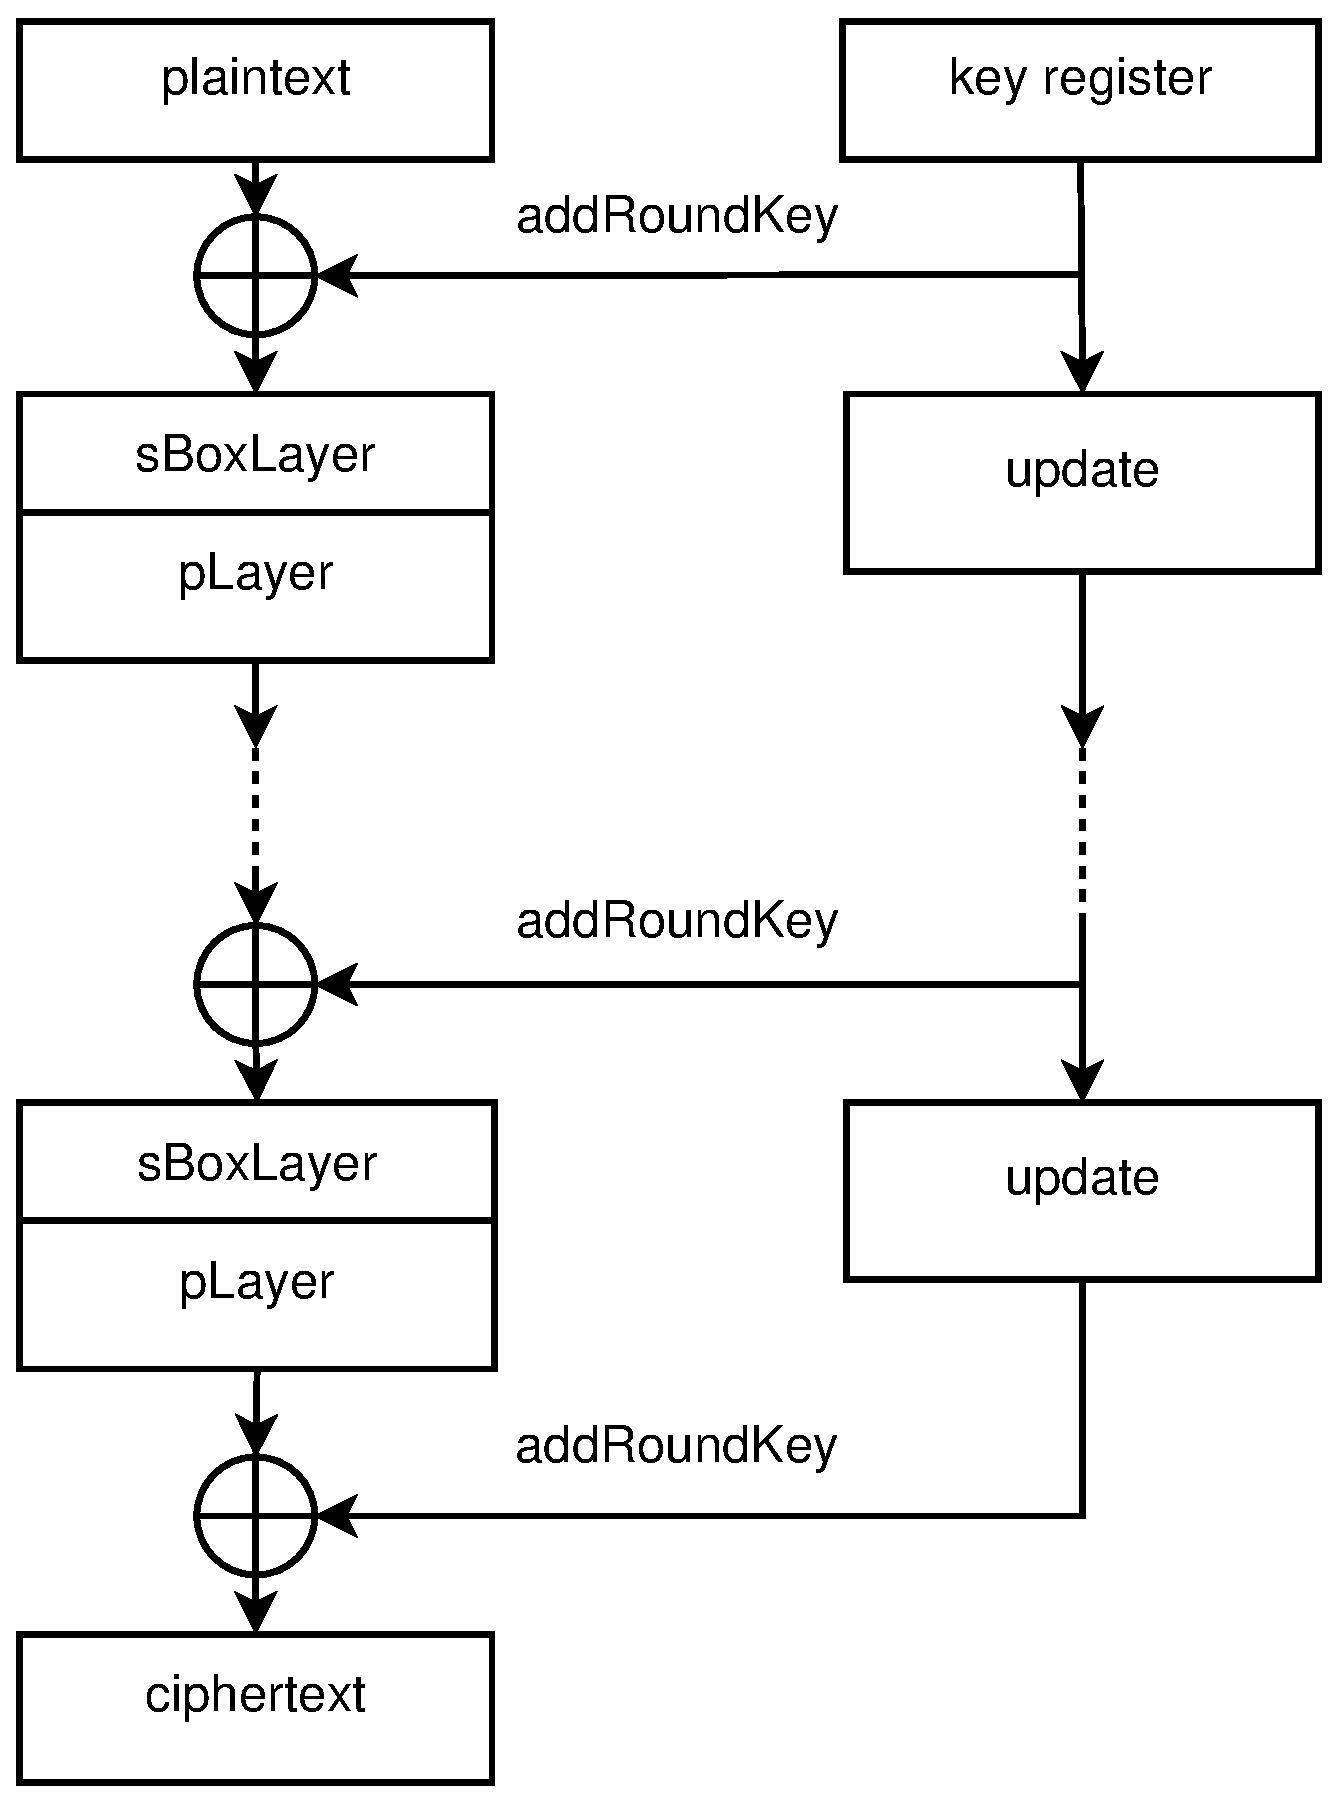
\includegraphics[scale=0.4]{cipher}
    \caption{PRESENT enciphering}
    \label{fig:present-cipher}
\end{figure}

\subsection{Substitution layer}

The nonlinear layer is represented by a single 4-bit substitution 
$ F_2^4 \rightarrow F_2^4 $. It is a direct outcome of strict constrains on
efficiency and implementation area. Some additional restrictions are applied on
S-box for reaching an avalanche effect. Let us denote the Fourier coefficient of
$ S $ by
\begin{equation}
    S_b^W(a) = \sum\limits_{x \in F_2^4} (-1)^{(b,  S(x)) + (a,  x)}.
\end{equation}

Than the PRESENT S-box (table~\ref{tbl:sbox}) meets the following
conditions:
\begin{enumerate}
    \setlength{\itemsep}{0pt}%
        \setlength{\parskip}{0pt}%
    \item for any fixed non-zero input difference  
        $ \Delta_I \in F_2^4 $ and any fixed non-zero output difference 
        $ \Delta_O \in F_2^4 $ it is required that
        \begin{equation}
            \# \left\{ x \in F_2^4 \, | \, S(x) + S(x + \Delta_I) = \Delta_O \right\}
            \leq 4;
        \end{equation}
    \item for any fixed non-zero input difference
        $ \Delta_I \in F_2^4 $ and any fixed output difference
        $ \Delta_O \in F_2^4 $ such that
        $ wt(\Delta_I) = wt(\Delta_O) = 1 $ the following is true
        \begin{equation}
            \# \left\{ x \in F_2^4 \, | \, S(x) + S(x + \Delta_I) = \Delta_O\ \right\} = 0;
        \end{equation}
    \item for all non-zero $ a \in F_2^4 $ and all non-zero $ b \in F_2^4 $
        it holds that $ \left| S_b^W (a) \right| \leq 8 $;
    \item for all $ a \in F_2^4 $ and all non-zero $ b \in F_2^4 $ such that
        $ wt(a) = wt(b) = 1 $ it holds that $ \left| S_b^W (a) \right| \leq 4 $.
\end{enumerate}
\begin{table}[p]
    \caption{PRESENT S-box}
    \label{tbl:sbox}
    \small
    \centering
    \begin{tabular}{|c||c|c|c|c|c|c|c|c|}
        \hline
        $ x $ & 0 & 1 & 2 & 3 & 4 & 5 & 6 & 7 \\ \hline
        $S[x]$& C & 5 & 6 & B & 9 & 0 & A & D \\ \hline
        $x$ & 8 & 9 & A & B & C & D & E & F \\ \hline
        $S[x] $ & 3 & E & F & 8 & 4 & 7 & 1 & 2 \\ \hline
    \end{tabular}
\end{table}
From entire set of S-boxes satisfying the specified conditions the one was chosen
with the most efficient hardware implementation (that is less logic gates
required for boolean representation). The boolean function of each S-box bit
after minimization is showed below: 

\noindent
$ S_0(x) = x_3 \cdot x_2 \cdot \overline{x_1} \cdot x_0 +
\overline{x_3} \cdot x_2 \cdot \overline{x_1} \cdot \overline{x_0} + 
\overline{x_3} \cdot \overline{x_2} \cdot \overline{x_1} \cdot x_0 +
x_3 \cdot x_1 \cdot \overline{x_0} + 
\overline{x_3} \cdot x_2 \cdot x_1 \cdot x_0 + 
\overline{x_3} \cdot \overline{x_2} \cdot x_1 \cdot x_0 +
x_3 \cdot \overline{x_2} \cdot \overline{x_0} $; 

\noindent
$ S_1(x) = \overline{x_3} \cdot x_2 \cdot x_1 \cdot \overline{x_0} + x_3 \cdot  
x_2 \cdot x_0 + \overline{x_2} \cdot {x_1} \cdot \overline{x_0} + x_3 \cdot 
\overline{x_2} \cdot \overline{x_1} \cdot x_0 + \overline{x_3} \cdot 
\overline{x_2} \cdot x_1 \cdot x_0 + x_3 \cdot \overline{x_2} \cdot
\overline{x_0} $;

\noindent
$ S_2(x) = \overline{x_3} \cdot \overline{x_2} \cdot \overline{x_1} \cdot
\overline{x_0} + \overline{x_3} \cdot \overline{x_2} \cdot \overline{x_1} \cdot 
x_0 + x_3 \cdot x_2 \cdot \overline{x_1} + \overline{x_3} \cdot x_2 \cdot x_1
\cdot x_0 + \overline{x_2} \cdot x_1 \cdot \overline{x_0} + x_3 \cdot
\overline{x_2} \cdot \overline{x_1} \cdot x_0 $;

\noindent
$ S_3(x) = \overline{x_3} \cdot x_2 \cdot x_1 \cdot \overline{x_0} +
\overline{x_3} \cdot \overline{x_2} \cdot \overline{x_1} \cdot \overline{x_0} +
\overline{x_3} \cdot x_2 \cdot \overline{x_1} \cdot \overline{x_0} + x_3 \cdot
\overline{x_2} \cdot x_1 + \overline{x_3} \cdot x_2 \cdot x_1 \cdot x_0 + x_3
\cdot \overline{x_2} \cdot \overline{x_1} \cdot x_0 + \overline{x_3} \cdot
\overline{x_2} \cdot x_1 \cdot x_0 $;

\noindent where $ \overline{x_i} $ denotes the inversion of $ x_i $ bit, 
$ \cdot $ denotes logical \verb+AND+, $ + $ denotes logical \verb+OR+.

\subsection{Permutation layer}

The main problem considered during the permutation layer
(table~\ref{tbl:player}) development was the number of required logic gates for
implementation. Functional representation of permutation is showed in formula
(\ref{eqn:player}).
\begin{equation}
    \label{eqn:player}
    P(i) = \left\{
    \begin{array}{ll}
        i \cdot 16 \mod 63, & i \in {0, \hdots, 62} \\
        63,  & i = 63.
    \end{array} \right.
\end{equation}

\begin{table}[p]
    \centering
    \caption{PRESENT permutation layer}
    \small
    \label{tbl:player}
    \begin{tabular}{|c||c|c|c|c|c|c|c|c|}
        \hline
        $ i $  & 0  & 1  & 2  & 3  & 4 & 5  & 6  & 7  \\[-0.8ex]
        $P(i)$ & 0  & 16 & 32 & 48 & 1 & 17 & 33 & 49 \\
        \hline
        $ i $  & 8 & 9  & 10 & 11 & 12 & 13 & 14 & 15 \\[-0.8ex] 
        $P(i)$ & 2 & 18 & 34 & 50 & 3  & 19 & 35 & 51 \\ 
        \hline

        $ i $  & 16 & 17 & 18 & 19 & 20 & 21 & 22 & 23 \\[-0.8ex]
        $P(i)$ & 4  & 20 & 36 & 52 & 5  & 21 & 37 & 53 \\
        \hline
        $ i $  & 24 & 25 & 26 & 27 & 28 & 29 & 30 & 31 \\[-0.8ex]
        $P(i)$ & 6  & 22 & 38 & 54 & 7  & 23 & 39 & 55 \\ 
        \hline

        $ i $  & 32 & 33 & 34 & 35 & 36 & 37 & 38 & 39 \\[-0.8ex] 
        $P(i)$ & 8  & 24 & 40 & 56 & 9  & 25 & 41 & 57 \\
        \hline
        $ i $  &  40 & 41 & 42 & 43 & 44 & 45 & 46 & 47 \\ [-0.8ex] 
        $P(i)$ &  10 & 26 & 42 & 58 & 11 & 27 & 43 & 59 \\ 
        \hline
        $ i $  & 48 & 49 & 50 & 51 & 52 & 53 & 54 & 55 \\[-0.8ex] 
        $P(i)$ & 12 & 28 & 44 & 60 & 13 & 29 & 45 & 61 \\
        \hline
        $ i $  & 56 & 57 & 58 & 59 & 60 & 61 & 62 & 63 \\ [-0.8ex] 
        $P(i)$ & 14 & 30 & 46 & 62 & 15 & 31 & 47 & 63 \\     
        \hline
    \end{tabular}
\end{table}

\subsection{The key schedule}

User key is stored in register $ K $ and is represented with a bit sequence
$ k_{79} k_{78} \hdots k_0 $. Each round the subkey consists of 64 most
significant (left) key register bits. After extracting another subkey the key
register state is updated as follows:
\begin{enumerate}
    \setlength{\itemsep}{1pt}
        \setlength{\parskip}{0pt}
        \setlength{\parsep}{0pt}
    \item $ [k_{79} k_{78} \hdots k_1 k_0] = [k_{18} k_{17} \hdots k_{20} k_{19}] $;
    \item $ [K_{79} k_{78} k_{77} k_{76}] = S[k_{79} k_{78} k_{77} k_{76}] $;
    \item $ [k_{19} k_{18} k_{17} k_{16} k_{15}] = [k_{19} k_{18} k_{17} k_{16}
        k_{15} \oplus \text{round\_counter}] $.
\end{enumerate}

\subsection{Deciphering}

Deciphering uses analogous inverse permutations. Subkeys are supplied in the
same order as during enciphering. The reverse S-box is showed in
table~\ref{tbl:invsbox}.
\begin{table}[hbp]
    \caption{Inverse S-box of PRESENT}
    \label{tbl:invsbox}
    \small
    \centering
    \begin{tabular}{|c||c|c|c|c|c|c|c|c|}
        \hline
        $ x $ & 0 & 1 & 2 & 3 & 4 & 5 & 6 & 7 \\
        \hline
        $S[x]$& 5 & E & F & 8 & C & 1 & 2 & D \\
        \hline
        $x$ & 8 & 9 & A & B & C & D & E & F \\
        \hline
        $S[x]$ & B & 4 & 6 & 3 & 0 & 7 & 9 & A \\ 
        \hline
    \end{tabular}
\end{table}
Inverse permutation layer is showed in table~\ref{tbl:invplayer}.
\begin{table}[p]
    \centering
    \caption{PRESENT inverse permutation layer}
    \label{tbl:invplayer}
    \small
    \begin{tabular}{|c||c|c|c|c|c|c|c|c|}
        \hline
        $ i $  & 0 & 1 & 2 & 3  & 4  & 5  & 6  & 7  \\[-0.8ex]
        $P(i)$ & 0 & 4 & 8 & 12 & 16 & 20 & 24 & 28 \\
        \hline
        $ i $  & 8  & 9  & 10 & 11 & 12 & 13 & 14 & 15 \\[-0.8ex]  
        $P(i)$ & 32 & 36 & 40 & 44 & 48 & 52 & 56 & 60 \\        
        \hline
        $ i $  & 16 & 17 & 18 & 19 & 20 & 21 & 22 & 23 \\[-0.8ex]
        $P(i)$ & 1  & 5  & 9  & 13 & 17 & 21 & 25 & 29 \\
        \hline
        $ i $  & 24 & 25 & 26 & 27 & 28 & 29 & 30 & 31 \\[-0.8ex] 
        $P(i)$ & 33 & 37 & 41 & 45 & 49 & 53 & 57 & 61 \\       
        \hline
        $ i $  & 32 & 33 & 34 & 35 & 36 & 37 & 38 & 39 \\[-0.8ex]
        $P(i)$ & 2  & 6  & 10 & 14 & 18 & 22 & 26 & 30 \\
        \hline
        $ i $  & 40 & 41 & 42 & 43 & 44 & 45 & 46 & 47 \\[-0.8ex] 
        $P(i)$ & 34 & 38 & 42 & 46 & 50 & 54 & 58 & 62 \\       
        \hline
        $ i $  & 48 & 49 & 50 & 51 & 52 & 53 & 54 & 55 \\[-0.8ex]
        $P(i)$ & 3  & 7  & 11 & 15 & 19 & 23 & 27 & 31 \\
        \hline
        $ i $  & 56 & 57 & 58 & 59 & 60 & 61 & 62 & 63 \\[-0.8ex] 
        $P(i)$ & 35 & 39 & 43 & 47 & 51 & 55 & 59 & 63 \\               
        \hline
    \end{tabular}
\end{table}

\section{PRESENT hardware implementation properties}

Cipher authors considered a wide variety of different target platforms ranging
from highly-optimized ASICs, over more flexible but still efficient low-cost
FPGAs to hardware-software co-design approaches and flexible software
implementations for 4-, 8-, 16- and 32-bit processors.

We will investigate the ASIC implementation as it is the most efficient one.

\subsection{Performance evaluation}

To assess the efficiency of implementation the developers used the following
metrics presented in table~\ref{tbl:lwc-dev-metrics}.

\begin{table}[htbp]
\centering
\caption{Development metrics for lightweight cipher}
\label{tbl:lwc-dev-metrics}
\begin{tabular}{|c|p{0.8\textwidth}|} \hline
    Area &
    Area requirements are usually measured in $ \mu m^2 $ , but this
    value depends on the fabrication technology and the standard cell
    library. In order to compare the area requirements independently it is
    common to state the area as gate equivalents [GE]. One GE is equivalent
    to the area which is required by the two-input NAND gate with the
    lowest driving strength of the appropriate technology. The area in GE is
    derived by dividing the area in $ \mu m^2 $ by the area of a two-input NAND
    gate.  \\ \hline
    Cycles & 
    Number of clock cycles to compute and read out the result. \\ \hline
    Time &
    The required amount of time for a certain operation can be
    calculated by dividing the amount of cycles by the operating 
    $ t = \frac{cycles}{freq} $. \\ \hline
    Throughput &
    The rate at which new output is produced with respect to
    time. The number of output bits is divided by the time, i.e. by the
    needed cycles and multiplied by the operating frequency. It is expressed
    in bits per second [bps]. \\ \hline
    Power &
    The power consumption is estimated on the gate level by
    Synopsys \verb+PowerCompiler+. It is provided in micro Watt $ [\mu W] $. \\ \hline
    Energy &
    The energy consumption denotes the power consumption over a
    certain time period.  It can be calculated by multiplying the power
    consumption with the required time of the operation. The energy
    consumption is provided in micro Joule $ [\mu J] $. \\ \hline
    Current &
    The power consumption divided by the typical core voltage. \\ \hline
    Efficiency &
    The area to throughput ratio is used as a measure of
    hardware efficiency. The hardware efficiency is calculated by dividing
    the area requirements by the throughput and is expressed in gate
    equivalents per bits per second $ \left[ \frac{GE}{bps} \right]$. \\ \hline
\end{tabular}
\end{table}

\subsection{Measurements}

Measurements of ASIC round-based PRESENT implementation on 180 nm manufacturing
technology with 4-bit datapath are done at 100 kHz frequency and presented below:

\begin{description}
    \setlength{\itemsep}{1pt}
        \setlength{\parskip}{0pt}
        \setlength{\parsep}{0pt}
    \item[throughput:] 11.7 Kbps;
    \item[area:] $ 1075 $ GE;
    \item[efficiency:] $ 10.89 $ $ \frac{bps}{GE} $;
    \item[current:] $ 2.78 $ $ \mu A $.
\end{description}

Serialized and parallelized architectures implementation is also possible and
described by authors in detail~\cite{secsi:2007}.

\subsection{Cryptographic security}

The substitution layer has been developed with the resistance to differential
and linear cryptanalysis in mind.
The maximum differential probability of a PRESENT S-box is $ 2^{-2} $ and so the
probability of a single 25-round differential characteristic is bounded by $
2^{-100} $.

Differential properties of the S-box are shown in
table~\ref{tbl:present-sbox-diff}.
\begin{table}[htbp]
    \centering
    \caption{PRESENT S-box differential properties}
    \label{tbl:present-sbox-diff}
    \begin{tabular}{|c|c|} \hline
        Differential & Number of occurrences \\ \hline
        0  &  159 \\ \hline
        2  &  72  \\ \hline
        4  &  24  \\ \hline
    \end{tabular}
\end{table}

Linear properties of the S-box are shown in table~\ref{tbl:present-sbox-lin}.
\begin{table}[htbp]
    \centering
    \caption{PRESENT S-box linear properties}
    \label{tbl:present-sbox-lin}
    \begin{tabular}{|c|c|} \hline
        Linear bias & Number of occurrences \\ \hline
        0 & 123 \\ \hline
        2 & 96  \\ \hline 
        4 & 36  \\ \hline 
    \end{tabular}
\end{table}

For approximating 28 cipher rounds with linear cryptanalysis one needs to obtain
$ 2^{84} $ \mbox{plaintext/ciphertext} pairs, which exceeds the set of all
possible plaintexts for PRESENT.

Integral attack on 7-round PRESENT requires $ 2^{43.3} $ chosen
plaintexts, has time complexity $ 2^{100.1} $ and requires $ 2^{77} $ bytes of
memory.

For applying an algebraic attack $ 11067 $ quadratic equations with $ 4216 $
variables have to be solved. Solving such equations is an NP-hard task.
Despite the successful attacks on small-scale versions of block ciphers the
increase of input block size results in enormous time and memory complexity.

The cipher security depends on key scheduling scheme. PRESENT uses round
counter XORing with key register to decrease the correlation between subkeys.
For the sake of nonlinearity while generating key material some bits pass
through S-box when the key register updates (table~\ref{tbl:sbox}). 

All bits in the key register are a nonlinear function of the 80-bit master key
by round 21. Each bit in the key register after round 21 depends on at least
four of the master key bits

By deriving $ K_{32} $, six bits are degree two expressions of the 80 master key
bits, 24 bits are of degree three, while the remaining bits are degree six or
degree nine function of the master key bits.

The statistical saturation attack can break 14 out of 31 rounds of
PRESENT and requires $ 2^{34} $ \mbox{plaintext/ciphertext}
pairs~\cite{collard:present}.

Side channel attacks as well as invasive attacks may be a threat for
PRESENT just like for any other cryptographic primitives.

\section{Comparison of PRESENT, GOST 28147-89 and AES}
\label{sec:lwc-comparison}

Advanced Encryption Standard (AES) is a symmetric block cipher, adopted
as the national encryption standard in USA. This algorithm is widely used in
the world and therefore very well researched.

GOST~28147-89 is a symmetric block cipher recommended for application in
Ukraine, it is also the encryption standard in Russia and other CIS countries,
adopted in 1989.The most efficient known attack breaks the cipher
only $ 2^8 $ times faster than a brute force. In 2010 the
GOST cipher was submitted to ISO to become also an international
standard. For a more detailed description of the cipher refer to
section~\ref{sec:algebraic-gost}.

In consideration of long-term analysis and wide usage of AES and
GOST~28147-89 the comparison of PRESENT with these ciphers is
necessary.

\subsection{Implementation complexity}

The PRESENT structure is incredibly simple. After some precomputations
the algorithm may be replaced with the lookup table and key addition. All cipher
operations can be successfully performed on 4-bit processor and do not require
complex calculations. The most compact implementation requires $ 1000 $ gate
equivalents.

AES has complex structure~\cite{daemen:rijndael}. It uses 8-bit S-box and
its storage requires significantly more memory than 4-bit S-box. For linear bit
diffusion the maximum distance separable (MDS) code based permutation is used.
MDS-permutation uses matrix multiplications in $ GF(2^8) $ and requires
substantial computer resources or additional precomputed lookup tables. Hardware
implementation fits on $ 3100 $ GE on 350 nm manufacturing process.

GOST~28147-89 represents a Feistel network. The cipher uses following
operations: modulo 32 addition, bitwise exclusive \verb+OR+, bitwise shift and a
substitution box. Software implementation for 32-bit processors overtops
PRESENT in throughput. The hardware implementation requires only $ 800 $
gate equivalents~\cite{poschmann:gost}.

\subsection{Cryptographic security}

AES has 128-bit input block size and possible key length of 128, 192 or
256 bits. Number of rounds depends on the key length (10, 12 or 14). Best known
attack on AES-256 has $ 2^{99.5} $ complexity but isn't applicable to
AES-128. Side channel attacks on some implementations might have less
complexity.

GOST~28147-89 has 64-bit input block size and the key length of 256 bits. 
Attack proposed by Nicolas Courtois requires $ 2^{64} $
\mbox{plaintext/ciphertext} pairs and speeds up cryptanalysis only by a factor
of $ 2^8 $ comparable to brute force~\cite{Courtois:cryptoeprint_2011}. It is worth noting,
however, that any cipher can be broken by generating a dictionary of
\mbox{plaintext/ciphertext} values for all possible inputs. Taking into account
the efficiency of PRESENT and its 64-bit input block size it is possible
to compute all \mbox{plaintext/ciphertext} pairs for foreseeable time using
appropriate computing powers.

In distinction from the described ciphers PRESENT has 80 bit key length.
The cipher is inapplicable for enciphering large data requiring high security level, but is
well suited for embedded devices and RFID tags where the moderate security level
for small data sequences is acceptable.

By comparison results GOST~28147-89 is also well suited for such
applications and betters PRESENT on some parameters.

\subsection{Efficiency}

Ciphers efficiency comparison is showed in table~\ref{tbl:comparison}. It is
worth noting that the examined PRESENT implementation described in~\cite{cryptoeprint:2009_516} is designed for
4-bit processor (handles 4 bits per tick) whereas AES and GOST are
unable to function on 4-bit processors. Data for GOST throughput values have
been extrapolated from the author's software implementation benchmarks and
normalized according to the described hardware characteristics
in~\cite{cryptoeprint:2009_516}, so the accuracy has some is not perfect.
\begin{table}[htbp]
    \centering
    \caption{Efficiency comparison of PRESENT, AES and GOST 28147}
    \label{tbl:comparison}
    \begin{tabular}{|l|p{1.5cm}|p{2cm}|p{2.8cm}|p{2.5cm}|p{2cm}|}
        \hline
        Cipher & Key & Block & Throughput, Kb/s & Area, GE & Eff., $\frac{bps}{GE}$ \\
        \hline
        GOST    & 256 & 64  & 14   & 800  & 17.5  \\
        \hline
        AES     & 128 & 128 & 80   & 3100 & 25.81 \\
        \hline
        PRESENT & 64  & 80  & 11.7 & 1075 & 10.89 \\
        \hline
    \end{tabular}
\end{table}

\section{Results of evaluation}

PRESENT cipher was specifically designed for hardware implementation
and functioning on ultra constrained devices. This fact explains design
decisions towards simple and high-speed permutations and 4-bit S-box applied to
the whole input block. The absence of computationally difficult operations
(multiplication, modulo addition) and lookup tables ensure compact
implementation, less area on a chip requirement and so --- cheap self-cost.

However the comparison for PRESENT, AES and GOST~28147-89
showed that GOST also fits for lightweight cryptography purposes and
a little bit better than PRESENT in implementation area. With slight
modification of the algorithm hardware implementation will require as little as
$ 651 $ GE. Unlike new PRESENT cipher GOST~28147-89 is well
time-tested and examined, also a wide variety of implementations already exists.

Taking into account the submitting of GOST cipher for international
enciphering standard, further research of the cipher applications on constrained
devices (energy consumption, side channel attacks resistance) is urgent. 

In turn, PRESENT can function on 4-bit processors and has more flexibility
for implementation that allows its effective use on devices with variate
architectures.


% Graphic for TeX using PGF
% Title: /home/zoresvit/Documents/research/diploma/graphics/zuc.dia
% Creator: Dia v0.97.1
% CreationDate: Fri Nov 11 01:43:40 2011
% For: zoresvit
% \usepackage{tikz}
% The following commands are not supported in PSTricks at present
% We define them conditionally, so when they are implemented,
% this pgf file will use them.
\ifx\du\undefined
  \newlength{\du}
\fi
\setlength{\du}{10\unitlength}

\begin{tikzpicture}[scale=0.55,every node/.style={scale=0.6}]

\pgftransformxscale{1.000000}
\pgftransformyscale{-1.000000}
\definecolor{dialinecolor}{rgb}{0.000000, 0.000000, 0.000000}
\pgfsetstrokecolor{dialinecolor}
\definecolor{dialinecolor}{rgb}{1.000000, 1.000000, 1.000000}
\pgfsetfillcolor{dialinecolor}
\pgfsetlinewidth{0.100000\du}
\pgfsetdash{{\pgflinewidth}{0.200000\du}}{0cm}
\pgfsetdash{{\pgflinewidth}{0.200000\du}}{0cm}
\pgfsetmiterjoin
\definecolor{dialinecolor}{rgb}{0.000000, 0.000000, 0.000000}
\pgfsetstrokecolor{dialinecolor}
\draw (7.000000\du,-3.000000\du)--(7.000000\du,7.000000\du)--(43.500000\du,7.000000\du)--(43.500000\du,-3.000000\du)--cycle;
% setfont left to latex
\definecolor{dialinecolor}{rgb}{0.000000, 0.000000, 0.000000}
\pgfsetstrokecolor{dialinecolor}
\node at (25.250000\du,2.195000\du){};
\pgfsetlinewidth{0.100000\du}
\pgfsetdash{{\pgflinewidth}{0.200000\du}}{0cm}
\pgfsetdash{{\pgflinewidth}{0.200000\du}}{0cm}
\pgfsetmiterjoin
\definecolor{dialinecolor}{rgb}{0.000000, 0.000000, 0.000000}
\pgfsetstrokecolor{dialinecolor}
\draw (7.000000\du,8.000000\du)--(7.000000\du,12.000000\du)--(43.500000\du,12.000000\du)--(43.500000\du,8.000000\du)--cycle;
% setfont left to latex
\definecolor{dialinecolor}{rgb}{0.000000, 0.000000, 0.000000}
\pgfsetstrokecolor{dialinecolor}
\node at (25.250000\du,10.195000\du){};
\pgfsetlinewidth{0.100000\du}
\pgfsetdash{{\pgflinewidth}{0.200000\du}}{0cm}
\pgfsetdash{{\pgflinewidth}{0.200000\du}}{0cm}
\pgfsetmiterjoin
\definecolor{dialinecolor}{rgb}{0.000000, 0.000000, 0.000000}
\pgfsetstrokecolor{dialinecolor}
\draw (7.100000\du,13.000000\du)--(7.100000\du,34.000000\du)--(32.100000\du,34.000000\du)--(32.100000\du,13.000000\du)--cycle;
% setfont left to latex
\definecolor{dialinecolor}{rgb}{0.000000, 0.000000, 0.000000}
\pgfsetstrokecolor{dialinecolor}
\node at (19.600000\du,23.695000\du){};
% setfont left to latex
\definecolor{dialinecolor}{rgb}{0.000000, 0.000000, 0.000000}
\pgfsetstrokecolor{dialinecolor}
\node[anchor=west] at (25.500000\du,1.500000\du){LFSR};
% setfont left to latex
\definecolor{dialinecolor}{rgb}{0.000000, 0.000000, 0.000000}
\pgfsetstrokecolor{dialinecolor}
\node[anchor=west] at (24.500000\du,9.000000\du){BR};
\definecolor{dialinecolor}{rgb}{1.000000, 1.000000, 1.000000}
\pgfsetfillcolor{dialinecolor}
\fill (40.000000\du,4.000000\du)--(40.000000\du,6.000000\du)--(42.000000\du,6.000000\du)--(42.000000\du,4.000000\du)--cycle;
\pgfsetlinewidth{0.100000\du}
\pgfsetdash{}{0pt}
\pgfsetdash{}{0pt}
\pgfsetmiterjoin
\definecolor{dialinecolor}{rgb}{0.000000, 0.000000, 0.000000}
\pgfsetstrokecolor{dialinecolor}
\draw (40.000000\du,4.000000\du)--(40.000000\du,6.000000\du)--(42.000000\du,6.000000\du)--(42.000000\du,4.000000\du)--cycle;
% setfont left to latex
\definecolor{dialinecolor}{rgb}{0.000000, 0.000000, 0.000000}
\pgfsetstrokecolor{dialinecolor}
\node at (41.000000\du,5.195000\du){$s_{0}$};
\definecolor{dialinecolor}{rgb}{1.000000, 1.000000, 1.000000}
\pgfsetfillcolor{dialinecolor}
\fill (38.000000\du,4.000000\du)--(38.000000\du,6.000000\du)--(40.000000\du,6.000000\du)--(40.000000\du,4.000000\du)--cycle;
\pgfsetlinewidth{0.100000\du}
\pgfsetdash{}{0pt}
\pgfsetdash{}{0pt}
\pgfsetmiterjoin
\definecolor{dialinecolor}{rgb}{0.000000, 0.000000, 0.000000}
\pgfsetstrokecolor{dialinecolor}
\draw (38.000000\du,4.000000\du)--(38.000000\du,6.000000\du)--(40.000000\du,6.000000\du)--(40.000000\du,4.000000\du)--cycle;
% setfont left to latex
\definecolor{dialinecolor}{rgb}{0.000000, 0.000000, 0.000000}
\pgfsetstrokecolor{dialinecolor}
\node at (39.000000\du,5.195000\du){$s_{1}$};
\definecolor{dialinecolor}{rgb}{1.000000, 1.000000, 1.000000}
\pgfsetfillcolor{dialinecolor}
\fill (36.000000\du,4.000000\du)--(36.000000\du,6.000000\du)--(38.000000\du,6.000000\du)--(38.000000\du,4.000000\du)--cycle;
\pgfsetlinewidth{0.100000\du}
\pgfsetdash{}{0pt}
\pgfsetdash{}{0pt}
\pgfsetmiterjoin
\definecolor{dialinecolor}{rgb}{0.000000, 0.000000, 0.000000}
\pgfsetstrokecolor{dialinecolor}
\draw (36.000000\du,4.000000\du)--(36.000000\du,6.000000\du)--(38.000000\du,6.000000\du)--(38.000000\du,4.000000\du)--cycle;
% setfont left to latex
\definecolor{dialinecolor}{rgb}{0.000000, 0.000000, 0.000000}
\pgfsetstrokecolor{dialinecolor}
\node at (37.000000\du,5.195000\du){$s_{2}$};
\definecolor{dialinecolor}{rgb}{1.000000, 1.000000, 1.000000}
\pgfsetfillcolor{dialinecolor}
\fill (34.000000\du,4.000000\du)--(34.000000\du,6.000000\du)--(36.000000\du,6.000000\du)--(36.000000\du,4.000000\du)--cycle;
\pgfsetlinewidth{0.100000\du}
\pgfsetdash{}{0pt}
\pgfsetdash{}{0pt}
\pgfsetmiterjoin
\definecolor{dialinecolor}{rgb}{0.000000, 0.000000, 0.000000}
\pgfsetstrokecolor{dialinecolor}
\draw (34.000000\du,4.000000\du)--(34.000000\du,6.000000\du)--(36.000000\du,6.000000\du)--(36.000000\du,4.000000\du)--cycle;
% setfont left to latex
\definecolor{dialinecolor}{rgb}{0.000000, 0.000000, 0.000000}
\pgfsetstrokecolor{dialinecolor}
\node at (35.000000\du,5.195000\du){$s_{3}$};
\definecolor{dialinecolor}{rgb}{1.000000, 1.000000, 1.000000}
\pgfsetfillcolor{dialinecolor}
\fill (32.000000\du,4.000000\du)--(32.000000\du,6.000000\du)--(34.000000\du,6.000000\du)--(34.000000\du,4.000000\du)--cycle;
\pgfsetlinewidth{0.100000\du}
\pgfsetdash{}{0pt}
\pgfsetdash{}{0pt}
\pgfsetmiterjoin
\definecolor{dialinecolor}{rgb}{0.000000, 0.000000, 0.000000}
\pgfsetstrokecolor{dialinecolor}
\draw (32.000000\du,4.000000\du)--(32.000000\du,6.000000\du)--(34.000000\du,6.000000\du)--(34.000000\du,4.000000\du)--cycle;
% setfont left to latex
\definecolor{dialinecolor}{rgb}{0.000000, 0.000000, 0.000000}
\pgfsetstrokecolor{dialinecolor}
\node at (33.000000\du,5.195000\du){$s_{4}$};
\definecolor{dialinecolor}{rgb}{1.000000, 1.000000, 1.000000}
\pgfsetfillcolor{dialinecolor}
\fill (30.000000\du,4.000000\du)--(30.000000\du,6.000000\du)--(32.000000\du,6.000000\du)--(32.000000\du,4.000000\du)--cycle;
\pgfsetlinewidth{0.100000\du}
\pgfsetdash{}{0pt}
\pgfsetdash{}{0pt}
\pgfsetmiterjoin
\definecolor{dialinecolor}{rgb}{0.000000, 0.000000, 0.000000}
\pgfsetstrokecolor{dialinecolor}
\draw (30.000000\du,4.000000\du)--(30.000000\du,6.000000\du)--(32.000000\du,6.000000\du)--(32.000000\du,4.000000\du)--cycle;
% setfont left to latex
\definecolor{dialinecolor}{rgb}{0.000000, 0.000000, 0.000000}
\pgfsetstrokecolor{dialinecolor}
\node at (31.000000\du,5.195000\du){$s_{5}$};
\definecolor{dialinecolor}{rgb}{1.000000, 1.000000, 1.000000}
\pgfsetfillcolor{dialinecolor}
\fill (28.000000\du,4.000000\du)--(28.000000\du,6.000000\du)--(30.000000\du,6.000000\du)--(30.000000\du,4.000000\du)--cycle;
\pgfsetlinewidth{0.100000\du}
\pgfsetdash{}{0pt}
\pgfsetdash{}{0pt}
\pgfsetmiterjoin
\definecolor{dialinecolor}{rgb}{0.000000, 0.000000, 0.000000}
\pgfsetstrokecolor{dialinecolor}
\draw (28.000000\du,4.000000\du)--(28.000000\du,6.000000\du)--(30.000000\du,6.000000\du)--(30.000000\du,4.000000\du)--cycle;
% setfont left to latex
\definecolor{dialinecolor}{rgb}{0.000000, 0.000000, 0.000000}
\pgfsetstrokecolor{dialinecolor}
\node at (29.000000\du,5.195000\du){$s_{6}$};
\definecolor{dialinecolor}{rgb}{1.000000, 1.000000, 1.000000}
\pgfsetfillcolor{dialinecolor}
\fill (26.000000\du,4.000000\du)--(26.000000\du,6.000000\du)--(28.000000\du,6.000000\du)--(28.000000\du,4.000000\du)--cycle;
\pgfsetlinewidth{0.100000\du}
\pgfsetdash{}{0pt}
\pgfsetdash{}{0pt}
\pgfsetmiterjoin
\definecolor{dialinecolor}{rgb}{0.000000, 0.000000, 0.000000}
\pgfsetstrokecolor{dialinecolor}
\draw (26.000000\du,4.000000\du)--(26.000000\du,6.000000\du)--(28.000000\du,6.000000\du)--(28.000000\du,4.000000\du)--cycle;
% setfont left to latex
\definecolor{dialinecolor}{rgb}{0.000000, 0.000000, 0.000000}
\pgfsetstrokecolor{dialinecolor}
\node at (27.000000\du,5.195000\du){$s_{7}$};
\definecolor{dialinecolor}{rgb}{1.000000, 1.000000, 1.000000}
\pgfsetfillcolor{dialinecolor}
\fill (24.000000\du,4.000000\du)--(24.000000\du,6.000000\du)--(26.000000\du,6.000000\du)--(26.000000\du,4.000000\du)--cycle;
\pgfsetlinewidth{0.100000\du}
\pgfsetdash{}{0pt}
\pgfsetdash{}{0pt}
\pgfsetmiterjoin
\definecolor{dialinecolor}{rgb}{0.000000, 0.000000, 0.000000}
\pgfsetstrokecolor{dialinecolor}
\draw (24.000000\du,4.000000\du)--(24.000000\du,6.000000\du)--(26.000000\du,6.000000\du)--(26.000000\du,4.000000\du)--cycle;
% setfont left to latex
\definecolor{dialinecolor}{rgb}{0.000000, 0.000000, 0.000000}
\pgfsetstrokecolor{dialinecolor}
\node at (25.000000\du,5.195000\du){$s_{8}$};
\definecolor{dialinecolor}{rgb}{1.000000, 1.000000, 1.000000}
\pgfsetfillcolor{dialinecolor}
\fill (22.000000\du,4.000000\du)--(22.000000\du,6.000000\du)--(24.000000\du,6.000000\du)--(24.000000\du,4.000000\du)--cycle;
\pgfsetlinewidth{0.100000\du}
\pgfsetdash{}{0pt}
\pgfsetdash{}{0pt}
\pgfsetmiterjoin
\definecolor{dialinecolor}{rgb}{0.000000, 0.000000, 0.000000}
\pgfsetstrokecolor{dialinecolor}
\draw (22.000000\du,4.000000\du)--(22.000000\du,6.000000\du)--(24.000000\du,6.000000\du)--(24.000000\du,4.000000\du)--cycle;
% setfont left to latex
\definecolor{dialinecolor}{rgb}{0.000000, 0.000000, 0.000000}
\pgfsetstrokecolor{dialinecolor}
\node at (23.000000\du,5.195000\du){$s_{9}$};
\definecolor{dialinecolor}{rgb}{1.000000, 1.000000, 1.000000}
\pgfsetfillcolor{dialinecolor}
\fill (19.800000\du,4.000000\du)--(19.800000\du,6.000000\du)--(22.050000\du,6.000000\du)--(22.050000\du,4.000000\du)--cycle;
\pgfsetlinewidth{0.100000\du}
\pgfsetdash{}{0pt}
\pgfsetdash{}{0pt}
\pgfsetmiterjoin
\definecolor{dialinecolor}{rgb}{0.000000, 0.000000, 0.000000}
\pgfsetstrokecolor{dialinecolor}
\draw (19.800000\du,4.000000\du)--(19.800000\du,6.000000\du)--(22.050000\du,6.000000\du)--(22.050000\du,4.000000\du)--cycle;
% setfont left to latex
\definecolor{dialinecolor}{rgb}{0.000000, 0.000000, 0.000000}
\pgfsetstrokecolor{dialinecolor}
\node at (20.925000\du,5.195000\du){$s_{10}$};
\definecolor{dialinecolor}{rgb}{1.000000, 1.000000, 1.000000}
\pgfsetfillcolor{dialinecolor}
\fill (17.800000\du,4.000000\du)--(17.800000\du,6.000000\du)--(20.050000\du,6.000000\du)--(20.050000\du,4.000000\du)--cycle;
\pgfsetlinewidth{0.100000\du}
\pgfsetdash{}{0pt}
\pgfsetdash{}{0pt}
\pgfsetmiterjoin
\definecolor{dialinecolor}{rgb}{0.000000, 0.000000, 0.000000}
\pgfsetstrokecolor{dialinecolor}
\draw (17.800000\du,4.000000\du)--(17.800000\du,6.000000\du)--(20.050000\du,6.000000\du)--(20.050000\du,4.000000\du)--cycle;
% setfont left to latex
\definecolor{dialinecolor}{rgb}{0.000000, 0.000000, 0.000000}
\pgfsetstrokecolor{dialinecolor}
\node at (18.925000\du,5.195000\du){$s_{11}$};
\definecolor{dialinecolor}{rgb}{1.000000, 1.000000, 1.000000}
\pgfsetfillcolor{dialinecolor}
\fill (15.600000\du,4.000000\du)--(15.600000\du,6.000000\du)--(17.850000\du,6.000000\du)--(17.850000\du,4.000000\du)--cycle;
\pgfsetlinewidth{0.100000\du}
\pgfsetdash{}{0pt}
\pgfsetdash{}{0pt}
\pgfsetmiterjoin
\definecolor{dialinecolor}{rgb}{0.000000, 0.000000, 0.000000}
\pgfsetstrokecolor{dialinecolor}
\draw (15.600000\du,4.000000\du)--(15.600000\du,6.000000\du)--(17.850000\du,6.000000\du)--(17.850000\du,4.000000\du)--cycle;
% setfont left to latex
\definecolor{dialinecolor}{rgb}{0.000000, 0.000000, 0.000000}
\pgfsetstrokecolor{dialinecolor}
\node at (16.725000\du,5.195000\du){$s_{12}$};
\definecolor{dialinecolor}{rgb}{1.000000, 1.000000, 1.000000}
\pgfsetfillcolor{dialinecolor}
\fill (13.475000\du,4.000000\du)--(13.475000\du,6.000000\du)--(15.725000\du,6.000000\du)--(15.725000\du,4.000000\du)--cycle;
\pgfsetlinewidth{0.100000\du}
\pgfsetdash{}{0pt}
\pgfsetdash{}{0pt}
\pgfsetmiterjoin
\definecolor{dialinecolor}{rgb}{0.000000, 0.000000, 0.000000}
\pgfsetstrokecolor{dialinecolor}
\draw (13.475000\du,4.000000\du)--(13.475000\du,6.000000\du)--(15.725000\du,6.000000\du)--(15.725000\du,4.000000\du)--cycle;
% setfont left to latex
\definecolor{dialinecolor}{rgb}{0.000000, 0.000000, 0.000000}
\pgfsetstrokecolor{dialinecolor}
\node at (14.600000\du,5.195000\du){$s_{13}$};
\definecolor{dialinecolor}{rgb}{1.000000, 1.000000, 1.000000}
\pgfsetfillcolor{dialinecolor}
\fill (11.275000\du,4.000000\du)--(11.275000\du,6.000000\du)--(13.525000\du,6.000000\du)--(13.525000\du,4.000000\du)--cycle;
\pgfsetlinewidth{0.100000\du}
\pgfsetdash{}{0pt}
\pgfsetdash{}{0pt}
\pgfsetmiterjoin
\definecolor{dialinecolor}{rgb}{0.000000, 0.000000, 0.000000}
\pgfsetstrokecolor{dialinecolor}
\draw (11.275000\du,4.000000\du)--(11.275000\du,6.000000\du)--(13.525000\du,6.000000\du)--(13.525000\du,4.000000\du)--cycle;
% setfont left to latex
\definecolor{dialinecolor}{rgb}{0.000000, 0.000000, 0.000000}
\pgfsetstrokecolor{dialinecolor}
\node at (12.400000\du,5.195000\du){$s_{14}$};
\definecolor{dialinecolor}{rgb}{1.000000, 1.000000, 1.000000}
\pgfsetfillcolor{dialinecolor}
\fill (9.000000\du,4.000000\du)--(9.000000\du,6.000000\du)--(11.250000\du,6.000000\du)--(11.250000\du,4.000000\du)--cycle;
\pgfsetlinewidth{0.100000\du}
\pgfsetdash{}{0pt}
\pgfsetdash{}{0pt}
\pgfsetmiterjoin
\definecolor{dialinecolor}{rgb}{0.000000, 0.000000, 0.000000}
\pgfsetstrokecolor{dialinecolor}
\draw (9.000000\du,4.000000\du)--(9.000000\du,6.000000\du)--(11.250000\du,6.000000\du)--(11.250000\du,4.000000\du)--cycle;
% setfont left to latex
\definecolor{dialinecolor}{rgb}{0.000000, 0.000000, 0.000000}
\pgfsetstrokecolor{dialinecolor}
\node at (10.125000\du,5.195000\du){$s_{15}$};
\definecolor{dialinecolor}{rgb}{1.000000, 1.000000, 1.000000}
\pgfsetfillcolor{dialinecolor}
\fill (9.000000\du,-2.000000\du)--(9.000000\du,0.000000\du)--(42.000000\du,0.000000\du)--(42.000000\du,-2.000000\du)--cycle;
\pgfsetlinewidth{0.100000\du}
\pgfsetdash{}{0pt}
\pgfsetdash{}{0pt}
\pgfsetmiterjoin
\definecolor{dialinecolor}{rgb}{0.000000, 0.000000, 0.000000}
\pgfsetstrokecolor{dialinecolor}
\draw (9.000000\du,-2.000000\du)--(9.000000\du,0.000000\du)--(42.000000\du,0.000000\du)--(42.000000\du,-2.000000\du)--cycle;
% setfont left to latex
\definecolor{dialinecolor}{rgb}{0.000000, 0.000000, 0.000000}
\pgfsetstrokecolor{dialinecolor}
\node at (25.500000\du,-0.805000\du){$\mod 2^{31} - 1$};
\pgfsetlinewidth{0.100000\du}
\pgfsetdash{}{0pt}
\pgfsetdash{}{0pt}
\pgfsetbuttcap
\pgfsetmiterjoin
\pgfsetlinewidth{0.100000\du}
\pgfsetbuttcap
\pgfsetmiterjoin
\pgfsetdash{}{0pt}
\definecolor{dialinecolor}{rgb}{1.000000, 1.000000, 1.000000}
\pgfsetfillcolor{dialinecolor}
\pgfpathmoveto{\pgfpoint{39.655000\du}{1.200000\du}}
\pgfpathlineto{\pgfpoint{41.475000\du}{1.200000\du}}
\pgfpathcurveto{\pgfpoint{41.726290\du}{1.200000\du}}{\pgfpoint{41.930000\du}{1.513401\du}}{\pgfpoint{41.930000\du}{1.900000\du}}
\pgfpathcurveto{\pgfpoint{41.930000\du}{2.286600\du}}{\pgfpoint{41.726290\du}{2.600000\du}}{\pgfpoint{41.475000\du}{2.600000\du}}
\pgfpathlineto{\pgfpoint{39.655000\du}{2.600000\du}}
\pgfpathcurveto{\pgfpoint{39.403710\du}{2.600000\du}}{\pgfpoint{39.200000\du}{2.286600\du}}{\pgfpoint{39.200000\du}{1.900000\du}}
\pgfpathcurveto{\pgfpoint{39.200000\du}{1.513401\du}}{\pgfpoint{39.403710\du}{1.200000\du}}{\pgfpoint{39.655000\du}{1.200000\du}}
\pgfusepath{fill}
\definecolor{dialinecolor}{rgb}{0.000000, 0.000000, 0.000000}
\pgfsetstrokecolor{dialinecolor}
\pgfpathmoveto{\pgfpoint{39.655000\du}{1.200000\du}}
\pgfpathlineto{\pgfpoint{41.475000\du}{1.200000\du}}
\pgfpathcurveto{\pgfpoint{41.726290\du}{1.200000\du}}{\pgfpoint{41.930000\du}{1.513401\du}}{\pgfpoint{41.930000\du}{1.900000\du}}
\pgfpathcurveto{\pgfpoint{41.930000\du}{2.286600\du}}{\pgfpoint{41.726290\du}{2.600000\du}}{\pgfpoint{41.475000\du}{2.600000\du}}
\pgfpathlineto{\pgfpoint{39.655000\du}{2.600000\du}}
\pgfpathcurveto{\pgfpoint{39.403710\du}{2.600000\du}}{\pgfpoint{39.200000\du}{2.286600\du}}{\pgfpoint{39.200000\du}{1.900000\du}}
\pgfpathcurveto{\pgfpoint{39.200000\du}{1.513401\du}}{\pgfpoint{39.403710\du}{1.200000\du}}{\pgfpoint{39.655000\du}{1.200000\du}}
\pgfusepath{stroke}
% setfont left to latex
\definecolor{dialinecolor}{rgb}{0.000000, 0.000000, 0.000000}
\pgfsetstrokecolor{dialinecolor}
\node at (40.565000\du,2.032292\du){$\scriptstyle 2^8 + 1$};
\pgfsetlinewidth{0.100000\du}
\pgfsetdash{}{0pt}
\pgfsetdash{}{0pt}
\pgfsetbuttcap
{
\definecolor{dialinecolor}{rgb}{0.000000, 0.000000, 0.000000}
\pgfsetfillcolor{dialinecolor}
% was here!!!
\pgfsetarrowsend{latex}
\definecolor{dialinecolor}{rgb}{0.000000, 0.000000, 0.000000}
\pgfsetstrokecolor{dialinecolor}
\draw (41.000000\du,3.949707\du)--(41.000000\du,2.600000\du);
}
\pgfsetlinewidth{0.100000\du}
\pgfsetdash{}{0pt}
\pgfsetdash{}{0pt}
\pgfsetbuttcap
{
\definecolor{dialinecolor}{rgb}{0.000000, 0.000000, 0.000000}
\pgfsetfillcolor{dialinecolor}
% was here!!!
\pgfsetarrowsend{latex}
\definecolor{dialinecolor}{rgb}{0.000000, 0.000000, 0.000000}
\pgfsetstrokecolor{dialinecolor}
\draw (41.020000\du,1.200000\du)--(41.000000\du,0.000000\du);
}
\pgfsetlinewidth{0.100000\du}
\pgfsetdash{}{0pt}
\pgfsetdash{}{0pt}
\pgfsetbuttcap
\pgfsetmiterjoin
\pgfsetlinewidth{0.100000\du}
\pgfsetbuttcap
\pgfsetmiterjoin
\pgfsetdash{}{0pt}
\definecolor{dialinecolor}{rgb}{1.000000, 1.000000, 1.000000}
\pgfsetfillcolor{dialinecolor}
\pgfpathmoveto{\pgfpoint{32.366250\du}{1.200000\du}}
\pgfpathlineto{\pgfpoint{33.831250\du}{1.200000\du}}
\pgfpathcurveto{\pgfpoint{34.033524\du}{1.200000\du}}{\pgfpoint{34.197500\du}{1.513401\du}}{\pgfpoint{34.197500\du}{1.900000\du}}
\pgfpathcurveto{\pgfpoint{34.197500\du}{2.286600\du}}{\pgfpoint{34.033524\du}{2.600000\du}}{\pgfpoint{33.831250\du}{2.600000\du}}
\pgfpathlineto{\pgfpoint{32.366250\du}{2.600000\du}}
\pgfpathcurveto{\pgfpoint{32.163976\du}{2.600000\du}}{\pgfpoint{32.000000\du}{2.286600\du}}{\pgfpoint{32.000000\du}{1.900000\du}}
\pgfpathcurveto{\pgfpoint{32.000000\du}{1.513401\du}}{\pgfpoint{32.163976\du}{1.200000\du}}{\pgfpoint{32.366250\du}{1.200000\du}}
\pgfusepath{fill}
\definecolor{dialinecolor}{rgb}{0.000000, 0.000000, 0.000000}
\pgfsetstrokecolor{dialinecolor}
\pgfpathmoveto{\pgfpoint{32.366250\du}{1.200000\du}}
\pgfpathlineto{\pgfpoint{33.831250\du}{1.200000\du}}
\pgfpathcurveto{\pgfpoint{34.033524\du}{1.200000\du}}{\pgfpoint{34.197500\du}{1.513401\du}}{\pgfpoint{34.197500\du}{1.900000\du}}
\pgfpathcurveto{\pgfpoint{34.197500\du}{2.286600\du}}{\pgfpoint{34.033524\du}{2.600000\du}}{\pgfpoint{33.831250\du}{2.600000\du}}
\pgfpathlineto{\pgfpoint{32.366250\du}{2.600000\du}}
\pgfpathcurveto{\pgfpoint{32.163976\du}{2.600000\du}}{\pgfpoint{32.000000\du}{2.286600\du}}{\pgfpoint{32.000000\du}{1.900000\du}}
\pgfpathcurveto{\pgfpoint{32.000000\du}{1.513401\du}}{\pgfpoint{32.163976\du}{1.200000\du}}{\pgfpoint{32.366250\du}{1.200000\du}}
\pgfusepath{stroke}
% setfont left to latex
\definecolor{dialinecolor}{rgb}{0.000000, 0.000000, 0.000000}
\pgfsetstrokecolor{dialinecolor}
\node at (33.098750\du,2.032292\du){$2^{20}$};
\pgfsetlinewidth{0.100000\du}
\pgfsetdash{}{0pt}
\pgfsetdash{}{0pt}
\pgfsetbuttcap
{
\definecolor{dialinecolor}{rgb}{0.000000, 0.000000, 0.000000}
\pgfsetfillcolor{dialinecolor}
% was here!!!
\pgfsetarrowsend{latex}
\definecolor{dialinecolor}{rgb}{0.000000, 0.000000, 0.000000}
\pgfsetstrokecolor{dialinecolor}
\draw (33.000000\du,4.000000\du)--(33.000000\du,2.600000\du);
}
\pgfsetlinewidth{0.100000\du}
\pgfsetdash{}{0pt}
\pgfsetdash{}{0pt}
\pgfsetbuttcap
{
\definecolor{dialinecolor}{rgb}{0.000000, 0.000000, 0.000000}
\pgfsetfillcolor{dialinecolor}
% was here!!!
\pgfsetarrowsend{latex}
\definecolor{dialinecolor}{rgb}{0.000000, 0.000000, 0.000000}
\pgfsetstrokecolor{dialinecolor}
\draw (33.000000\du,1.200000\du)--(33.000000\du,0.000000\du);
}
\pgfsetlinewidth{0.100000\du}
\pgfsetdash{}{0pt}
\pgfsetdash{}{0pt}
\pgfsetbuttcap
\pgfsetmiterjoin
\pgfsetlinewidth{0.100000\du}
\pgfsetbuttcap
\pgfsetmiterjoin
\pgfsetdash{}{0pt}
\definecolor{dialinecolor}{rgb}{1.000000, 1.000000, 1.000000}
\pgfsetfillcolor{dialinecolor}
\pgfpathmoveto{\pgfpoint{20.366250\du}{1.200000\du}}
\pgfpathlineto{\pgfpoint{21.831250\du}{1.200000\du}}
\pgfpathcurveto{\pgfpoint{22.033524\du}{1.200000\du}}{\pgfpoint{22.197500\du}{1.513401\du}}{\pgfpoint{22.197500\du}{1.900000\du}}
\pgfpathcurveto{\pgfpoint{22.197500\du}{2.286600\du}}{\pgfpoint{22.033524\du}{2.600000\du}}{\pgfpoint{21.831250\du}{2.600000\du}}
\pgfpathlineto{\pgfpoint{20.366250\du}{2.600000\du}}
\pgfpathcurveto{\pgfpoint{20.163976\du}{2.600000\du}}{\pgfpoint{20.000000\du}{2.286600\du}}{\pgfpoint{20.000000\du}{1.900000\du}}
\pgfpathcurveto{\pgfpoint{20.000000\du}{1.513401\du}}{\pgfpoint{20.163976\du}{1.200000\du}}{\pgfpoint{20.366250\du}{1.200000\du}}
\pgfusepath{fill}
\definecolor{dialinecolor}{rgb}{0.000000, 0.000000, 0.000000}
\pgfsetstrokecolor{dialinecolor}
\pgfpathmoveto{\pgfpoint{20.366250\du}{1.200000\du}}
\pgfpathlineto{\pgfpoint{21.831250\du}{1.200000\du}}
\pgfpathcurveto{\pgfpoint{22.033524\du}{1.200000\du}}{\pgfpoint{22.197500\du}{1.513401\du}}{\pgfpoint{22.197500\du}{1.900000\du}}
\pgfpathcurveto{\pgfpoint{22.197500\du}{2.286600\du}}{\pgfpoint{22.033524\du}{2.600000\du}}{\pgfpoint{21.831250\du}{2.600000\du}}
\pgfpathlineto{\pgfpoint{20.366250\du}{2.600000\du}}
\pgfpathcurveto{\pgfpoint{20.163976\du}{2.600000\du}}{\pgfpoint{20.000000\du}{2.286600\du}}{\pgfpoint{20.000000\du}{1.900000\du}}
\pgfpathcurveto{\pgfpoint{20.000000\du}{1.513401\du}}{\pgfpoint{20.163976\du}{1.200000\du}}{\pgfpoint{20.366250\du}{1.200000\du}}
\pgfusepath{stroke}
% setfont left to latex
\definecolor{dialinecolor}{rgb}{0.000000, 0.000000, 0.000000}
\pgfsetstrokecolor{dialinecolor}
\node at (21.098750\du,2.032292\du){$2^{21}$};
\pgfsetlinewidth{0.100000\du}
\pgfsetdash{}{0pt}
\pgfsetdash{}{0pt}
\pgfsetbuttcap
{
\definecolor{dialinecolor}{rgb}{0.000000, 0.000000, 0.000000}
\pgfsetfillcolor{dialinecolor}
% was here!!!
\pgfsetarrowsend{latex}
\definecolor{dialinecolor}{rgb}{0.000000, 0.000000, 0.000000}
\pgfsetstrokecolor{dialinecolor}
\draw (21.200000\du,4.000000\du)--(21.200000\du,2.600000\du);
}
\pgfsetlinewidth{0.100000\du}
\pgfsetdash{}{0pt}
\pgfsetdash{}{0pt}
\pgfsetbuttcap
{
\definecolor{dialinecolor}{rgb}{0.000000, 0.000000, 0.000000}
\pgfsetfillcolor{dialinecolor}
% was here!!!
\pgfsetarrowsend{latex}
\definecolor{dialinecolor}{rgb}{0.000000, 0.000000, 0.000000}
\pgfsetstrokecolor{dialinecolor}
\draw (21.200000\du,1.200000\du)--(21.200000\du,0.000000\du);
}
\pgfsetlinewidth{0.100000\du}
\pgfsetdash{}{0pt}
\pgfsetdash{}{0pt}
\pgfsetbuttcap
\pgfsetmiterjoin
\pgfsetlinewidth{0.100000\du}
\pgfsetbuttcap
\pgfsetmiterjoin
\pgfsetdash{}{0pt}
\definecolor{dialinecolor}{rgb}{1.000000, 1.000000, 1.000000}
\pgfsetfillcolor{dialinecolor}
\pgfpathmoveto{\pgfpoint{13.966250\du}{1.200000\du}}
\pgfpathlineto{\pgfpoint{15.431250\du}{1.200000\du}}
\pgfpathcurveto{\pgfpoint{15.633524\du}{1.200000\du}}{\pgfpoint{15.797500\du}{1.513401\du}}{\pgfpoint{15.797500\du}{1.900000\du}}
\pgfpathcurveto{\pgfpoint{15.797500\du}{2.286600\du}}{\pgfpoint{15.633524\du}{2.600000\du}}{\pgfpoint{15.431250\du}{2.600000\du}}
\pgfpathlineto{\pgfpoint{13.966250\du}{2.600000\du}}
\pgfpathcurveto{\pgfpoint{13.763976\du}{2.600000\du}}{\pgfpoint{13.600000\du}{2.286600\du}}{\pgfpoint{13.600000\du}{1.900000\du}}
\pgfpathcurveto{\pgfpoint{13.600000\du}{1.513401\du}}{\pgfpoint{13.763976\du}{1.200000\du}}{\pgfpoint{13.966250\du}{1.200000\du}}
\pgfusepath{fill}
\definecolor{dialinecolor}{rgb}{0.000000, 0.000000, 0.000000}
\pgfsetstrokecolor{dialinecolor}
\pgfpathmoveto{\pgfpoint{13.966250\du}{1.200000\du}}
\pgfpathlineto{\pgfpoint{15.431250\du}{1.200000\du}}
\pgfpathcurveto{\pgfpoint{15.633524\du}{1.200000\du}}{\pgfpoint{15.797500\du}{1.513401\du}}{\pgfpoint{15.797500\du}{1.900000\du}}
\pgfpathcurveto{\pgfpoint{15.797500\du}{2.286600\du}}{\pgfpoint{15.633524\du}{2.600000\du}}{\pgfpoint{15.431250\du}{2.600000\du}}
\pgfpathlineto{\pgfpoint{13.966250\du}{2.600000\du}}
\pgfpathcurveto{\pgfpoint{13.763976\du}{2.600000\du}}{\pgfpoint{13.600000\du}{2.286600\du}}{\pgfpoint{13.600000\du}{1.900000\du}}
\pgfpathcurveto{\pgfpoint{13.600000\du}{1.513401\du}}{\pgfpoint{13.763976\du}{1.200000\du}}{\pgfpoint{13.966250\du}{1.200000\du}}
\pgfusepath{stroke}
% setfont left to latex
\definecolor{dialinecolor}{rgb}{0.000000, 0.000000, 0.000000}
\pgfsetstrokecolor{dialinecolor}
\node at (14.698750\du,2.032292\du){$2^{15}$};
\pgfsetlinewidth{0.100000\du}
\pgfsetdash{}{0pt}
\pgfsetdash{}{0pt}
\pgfsetbuttcap
{
\definecolor{dialinecolor}{rgb}{0.000000, 0.000000, 0.000000}
\pgfsetfillcolor{dialinecolor}
% was here!!!
\pgfsetarrowsend{latex}
\definecolor{dialinecolor}{rgb}{0.000000, 0.000000, 0.000000}
\pgfsetstrokecolor{dialinecolor}
\draw (14.600000\du,4.000000\du)--(14.600000\du,2.600000\du);
}
\pgfsetlinewidth{0.100000\du}
\pgfsetdash{}{0pt}
\pgfsetdash{}{0pt}
\pgfsetbuttcap
{
\definecolor{dialinecolor}{rgb}{0.000000, 0.000000, 0.000000}
\pgfsetfillcolor{dialinecolor}
% was here!!!
\pgfsetarrowsend{latex}
\definecolor{dialinecolor}{rgb}{0.000000, 0.000000, 0.000000}
\pgfsetstrokecolor{dialinecolor}
\draw (14.600000\du,1.200000\du)--(14.600000\du,0.000000\du);
}
\pgfsetlinewidth{0.100000\du}
\pgfsetdash{}{0pt}
\pgfsetdash{}{0pt}
\pgfsetbuttcap
\pgfsetmiterjoin
\pgfsetlinewidth{0.100000\du}
\pgfsetbuttcap
\pgfsetmiterjoin
\pgfsetdash{}{0pt}
\definecolor{dialinecolor}{rgb}{1.000000, 1.000000, 1.000000}
\pgfsetfillcolor{dialinecolor}
\pgfpathmoveto{\pgfpoint{9.366250\du}{1.200000\du}}
\pgfpathlineto{\pgfpoint{10.831250\du}{1.200000\du}}
\pgfpathcurveto{\pgfpoint{11.033524\du}{1.200000\du}}{\pgfpoint{11.197500\du}{1.513401\du}}{\pgfpoint{11.197500\du}{1.900000\du}}
\pgfpathcurveto{\pgfpoint{11.197500\du}{2.286600\du}}{\pgfpoint{11.033524\du}{2.600000\du}}{\pgfpoint{10.831250\du}{2.600000\du}}
\pgfpathlineto{\pgfpoint{9.366250\du}{2.600000\du}}
\pgfpathcurveto{\pgfpoint{9.163976\du}{2.600000\du}}{\pgfpoint{9.000000\du}{2.286600\du}}{\pgfpoint{9.000000\du}{1.900000\du}}
\pgfpathcurveto{\pgfpoint{9.000000\du}{1.513401\du}}{\pgfpoint{9.163976\du}{1.200000\du}}{\pgfpoint{9.366250\du}{1.200000\du}}
\pgfusepath{fill}
\definecolor{dialinecolor}{rgb}{0.000000, 0.000000, 0.000000}
\pgfsetstrokecolor{dialinecolor}
\pgfpathmoveto{\pgfpoint{9.366250\du}{1.200000\du}}
\pgfpathlineto{\pgfpoint{10.831250\du}{1.200000\du}}
\pgfpathcurveto{\pgfpoint{11.033524\du}{1.200000\du}}{\pgfpoint{11.197500\du}{1.513401\du}}{\pgfpoint{11.197500\du}{1.900000\du}}
\pgfpathcurveto{\pgfpoint{11.197500\du}{2.286600\du}}{\pgfpoint{11.033524\du}{2.600000\du}}{\pgfpoint{10.831250\du}{2.600000\du}}
\pgfpathlineto{\pgfpoint{9.366250\du}{2.600000\du}}
\pgfpathcurveto{\pgfpoint{9.163976\du}{2.600000\du}}{\pgfpoint{9.000000\du}{2.286600\du}}{\pgfpoint{9.000000\du}{1.900000\du}}
\pgfpathcurveto{\pgfpoint{9.000000\du}{1.513401\du}}{\pgfpoint{9.163976\du}{1.200000\du}}{\pgfpoint{9.366250\du}{1.200000\du}}
\pgfusepath{stroke}
% setfont left to latex
\definecolor{dialinecolor}{rgb}{0.000000, 0.000000, 0.000000}
\pgfsetstrokecolor{dialinecolor}
\node at (10.098750\du,2.032292\du){$2^{17}$};
\pgfsetlinewidth{0.100000\du}
\pgfsetdash{}{0pt}
\pgfsetdash{}{0pt}
\pgfsetbuttcap
{
\definecolor{dialinecolor}{rgb}{0.000000, 0.000000, 0.000000}
\pgfsetfillcolor{dialinecolor}
% was here!!!
\pgfsetarrowsend{latex}
\definecolor{dialinecolor}{rgb}{0.000000, 0.000000, 0.000000}
\pgfsetstrokecolor{dialinecolor}
\draw (10.200000\du,4.000000\du)--(10.200000\du,2.600000\du);
}
\pgfsetlinewidth{0.100000\du}
\pgfsetdash{}{0pt}
\pgfsetdash{}{0pt}
\pgfsetbuttcap
{
\definecolor{dialinecolor}{rgb}{0.000000, 0.000000, 0.000000}
\pgfsetfillcolor{dialinecolor}
% was here!!!
\pgfsetarrowsend{latex}
\definecolor{dialinecolor}{rgb}{0.000000, 0.000000, 0.000000}
\pgfsetstrokecolor{dialinecolor}
\draw (10.200000\du,1.200000\du)--(10.200000\du,0.000000\du);
}
\pgfsetlinewidth{0.100000\du}
\pgfsetdash{}{0pt}
\pgfsetdash{}{0pt}
\pgfsetmiterjoin
\pgfsetbuttcap
{
\definecolor{dialinecolor}{rgb}{0.000000, 0.000000, 0.000000}
\pgfsetfillcolor{dialinecolor}
% was here!!!
\pgfsetarrowsend{latex}
{\pgfsetcornersarced{\pgfpoint{0.000000\du}{0.000000\du}}\definecolor{dialinecolor}{rgb}{0.000000, 0.000000, 0.000000}
\pgfsetstrokecolor{dialinecolor}
\draw (9.000000\du,-1.000000\du)--(7.500000\du,-1.000000\du)--(7.500000\du,5.000000\du)--(9.000000\du,5.000000\du);
}}
\definecolor{dialinecolor}{rgb}{1.000000, 1.000000, 1.000000}
\pgfsetfillcolor{dialinecolor}
\fill (37.000000\du,9.000000\du)--(37.000000\du,11.000000\du)--(41.000000\du,11.000000\du)--(41.000000\du,9.000000\du)--cycle;
\pgfsetlinewidth{0.100000\du}
\pgfsetdash{}{0pt}
\pgfsetdash{}{0pt}
\pgfsetmiterjoin
\definecolor{dialinecolor}{rgb}{0.000000, 0.000000, 0.000000}
\pgfsetstrokecolor{dialinecolor}
\draw (37.000000\du,9.000000\du)--(37.000000\du,11.000000\du)--(41.000000\du,11.000000\du)--(41.000000\du,9.000000\du)--cycle;
% setfont left to latex
\definecolor{dialinecolor}{rgb}{0.000000, 0.000000, 0.000000}
\pgfsetstrokecolor{dialinecolor}
\node at (39.000000\du,9.595000\du){$16 \vdots 16$};
\definecolor{dialinecolor}{rgb}{1.000000, 1.000000, 1.000000}
\pgfsetfillcolor{dialinecolor}
\fill (27.000000\du,9.000000\du)--(27.000000\du,11.000000\du)--(31.000000\du,11.000000\du)--(31.000000\du,9.000000\du)--cycle;
\pgfsetlinewidth{0.100000\du}
\pgfsetdash{}{0pt}
\pgfsetdash{}{0pt}
\pgfsetmiterjoin
\definecolor{dialinecolor}{rgb}{0.000000, 0.000000, 0.000000}
\pgfsetstrokecolor{dialinecolor}
\draw (27.000000\du,9.000000\du)--(27.000000\du,11.000000\du)--(31.000000\du,11.000000\du)--(31.000000\du,9.000000\du)--cycle;
% setfont left to latex
\definecolor{dialinecolor}{rgb}{0.000000, 0.000000, 0.000000}
\pgfsetstrokecolor{dialinecolor}
\node at (29.000000\du,9.595000\du){$16 \vdots 16$};
\definecolor{dialinecolor}{rgb}{1.000000, 1.000000, 1.000000}
\pgfsetfillcolor{dialinecolor}
\fill (19.000000\du,9.000000\du)--(19.000000\du,11.000000\du)--(23.000000\du,11.000000\du)--(23.000000\du,9.000000\du)--cycle;
\pgfsetlinewidth{0.100000\du}
\pgfsetdash{}{0pt}
\pgfsetdash{}{0pt}
\pgfsetmiterjoin
\definecolor{dialinecolor}{rgb}{0.000000, 0.000000, 0.000000}
\pgfsetstrokecolor{dialinecolor}
\draw (19.000000\du,9.000000\du)--(19.000000\du,11.000000\du)--(23.000000\du,11.000000\du)--(23.000000\du,9.000000\du)--cycle;
% setfont left to latex
\definecolor{dialinecolor}{rgb}{0.000000, 0.000000, 0.000000}
\pgfsetstrokecolor{dialinecolor}
\node at (21.000000\du,9.595000\du){$16 \vdots 16$};
\definecolor{dialinecolor}{rgb}{1.000000, 1.000000, 1.000000}
\pgfsetfillcolor{dialinecolor}
\fill (9.000000\du,9.000000\du)--(9.000000\du,11.000000\du)--(13.000000\du,11.000000\du)--(13.000000\du,9.000000\du)--cycle;
\pgfsetlinewidth{0.100000\du}
\pgfsetdash{}{0pt}
\pgfsetdash{}{0pt}
\pgfsetmiterjoin
\definecolor{dialinecolor}{rgb}{0.000000, 0.000000, 0.000000}
\pgfsetstrokecolor{dialinecolor}
\draw (9.000000\du,9.000000\du)--(9.000000\du,11.000000\du)--(13.000000\du,11.000000\du)--(13.000000\du,9.000000\du)--cycle;
% setfont left to latex
\definecolor{dialinecolor}{rgb}{0.000000, 0.000000, 0.000000}
\pgfsetstrokecolor{dialinecolor}
\node at (11.000000\du,9.595000\du){$16 \vdots 16$};
% setfont left to latex
\definecolor{dialinecolor}{rgb}{0.000000, 0.000000, 0.000000}
\pgfsetstrokecolor{dialinecolor}
\node[anchor=west] at (13.500000\du,11.000000\du){$X_0$};
% setfont left to latex
\definecolor{dialinecolor}{rgb}{0.000000, 0.000000, 0.000000}
\pgfsetstrokecolor{dialinecolor}
\node[anchor=west] at (23.500000\du,11.000000\du){$X_1$};
% setfont left to latex
\definecolor{dialinecolor}{rgb}{0.000000, 0.000000, 0.000000}
\pgfsetstrokecolor{dialinecolor}
\node[anchor=west] at (31.500000\du,11.000000\du){$X_2$};
% setfont left to latex
\definecolor{dialinecolor}{rgb}{0.000000, 0.000000, 0.000000}
\pgfsetstrokecolor{dialinecolor}
\node[anchor=west] at (41.500000\du,11.000000\du){$X_3$};
\pgfsetlinewidth{0.100000\du}
\pgfsetdash{}{0pt}
\pgfsetdash{}{0pt}
\pgfsetbuttcap
{
\definecolor{dialinecolor}{rgb}{0.000000, 0.000000, 0.000000}
\pgfsetfillcolor{dialinecolor}
% was here!!!
\pgfsetarrowsend{latex}
\definecolor{dialinecolor}{rgb}{0.000000, 0.000000, 0.000000}
\pgfsetstrokecolor{dialinecolor}
\draw (41.000000\du,6.000000\du)--(40.000000\du,9.000000\du);
}
\pgfsetlinewidth{0.100000\du}
\pgfsetdash{}{0pt}
\pgfsetdash{}{0pt}
\pgfsetbuttcap
{
\definecolor{dialinecolor}{rgb}{0.000000, 0.000000, 0.000000}
\pgfsetfillcolor{dialinecolor}
% was here!!!
\pgfsetarrowsend{latex}
\definecolor{dialinecolor}{rgb}{0.000000, 0.000000, 0.000000}
\pgfsetstrokecolor{dialinecolor}
\draw (37.000000\du,6.000000\du)--(38.475586\du,8.951172\du);
}
\pgfsetlinewidth{0.100000\du}
\pgfsetdash{}{0pt}
\pgfsetdash{}{0pt}
\pgfsetbuttcap
{
\definecolor{dialinecolor}{rgb}{0.000000, 0.000000, 0.000000}
\pgfsetfillcolor{dialinecolor}
% was here!!!
\pgfsetarrowsend{latex}
\definecolor{dialinecolor}{rgb}{0.000000, 0.000000, 0.000000}
\pgfsetstrokecolor{dialinecolor}
\draw (31.000000\du,6.000000\du)--(30.000000\du,9.000000\du);
}
\pgfsetlinewidth{0.100000\du}
\pgfsetdash{}{0pt}
\pgfsetdash{}{0pt}
\pgfsetbuttcap
{
\definecolor{dialinecolor}{rgb}{0.000000, 0.000000, 0.000000}
\pgfsetfillcolor{dialinecolor}
% was here!!!
\pgfsetarrowsend{latex}
\definecolor{dialinecolor}{rgb}{0.000000, 0.000000, 0.000000}
\pgfsetstrokecolor{dialinecolor}
\draw (27.000000\du,6.000000\du)--(28.000000\du,9.000000\du);
}
\pgfsetlinewidth{0.100000\du}
\pgfsetdash{}{0pt}
\pgfsetdash{}{0pt}
\pgfsetbuttcap
{
\definecolor{dialinecolor}{rgb}{0.000000, 0.000000, 0.000000}
\pgfsetfillcolor{dialinecolor}
% was here!!!
\pgfsetarrowsend{latex}
\definecolor{dialinecolor}{rgb}{0.000000, 0.000000, 0.000000}
\pgfsetstrokecolor{dialinecolor}
\draw (23.000000\du,6.000000\du)--(22.000000\du,9.000000\du);
}
\pgfsetlinewidth{0.100000\du}
\pgfsetdash{}{0pt}
\pgfsetdash{}{0pt}
\pgfsetbuttcap
{
\definecolor{dialinecolor}{rgb}{0.000000, 0.000000, 0.000000}
\pgfsetfillcolor{dialinecolor}
% was here!!!
\pgfsetarrowsend{latex}
\definecolor{dialinecolor}{rgb}{0.000000, 0.000000, 0.000000}
\pgfsetstrokecolor{dialinecolor}
\draw (18.925000\du,6.000000\du)--(20.000000\du,9.000000\du);
}
\pgfsetlinewidth{0.100000\du}
\pgfsetdash{}{0pt}
\pgfsetdash{}{0pt}
\pgfsetbuttcap
{
\definecolor{dialinecolor}{rgb}{0.000000, 0.000000, 0.000000}
\pgfsetfillcolor{dialinecolor}
% was here!!!
\pgfsetarrowsend{latex}
\definecolor{dialinecolor}{rgb}{0.000000, 0.000000, 0.000000}
\pgfsetstrokecolor{dialinecolor}
\draw (10.125000\du,6.000000\du)--(10.000000\du,9.000000\du);
}
\pgfsetlinewidth{0.100000\du}
\pgfsetdash{}{0pt}
\pgfsetdash{}{0pt}
\pgfsetbuttcap
{
\definecolor{dialinecolor}{rgb}{0.000000, 0.000000, 0.000000}
\pgfsetfillcolor{dialinecolor}
% was here!!!
\pgfsetarrowsend{latex}
\definecolor{dialinecolor}{rgb}{0.000000, 0.000000, 0.000000}
\pgfsetstrokecolor{dialinecolor}
\draw (12.400000\du,6.000000\du)--(12.000000\du,9.000000\du);
}
\pgfsetlinewidth{0.100000\du}
\pgfsetdash{}{0pt}
\pgfsetdash{}{0pt}
\pgfsetbuttcap
\pgfsetmiterjoin
\pgfsetlinewidth{0.100000\du}
\pgfsetbuttcap
\pgfsetmiterjoin
\pgfsetdash{}{0pt}
\definecolor{dialinecolor}{rgb}{1.000000, 1.000000, 1.000000}
\pgfsetfillcolor{dialinecolor}
\fill (23.000000\du,14.000000\du)--(23.000000\du,15.500000\du)--(24.500000\du,15.500000\du)--(24.500000\du,14.000000\du)--cycle;
\definecolor{dialinecolor}{rgb}{0.000000, 0.000000, 0.000000}
\pgfsetstrokecolor{dialinecolor}
\draw (23.000000\du,14.000000\du)--(23.000000\du,15.500000\du)--(24.500000\du,15.500000\du)--(24.500000\du,14.000000\du)--cycle;
\pgfsetbuttcap
\pgfsetmiterjoin
\pgfsetdash{}{0pt}
\definecolor{dialinecolor}{rgb}{0.000000, 0.000000, 0.000000}
\pgfsetstrokecolor{dialinecolor}
\draw (23.750000\du,14.225000\du)--(23.750000\du,15.275000\du);
\pgfsetbuttcap
\pgfsetmiterjoin
\pgfsetdash{}{0pt}
\definecolor{dialinecolor}{rgb}{0.000000, 0.000000, 0.000000}
\pgfsetstrokecolor{dialinecolor}
\draw (23.225000\du,14.750000\du)--(24.275000\du,14.750000\du);
\pgfsetlinewidth{0.100000\du}
\pgfsetdash{}{0pt}
\pgfsetdash{}{0pt}
\pgfsetbuttcap
\pgfsetmiterjoin
\pgfsetlinewidth{0.100000\du}
\pgfsetbuttcap
\pgfsetmiterjoin
\pgfsetdash{}{0pt}
\definecolor{dialinecolor}{rgb}{1.000000, 1.000000, 1.000000}
\pgfsetfillcolor{dialinecolor}
\pgfpathellipse{\pgfpoint{10.990000\du}{14.750000\du}}{\pgfpoint{0.750000\du}{0\du}}{\pgfpoint{0\du}{0.750000\du}}
\pgfusepath{fill}
\definecolor{dialinecolor}{rgb}{0.000000, 0.000000, 0.000000}
\pgfsetstrokecolor{dialinecolor}
\pgfpathellipse{\pgfpoint{10.990000\du}{14.750000\du}}{\pgfpoint{0.750000\du}{0\du}}{\pgfpoint{0\du}{0.750000\du}}
\pgfusepath{stroke}
\pgfsetbuttcap
\pgfsetmiterjoin
\pgfsetdash{}{0pt}
\definecolor{dialinecolor}{rgb}{0.000000, 0.000000, 0.000000}
\pgfsetstrokecolor{dialinecolor}
\draw (10.990000\du,14.000000\du)--(10.990000\du,15.500000\du);
\pgfsetbuttcap
\pgfsetmiterjoin
\pgfsetdash{}{0pt}
\definecolor{dialinecolor}{rgb}{0.000000, 0.000000, 0.000000}
\pgfsetstrokecolor{dialinecolor}
\draw (10.240000\du,14.750000\du)--(11.740000\du,14.750000\du);
\pgfsetlinewidth{0.100000\du}
\pgfsetdash{}{0pt}
\pgfsetdash{}{0pt}
\pgfsetbuttcap
{
\definecolor{dialinecolor}{rgb}{0.000000, 0.000000, 0.000000}
\pgfsetfillcolor{dialinecolor}
% was here!!!
\pgfsetarrowsend{latex}
\definecolor{dialinecolor}{rgb}{0.000000, 0.000000, 0.000000}
\pgfsetstrokecolor{dialinecolor}
\draw (11.000000\du,11.000000\du)--(10.990000\du,14.000000\du);
}
\definecolor{dialinecolor}{rgb}{1.000000, 1.000000, 1.000000}
\pgfsetfillcolor{dialinecolor}
\fill (9.500000\du,17.000000\du)--(9.500000\du,19.000000\du)--(12.500000\du,19.000000\du)--(12.500000\du,17.000000\du)--cycle;
\pgfsetlinewidth{0.100000\du}
\pgfsetdash{}{0pt}
\pgfsetdash{}{0pt}
\pgfsetmiterjoin
\definecolor{dialinecolor}{rgb}{0.000000, 0.000000, 0.000000}
\pgfsetstrokecolor{dialinecolor}
\draw (9.500000\du,17.000000\du)--(9.500000\du,19.000000\du)--(12.500000\du,19.000000\du)--(12.500000\du,17.000000\du)--cycle;
% setfont left to latex
\definecolor{dialinecolor}{rgb}{0.000000, 0.000000, 0.000000}
\pgfsetstrokecolor{dialinecolor}
\node at (11.000000\du,18.195000\du){$R_1$};
\pgfsetlinewidth{0.100000\du}
\pgfsetdash{}{0pt}
\pgfsetdash{}{0pt}
\pgfsetbuttcap
{
\definecolor{dialinecolor}{rgb}{0.000000, 0.000000, 0.000000}
\pgfsetfillcolor{dialinecolor}
% was here!!!
\pgfsetarrowsend{latex}
\definecolor{dialinecolor}{rgb}{0.000000, 0.000000, 0.000000}
\pgfsetstrokecolor{dialinecolor}
\draw (11.000000\du,17.000000\du)--(10.990000\du,15.500000\du);
}
\pgfsetlinewidth{0.100000\du}
\pgfsetdash{}{0pt}
\pgfsetdash{}{0pt}
\pgfsetbuttcap
\pgfsetmiterjoin
\pgfsetlinewidth{0.100000\du}
\pgfsetbuttcap
\pgfsetmiterjoin
\pgfsetdash{}{0pt}
\definecolor{dialinecolor}{rgb}{1.000000, 1.000000, 1.000000}
\pgfsetfillcolor{dialinecolor}
\fill (10.200000\du,21.200000\du)--(10.200000\du,22.700000\du)--(11.700000\du,22.700000\du)--(11.700000\du,21.200000\du)--cycle;
\definecolor{dialinecolor}{rgb}{0.000000, 0.000000, 0.000000}
\pgfsetstrokecolor{dialinecolor}
\draw (10.200000\du,21.200000\du)--(10.200000\du,22.700000\du)--(11.700000\du,22.700000\du)--(11.700000\du,21.200000\du)--cycle;
\pgfsetbuttcap
\pgfsetmiterjoin
\pgfsetdash{}{0pt}
\definecolor{dialinecolor}{rgb}{0.000000, 0.000000, 0.000000}
\pgfsetstrokecolor{dialinecolor}
\draw (10.950000\du,21.425000\du)--(10.950000\du,22.475000\du);
\pgfsetbuttcap
\pgfsetmiterjoin
\pgfsetdash{}{0pt}
\definecolor{dialinecolor}{rgb}{0.000000, 0.000000, 0.000000}
\pgfsetstrokecolor{dialinecolor}
\draw (10.425000\du,21.950000\du)--(11.475000\du,21.950000\du);
\pgfsetlinewidth{0.100000\du}
\pgfsetdash{}{0pt}
\pgfsetdash{}{0pt}
\pgfsetbuttcap
{
\definecolor{dialinecolor}{rgb}{0.000000, 0.000000, 0.000000}
\pgfsetfillcolor{dialinecolor}
% was here!!!
\pgfsetarrowsend{latex}
\definecolor{dialinecolor}{rgb}{0.000000, 0.000000, 0.000000}
\pgfsetstrokecolor{dialinecolor}
\draw (11.000000\du,19.000000\du)--(10.950000\du,21.200000\du);
}
\pgfsetlinewidth{0.100000\du}
\pgfsetdash{}{0pt}
\pgfsetdash{}{0pt}
\pgfsetmiterjoin
\pgfsetbuttcap
{
\definecolor{dialinecolor}{rgb}{0.000000, 0.000000, 0.000000}
\pgfsetfillcolor{dialinecolor}
% was here!!!
\pgfsetarrowsend{latex}
{\pgfsetcornersarced{\pgfpoint{0.000000\du}{0.000000\du}}\definecolor{dialinecolor}{rgb}{0.000000, 0.000000, 0.000000}
\pgfsetstrokecolor{dialinecolor}
\draw (21.000000\du,11.000000\du)--(21.000000\du,11.000000\du)--(21.000000\du,18.000000\du)--(12.500000\du,18.000000\du);
}}
\pgfsetlinewidth{0.100000\du}
\pgfsetdash{}{0pt}
\pgfsetdash{}{0pt}
\pgfsetbuttcap
{
\definecolor{dialinecolor}{rgb}{0.000000, 0.000000, 0.000000}
\pgfsetfillcolor{dialinecolor}
% was here!!!
\definecolor{dialinecolor}{rgb}{0.000000, 0.000000, 0.000000}
\pgfsetstrokecolor{dialinecolor}
\pgfpathmoveto{\pgfpoint{21.400000\du}{14.800000\du}}
\pgfpatharc{360}{181}{0.400000\du and 0.400000\du}
\pgfusepath{stroke}
}
\pgfsetlinewidth{0.100000\du}
\pgfsetdash{}{0pt}
\pgfsetdash{}{0pt}
\pgfsetbuttcap
{
\definecolor{dialinecolor}{rgb}{0.000000, 0.000000, 0.000000}
\pgfsetfillcolor{dialinecolor}
% was here!!!
\definecolor{dialinecolor}{rgb}{0.000000, 0.000000, 0.000000}
\pgfsetstrokecolor{dialinecolor}
\draw (11.740000\du,14.750000\du)--(20.600000\du,14.800000\du);
}
\pgfsetlinewidth{0.100000\du}
\pgfsetdash{}{0pt}
\pgfsetdash{}{0pt}
\pgfsetbuttcap
{
\definecolor{dialinecolor}{rgb}{0.000000, 0.000000, 0.000000}
\pgfsetfillcolor{dialinecolor}
% was here!!!
\pgfsetarrowsend{latex}
\definecolor{dialinecolor}{rgb}{0.000000, 0.000000, 0.000000}
\pgfsetstrokecolor{dialinecolor}
\draw (21.400000\du,14.800000\du)--(23.000000\du,14.750000\du);
}
\definecolor{dialinecolor}{rgb}{1.000000, 1.000000, 1.000000}
\pgfsetfillcolor{dialinecolor}
\fill (22.400000\du,17.000000\du)--(22.400000\du,19.000000\du)--(25.400000\du,19.000000\du)--(25.400000\du,17.000000\du)--cycle;
\pgfsetlinewidth{0.100000\du}
\pgfsetdash{}{0pt}
\pgfsetdash{}{0pt}
\pgfsetmiterjoin
\definecolor{dialinecolor}{rgb}{0.000000, 0.000000, 0.000000}
\pgfsetstrokecolor{dialinecolor}
\draw (22.400000\du,17.000000\du)--(22.400000\du,19.000000\du)--(25.400000\du,19.000000\du)--(25.400000\du,17.000000\du)--cycle;
% setfont left to latex
\definecolor{dialinecolor}{rgb}{0.000000, 0.000000, 0.000000}
\pgfsetstrokecolor{dialinecolor}
\node at (23.900000\du,18.195000\du){$R_2$};
\pgfsetlinewidth{0.100000\du}
\pgfsetdash{}{0pt}
\pgfsetdash{}{0pt}
\pgfsetbuttcap
{
\definecolor{dialinecolor}{rgb}{0.000000, 0.000000, 0.000000}
\pgfsetfillcolor{dialinecolor}
% was here!!!
\pgfsetarrowsend{latex}
\definecolor{dialinecolor}{rgb}{0.000000, 0.000000, 0.000000}
\pgfsetstrokecolor{dialinecolor}
\draw (23.750000\du,16.980000\du)--(23.750000\du,15.500000\du);
}
\pgfsetlinewidth{0.100000\du}
\pgfsetdash{}{0pt}
\pgfsetdash{}{0pt}
\pgfsetbuttcap
\pgfsetmiterjoin
\pgfsetlinewidth{0.100000\du}
\pgfsetbuttcap
\pgfsetmiterjoin
\pgfsetdash{}{0pt}
\definecolor{dialinecolor}{rgb}{1.000000, 1.000000, 1.000000}
\pgfsetfillcolor{dialinecolor}
\pgfpathellipse{\pgfpoint{23.800000\du}{21.950000\du}}{\pgfpoint{0.750000\du}{0\du}}{\pgfpoint{0\du}{0.750000\du}}
\pgfusepath{fill}
\definecolor{dialinecolor}{rgb}{0.000000, 0.000000, 0.000000}
\pgfsetstrokecolor{dialinecolor}
\pgfpathellipse{\pgfpoint{23.800000\du}{21.950000\du}}{\pgfpoint{0.750000\du}{0\du}}{\pgfpoint{0\du}{0.750000\du}}
\pgfusepath{stroke}
\pgfsetbuttcap
\pgfsetmiterjoin
\pgfsetdash{}{0pt}
\definecolor{dialinecolor}{rgb}{0.000000, 0.000000, 0.000000}
\pgfsetstrokecolor{dialinecolor}
\draw (23.800000\du,21.200000\du)--(23.800000\du,22.700000\du);
\pgfsetbuttcap
\pgfsetmiterjoin
\pgfsetdash{}{0pt}
\definecolor{dialinecolor}{rgb}{0.000000, 0.000000, 0.000000}
\pgfsetstrokecolor{dialinecolor}
\draw (23.050000\du,21.950000\du)--(24.550000\du,21.950000\du);
\pgfsetlinewidth{0.100000\du}
\pgfsetdash{}{0pt}
\pgfsetdash{}{0pt}
\pgfsetbuttcap
{
\definecolor{dialinecolor}{rgb}{0.000000, 0.000000, 0.000000}
\pgfsetfillcolor{dialinecolor}
% was here!!!
\pgfsetarrowsend{latex}
\definecolor{dialinecolor}{rgb}{0.000000, 0.000000, 0.000000}
\pgfsetstrokecolor{dialinecolor}
\draw (23.900000\du,19.000000\du)--(23.800000\du,21.200000\du);
}
\definecolor{dialinecolor}{rgb}{1.000000, 1.000000, 1.000000}
\pgfsetfillcolor{dialinecolor}
\fill (9.400000\du,25.000000\du)--(9.400000\du,26.900000\du)--(25.400000\du,26.900000\du)--(25.400000\du,25.000000\du)--cycle;
\pgfsetlinewidth{0.100000\du}
\pgfsetdash{}{0pt}
\pgfsetdash{}{0pt}
\pgfsetmiterjoin
\definecolor{dialinecolor}{rgb}{0.000000, 0.000000, 0.000000}
\pgfsetstrokecolor{dialinecolor}
\draw (9.400000\du,25.000000\du)--(9.400000\du,26.900000\du)--(25.400000\du,26.900000\du)--(25.400000\du,25.000000\du)--cycle;
% setfont left to latex
\definecolor{dialinecolor}{rgb}{0.000000, 0.000000, 0.000000}
\pgfsetstrokecolor{dialinecolor}
\node at (17.400000\du,26.145000\du){$<<< 16$};
\pgfsetlinewidth{0.100000\du}
\pgfsetdash{}{0pt}
\pgfsetdash{}{0pt}
\pgfsetbuttcap
{
\definecolor{dialinecolor}{rgb}{0.000000, 0.000000, 0.000000}
\pgfsetfillcolor{dialinecolor}
% was here!!!
\pgfsetarrowsend{latex}
\definecolor{dialinecolor}{rgb}{0.000000, 0.000000, 0.000000}
\pgfsetstrokecolor{dialinecolor}
\draw (23.800000\du,22.700000\du)--(23.800000\du,25.000000\du);
}
\pgfsetlinewidth{0.100000\du}
\pgfsetdash{}{0pt}
\pgfsetdash{}{0pt}
\pgfsetbuttcap
{
\definecolor{dialinecolor}{rgb}{0.000000, 0.000000, 0.000000}
\pgfsetfillcolor{dialinecolor}
% was here!!!
\pgfsetarrowsend{latex}
\definecolor{dialinecolor}{rgb}{0.000000, 0.000000, 0.000000}
\pgfsetstrokecolor{dialinecolor}
\draw (10.950000\du,22.700000\du)--(10.958000\du,24.990125\du);
}
\definecolor{dialinecolor}{rgb}{1.000000, 1.000000, 1.000000}
\pgfsetfillcolor{dialinecolor}
\fill (9.400000\du,29.000000\du)--(9.400000\du,31.000000\du)--(12.400000\du,31.000000\du)--(12.400000\du,29.000000\du)--cycle;
\pgfsetlinewidth{0.100000\du}
\pgfsetdash{}{0pt}
\pgfsetdash{}{0pt}
\pgfsetmiterjoin
\definecolor{dialinecolor}{rgb}{0.000000, 0.000000, 0.000000}
\pgfsetstrokecolor{dialinecolor}
\draw (9.400000\du,29.000000\du)--(9.400000\du,31.000000\du)--(12.400000\du,31.000000\du)--(12.400000\du,29.000000\du)--cycle;
% setfont left to latex
\definecolor{dialinecolor}{rgb}{0.000000, 0.000000, 0.000000}
\pgfsetstrokecolor{dialinecolor}
\node at (10.900000\du,30.195000\du){$S \cdot L_1$};
\definecolor{dialinecolor}{rgb}{1.000000, 1.000000, 1.000000}
\pgfsetfillcolor{dialinecolor}
\fill (22.400000\du,29.000000\du)--(22.400000\du,31.000000\du)--(25.400000\du,31.000000\du)--(25.400000\du,29.000000\du)--cycle;
\pgfsetlinewidth{0.100000\du}
\pgfsetdash{}{0pt}
\pgfsetdash{}{0pt}
\pgfsetmiterjoin
\definecolor{dialinecolor}{rgb}{0.000000, 0.000000, 0.000000}
\pgfsetstrokecolor{dialinecolor}
\draw (22.400000\du,29.000000\du)--(22.400000\du,31.000000\du)--(25.400000\du,31.000000\du)--(25.400000\du,29.000000\du)--cycle;
% setfont left to latex
\definecolor{dialinecolor}{rgb}{0.000000, 0.000000, 0.000000}
\pgfsetstrokecolor{dialinecolor}
\node at (23.900000\du,30.195000\du){$S \cdot L_2$};
\pgfsetlinewidth{0.100000\du}
\pgfsetdash{}{0pt}
\pgfsetdash{}{0pt}
\pgfsetbuttcap
{
\definecolor{dialinecolor}{rgb}{0.000000, 0.000000, 0.000000}
\pgfsetfillcolor{dialinecolor}
% was here!!!
\pgfsetarrowsend{latex}
\definecolor{dialinecolor}{rgb}{0.000000, 0.000000, 0.000000}
\pgfsetstrokecolor{dialinecolor}
\draw (23.900000\du,26.900000\du)--(23.900000\du,29.000000\du);
}
\pgfsetlinewidth{0.100000\du}
\pgfsetdash{}{0pt}
\pgfsetdash{}{0pt}
\pgfsetbuttcap
{
\definecolor{dialinecolor}{rgb}{0.000000, 0.000000, 0.000000}
\pgfsetfillcolor{dialinecolor}
% was here!!!
\pgfsetarrowsend{latex}
\definecolor{dialinecolor}{rgb}{0.000000, 0.000000, 0.000000}
\pgfsetstrokecolor{dialinecolor}
\draw (10.900000\du,26.900000\du)--(10.900000\du,29.000000\du);
}
\pgfsetlinewidth{0.100000\du}
\pgfsetdash{}{0pt}
\pgfsetdash{}{0pt}
\pgfsetmiterjoin
\pgfsetbuttcap
{
\definecolor{dialinecolor}{rgb}{0.000000, 0.000000, 0.000000}
\pgfsetfillcolor{dialinecolor}
% was here!!!
\pgfsetarrowsend{latex}
{\pgfsetcornersarced{\pgfpoint{0.000000\du}{0.000000\du}}\definecolor{dialinecolor}{rgb}{0.000000, 0.000000, 0.000000}
\pgfsetstrokecolor{dialinecolor}
\draw (23.900000\du,31.000000\du)--(23.900000\du,32.000000\du)--(27.000000\du,32.000000\du)--(27.000000\du,18.000000\du)--(25.400000\du,18.000000\du);
}}
\pgfsetlinewidth{0.100000\du}
\pgfsetdash{}{0pt}
\pgfsetdash{}{0pt}
\pgfsetmiterjoin
\pgfsetbuttcap
{
\definecolor{dialinecolor}{rgb}{0.000000, 0.000000, 0.000000}
\pgfsetfillcolor{dialinecolor}
% was here!!!
\pgfsetarrowsend{latex}
{\pgfsetcornersarced{\pgfpoint{0.000000\du}{0.000000\du}}\definecolor{dialinecolor}{rgb}{0.000000, 0.000000, 0.000000}
\pgfsetstrokecolor{dialinecolor}
\draw (10.900000\du,31.000000\du)--(10.900000\du,32.000000\du)--(8.000000\du,32.000000\du)--(8.000000\du,18.000000\du)--(9.500000\du,18.000000\du);
}}
\pgfsetlinewidth{0.100000\du}
\pgfsetdash{}{0pt}
\pgfsetdash{}{0pt}
\pgfsetbuttcap
{
\definecolor{dialinecolor}{rgb}{0.000000, 0.000000, 0.000000}
\pgfsetfillcolor{dialinecolor}
% was here!!!
\definecolor{dialinecolor}{rgb}{0.000000, 0.000000, 0.000000}
\pgfsetstrokecolor{dialinecolor}
\pgfpathmoveto{\pgfpoint{27.400000\du}{22.000000\du}}
\pgfpatharc{360}{181}{0.400000\du and 0.400000\du}
\pgfusepath{stroke}
}
\pgfsetlinewidth{0.100000\du}
\pgfsetdash{}{0pt}
\pgfsetdash{}{0pt}
\pgfsetmiterjoin
\pgfsetbuttcap
{
\definecolor{dialinecolor}{rgb}{0.000000, 0.000000, 0.000000}
\pgfsetfillcolor{dialinecolor}
% was here!!!
{\pgfsetcornersarced{\pgfpoint{0.000000\du}{0.000000\du}}\definecolor{dialinecolor}{rgb}{0.000000, 0.000000, 0.000000}
\pgfsetstrokecolor{dialinecolor}
\draw (29.000000\du,11.000000\du)--(29.000000\du,22.000000\du)--(27.400000\du,22.000000\du)--(27.400000\du,22.000000\du);
}}
\pgfsetlinewidth{0.100000\du}
\pgfsetdash{}{0pt}
\pgfsetdash{}{0pt}
\pgfsetbuttcap
{
\definecolor{dialinecolor}{rgb}{0.000000, 0.000000, 0.000000}
\pgfsetfillcolor{dialinecolor}
% was here!!!
\pgfsetarrowsend{latex}
\definecolor{dialinecolor}{rgb}{0.000000, 0.000000, 0.000000}
\pgfsetstrokecolor{dialinecolor}
\draw (26.600000\du,22.000000\du)--(24.600000\du,22.000000\du);
}
\pgfsetlinewidth{0.100000\du}
\pgfsetdash{}{0pt}
\pgfsetdash{}{0pt}
\pgfsetbuttcap
{
\definecolor{dialinecolor}{rgb}{0.000000, 0.000000, 0.000000}
\pgfsetfillcolor{dialinecolor}
% was here!!!
\definecolor{dialinecolor}{rgb}{0.000000, 0.000000, 0.000000}
\pgfsetstrokecolor{dialinecolor}
\pgfpathmoveto{\pgfpoint{29.400000\du}{14.800000\du}}
\pgfpatharc{360}{181}{0.400000\du and 0.400000\du}
\pgfusepath{stroke}
}
\pgfsetlinewidth{0.100000\du}
\pgfsetdash{}{0pt}
\pgfsetdash{}{0pt}
\pgfsetbuttcap
{
\definecolor{dialinecolor}{rgb}{0.000000, 0.000000, 0.000000}
\pgfsetfillcolor{dialinecolor}
% was here!!!
\definecolor{dialinecolor}{rgb}{0.000000, 0.000000, 0.000000}
\pgfsetstrokecolor{dialinecolor}
\draw (24.500000\du,14.750000\du)--(28.600000\du,14.800000\du);
}
\pgfsetlinewidth{0.100000\du}
\pgfsetdash{}{0pt}
\pgfsetdash{}{0pt}
\pgfsetbuttcap
\pgfsetmiterjoin
\pgfsetlinewidth{0.100000\du}
\pgfsetbuttcap
\pgfsetmiterjoin
\pgfsetdash{}{0pt}
\definecolor{dialinecolor}{rgb}{1.000000, 1.000000, 1.000000}
\pgfsetfillcolor{dialinecolor}
\pgfpathellipse{\pgfpoint{38.950000\du}{14.790000\du}}{\pgfpoint{0.750000\du}{0\du}}{\pgfpoint{0\du}{0.750000\du}}
\pgfusepath{fill}
\definecolor{dialinecolor}{rgb}{0.000000, 0.000000, 0.000000}
\pgfsetstrokecolor{dialinecolor}
\pgfpathellipse{\pgfpoint{38.950000\du}{14.790000\du}}{\pgfpoint{0.750000\du}{0\du}}{\pgfpoint{0\du}{0.750000\du}}
\pgfusepath{stroke}
\pgfsetbuttcap
\pgfsetmiterjoin
\pgfsetdash{}{0pt}
\definecolor{dialinecolor}{rgb}{0.000000, 0.000000, 0.000000}
\pgfsetstrokecolor{dialinecolor}
\draw (38.950000\du,14.040000\du)--(38.950000\du,15.540000\du);
\pgfsetbuttcap
\pgfsetmiterjoin
\pgfsetdash{}{0pt}
\definecolor{dialinecolor}{rgb}{0.000000, 0.000000, 0.000000}
\pgfsetstrokecolor{dialinecolor}
\draw (38.200000\du,14.790000\du)--(39.700000\du,14.790000\du);
\pgfsetlinewidth{0.100000\du}
\pgfsetdash{}{0pt}
\pgfsetdash{}{0pt}
\pgfsetbuttcap
{
\definecolor{dialinecolor}{rgb}{0.000000, 0.000000, 0.000000}
\pgfsetfillcolor{dialinecolor}
% was here!!!
\pgfsetarrowsend{latex}
\definecolor{dialinecolor}{rgb}{0.000000, 0.000000, 0.000000}
\pgfsetstrokecolor{dialinecolor}
\draw (39.000000\du,11.000000\du)--(38.962036\du,13.991553\du);
}
\pgfsetlinewidth{0.100000\du}
\pgfsetdash{}{0pt}
\pgfsetdash{}{0pt}
\pgfsetbuttcap
{
\definecolor{dialinecolor}{rgb}{0.000000, 0.000000, 0.000000}
\pgfsetfillcolor{dialinecolor}
% was here!!!
\pgfsetarrowsend{latex}
\definecolor{dialinecolor}{rgb}{0.000000, 0.000000, 0.000000}
\pgfsetstrokecolor{dialinecolor}
\draw (29.400000\du,14.800000\du)--(38.200000\du,14.790000\du);
}
\pgfsetlinewidth{0.100000\du}
\pgfsetdash{}{0pt}
\pgfsetdash{}{0pt}
\pgfsetbuttcap
{
\definecolor{dialinecolor}{rgb}{0.000000, 0.000000, 0.000000}
\pgfsetfillcolor{dialinecolor}
% was here!!!
\pgfsetarrowsend{latex}
\definecolor{dialinecolor}{rgb}{0.000000, 0.000000, 0.000000}
\pgfsetstrokecolor{dialinecolor}
\draw (39.700000\du,14.790000\du)--(43.800000\du,14.800000\du);
}
% setfont left to latex
\definecolor{dialinecolor}{rgb}{0.000000, 0.000000, 0.000000}
\pgfsetstrokecolor{dialinecolor}
\node[anchor=west] at (43.800000\du,14.000000\du){$Z$};
% setfont left to latex
\definecolor{dialinecolor}{rgb}{0.000000, 0.000000, 0.000000}
\pgfsetstrokecolor{dialinecolor}
\node[anchor=west] at (30.000000\du,33.000000\du){F};
% setfont left to latex
\definecolor{dialinecolor}{rgb}{0.000000, 0.000000, 0.000000}
\pgfsetstrokecolor{dialinecolor}
\node[anchor=west] at (33.000000\du,14.000000\du){$W$};

\end{tikzpicture}

%&latex
% Copyright 2011 Ruslan Kiyanchuk (c) <ruslan.kiyanchuk@gmail.com>
% 
% 
%/

\chapter{ALGEBRAIC ANALYSIS OF GOST~28147-89}
\label{sec:algebraic}

\section{Methods for solving equation systems}

Being a fairly new technique, algebraic cryptanalysis is one of the most
promissory and powerful method for analysing cryptographic
algorithms~\cite{Albrecht2010}. It implies modeling a cryptographic algorithm
by a set of algebraic equations that form a multivariate polynomial equation
system over finite field. The lower degree such system has the easier it is to
solve, so it is a rule of thumb in algebraic analysis to construct algebraic
sytems that contain only quadratic multivariate (MQ)\footnote{It also became a
widespread practice to denote the problem of solving multivariate quadratic
equation systems as MQ for short.} equations.

The essence of algebraic cryptanalysis is an assumption made by Claude Shannon
in~\cite{shannon:secrecy} that binds cipher security to the difficulty of
solving the corresponding algebraic equations set:
``Breaking a good cipher should require as much work as solving a system of
simultaneous equations in a large number of unknowns of a complex
type''.

The main advantage of algebraic cryptanalysis over other methods is the need
for only few pairs of plaintexts and ciphertexts. Breaking Keeloq cipher is
a good example of successful algebraic attack on full scale
cryptoalgorithm~\cite{bard2009algebraic}. The attack allows to recover the
encryption key $2^{14.77}$ times faster than a brute force search.

An Advanced Encryption Standard (AES) also widely used outside of the USA is
potentially vulnerable to XSL attack (a type of algebraic cryptanalysis).
It's complexity claimed to be $2^{100}$ significantly weakens the cipher. Even
though the practical applicability of the attack hasn't yet been proven, the
algebraic AES structure compliance to such analysis.


Given an equation system that completely describes the cryptographic algorithm
one gets a powerful tool for researching its hidden properties. However such
systems are hard to solve for full scale ciphers. A complexity of polynomial
systems is usually described by the number of equations and the number of
variables it contains~\cite{bard2009algebraic}. 

It is shown in~\cite{Courtois:MQ-NPhard} that solving equation systems is
NP-hard, but it's complexity significantly drops if the system becomes
overdefined, that is there are much more equations than
unknowns~\cite{DBLP:conf/asiacrypt/CourtoisP02}.

\subsection{Gr\"obner basis}

Finding a Gr\"obner basis is equivalent to solving various problems concerning
polynomial systems~\cite{bard2009algebraic}. As Gaussian elimination method
solves linear equation systems, the Gr\"obner basis is designed to do the same
for non-linear polynomial systems.

In~\cite{Albrecht2006} the Gr\"obner basis is defined as following.

    For a fixed monomial order a finite subset $G = \{g_0, \hdots, g_{m-1}\}$
    of an ideal $\mathbb{I}$ is said to be a Gr\"obner basis if
    \begin{equation}
    \label{eqn:groebner}
    \left< LT(g_0), \hdots, LT(g_{m-1}) \right> = \left< LT(I) \right> \enspace,
    \end{equation}
    where $LT$ denotes the leading term of a polynomial.

Notably the leading term of every polynomial from $\mathbb{I}$ is divisible by
the leading term of at least one polynomial from $\mathbb{G}$.

Gr\"obner basis has been successfully applied for attacking several ciphers,
including FLURRY and CURRY~\cite{Pyshkin2008:groebner} and even showed to be
more efficient than SAT solvers in algebraic attack on
Bivium~\cite{springerlink:10.1007/s11786-009-0016-7}.

\subsection{SAT solvers}

Another approach to solving MQ problem is SAT\footnote{SAT is an abbreviation
denoting boolean satisfiability problem.} solvers that are used for
determining a set of variables that would satisfy a given boolean formula. 

An efficient method of converting equation systems from the algebraic normal
form (ANF) to the conjunctive normal form (CNF) was proposed
in~\cite{cryptoeprint:2007:024}. After conversion the resulting system is
solved by a SAT solver of cryptanalyst's choice. SAT solvers also require less
memory and make it possible to solve problems infeasible for Gr\"obner basis
algorithms.

SAT solvers gained lots of attention lately since SAT problem is
\mbox{NP-complete} so
developing an SAT solving algorithm running in polynomial time would mean that
$P = NP$. So proving (or disapproving) the equivalence of these two complexity
classes would affect not only asymmetric ciphers based on factorization
problem, but any ciphers that may be efficiently described by an algebraic
equation system.
 
\section{Description of GOST~28147-89 cipher}
\label{sec:algebraic-gost}

Officially adopted in 1989 the GOST~28147 cipher has been developed in
former USSR and is now the encryption standard in most CIS countries.
For more than 20 years of cryptanalysis no efficient attack that would
significantly reduce the cipher security had been found. 

GOST~28147-89 is a symmetric block cipher with a key length of 256 bits. It's
represented by a Feistel network of 32 rounds. The round function consists of
key addition modulo $2^{32}$, substitution layer represented by eight 4-bit
S-boxes, and a cyclic left shift by 11 bits (figure~\ref{fig:gost-round-func}). S-boxes are not defined in the 
original standard~\cite{GOST28147}. For some time they were considered to be
another secret parameter, but such approach caused more problems than gained
additional security. Use of different S-boxes set caused some cipher
implementations to be incompatible. Later all possible benefits of secret
substitution layer were scattered by introducing a method to recover all
unknown S-boxes in $2^{32}$ encryptions~\cite{saarinen1998:sboxes}.
\begin{figure}[htbp]
	\centering
    \input{images/gost}
	\caption{GOST~28147-89 round function}
	\label{fig:gost-round-func}
\end{figure}
The 256-bit key is split into 8 32-bit subkeys that are used sequentially
throughout the Feistel network. During the last 8 rounds subkeys are fed in
reverse order. Half blocks are not switched after the last round in order to
make encryption and decryption procedures similar.

 However some recent works 
\cite{cryptoeprint:2011:626, Courtois:cryptoeprint_2011} claim the fastest attack on
GOST has complexity $2^{224}$ and requires $2^{32}$ known plaintexts. 

\section{Constructing equation systems for GOST~28147-89}

Due to simple and compact structure of the GOST cipher there are only two
transformation whose equations description is nontrivial: modular addition and
S-boxes.

Consider variable format $X_{r, \, b}$, where $r$ denotes round for which the
variable is defined and $b$ is a bit number of the block. Then defining one
round of GOST cipher requires 4 sets of variables: 
\begin{enumerate}
    \item $X_{r, \, 0 \hdots 63}$ for input block, 
    \item $K_{r \% 8, \, 0 \hdots 31}$ for a subkey (where $\%$
        denotes modulo reduction), 
    \item $Y_{r, \, 0 \hdots 31}$ for the result of key addition, 
    \item $Z_{r, \, 0 \hdots 31}$ for the result of S-box substitution. 
\end{enumerate}

Input to a key addition modulo $2^{32}$ are variables 
$X_{r, \, 31 \hdots 63}$ of the right input half-block and 
$K_{r \% 8, \, 0 \hdots 31}$ of the subkey. The result of key injection is
assigned to variables $Y_{r, \, 0 \hdots 31}$. GOST~28147-89 key injection
transformation can be described with $93$ equations. Obtaining the equations
for modular addition is described further in section~\ref{seq:key-add-eqn}.

An arbitrary S-box is fully defined by equations of degree 2 that can be
obtained by finding null space equations as described in~\cite{kleiman:xsl}.
During this research the S-boxes used in GOST cipher implementation are those
proposed in \cite{GOST3411} and given in appendix~\ref{app:gost-sboxes}. Every
such S-box is defined by $21$ equations each containing up to 14 monomials, so
the total number of equations for S-box layer is $168$.  Input variables $Y_{r,
\, 0 \hdots 31}$ are fed to substitution layer resulting to 32 output variables
$Z_{r, \, 0 \hdots 31}$.

Cyclic shift is equivalent to renaming variables $Z_{r, \, 0 \hdots 31}$ to 
$Z_{r, \, \{21 \hdots 31, 0 \hdots 20\}}$. Equations for XORing round function
output with the left input half-block and switching the half-blocks are
trivial. The resulting polynomials of one Feistel network round are then
assigned to next round variables $X_{r+1, \, 0 \hdots 63}$.

\subsection{Constructing equations for modular addition}
\label{seq:key-add-eqn}

During the Ukrainian national public cryptographic competition the following
method for defining modular addition equation system has been proposed by the
author of Labyrinth block cipher.

Modular addition $R = X + Y$ of two $n$-bit numbers is defined as 
\begin{equation}
\label{eqn:add}
X = (x_0, \hdots, x_{n-1}), \; 
Y = (y_0, \hdots, y_{n-1}), \;
R = (r_0, \hdots, r_{n-1}),
\end{equation}
where $i$ --- is a bit number, so $x_i$ represents $i$-th bit of number $X$. 
Then the addition on a bit level is defined as follows:
\begin{equation}
\label{eqn:trivial-mod-add}
r_i = x_i \oplus y_i \oplus c_{i-1} \enspace,
\end{equation}
where $c_i$ is a carry bit variable and is defined by \eqref{eqn:carry-bit}.
\begin{equation}
\label{eqn:carry-bit}
c_i = r_{i+1} \oplus x_{i+1} \oplus y_{i+1} \enspace.
\end{equation}
The goal is to get null space equations for every addition bit without
explicitly using the carry variable. It turns out that for addition bits 
$0 < i < (n - 1)$ three implicit equations may be defined:
\begin{equation}
\label{eqn:add-with-carry}
\left\{
	\begin{array}{ll}
        (x_i \oplus r_i) (x_i \oplus c_i) = 0; \\
        (y_i \oplus r_i) (y_i \oplus c_i) = 0; \\
        (x_i \oplus y_i) \cdot r_i \oplus x_i y_i \oplus x_i \oplus y_i \oplus c_i = 0.
	\end{array} \right.
\end{equation}
The final equation system that defines every addition bit may be extracted
from~\eqref{eqn:add-with-carry} by substituting every $c_i$ variable according
to~\ref{eqn:carry-bit}:
\begin{equation}
\label{eqn:mod-add}
\left\{
	\begin{array}{ll}
        x_i \oplus x_i r_i \oplus x_i r_{i+1} \oplus x_i x_{i+1} \oplus x_i y_{i+1} \oplus r_i r_{i+1} \oplus r_i x_{i+1} \oplus r_i y_{i+1} = 0; \\
        y_i \oplus y_i r_i \oplus y_i r_{i+1} \oplus y_i x_{i+1} \oplus y_i y_{i+1} \oplus r_i r_{i+1} \oplus r_i x_{i+1} \oplus r_i y_{i+1} = 0; \\
        x_i r_i \oplus y_i r_i \oplus x_i y_i \oplus x_i \oplus y_i \oplus r_{i+1} \oplus x_{i+1} \oplus y_{i+1} = 0.
	\end{array} \right.
\end{equation}
Thereby a single addition bit is defined by three quadratic equations each
containing 12 terms of degree 2. Even though the equations in
\eqref{eqn:mod-add} fully describe $n$-bit modular addition, adding an
additional equation $r_0 = x_0 + y_0$ for the very first bit was found to have
crucial influence on finding system solutions.

The chosen approach of constructing polynomial system for the GOST cipher
allows to define a single cipher round with 325 quadratic equations. An
algebraic equation system describing full GOST~28147-89 cipher contains $10432$
polynomials in $4416$ variables. In fact in case of using the subkeys in straight
order (without reversing during last 8 rounds) the number of polynomials and
variables in the system stays the same. That means the reversing the subkeys
during last 8 rounds does not strengthen the cipher but only complicates its
implementation. 

\section{Key recovery for 5 rounds}
\label{sec:key-rec}

In order to solve the equation system some chosen plaintext and the
corresponding ciphertext are injected into the system (by substituting
variables of the first and the last block to their corresponding values).
Since GOST~28147-89 cipher has the key length of 256 bits, having an equation
system for a single pair of plaintext and ciphertext doesn't allow to recover
the encryption key. The solution combines several equation systems for
distinct plaintexts and ciphertexts in order to inject more information into
the resulting polynomial system. Considering the 64-bit input block it is
evident that a successful 256-bit key recovery should be possible using an
equation system for at least 4 plaintext/ciphertext pairs.

Using a premier SAT solver~\cite{soos:cryptominisat} 5 rounds of GOST~28147-89
cipher had been broken and a complete list of the used subkeys completely recovered. After
observations during the research two factors were found to influence the
equation system solving complexity. The more zeroes encryption key contains,
the easier the polynomial system is for solving since modular addition of zero
does not generate carries. Also the chosen plaintexts should have maximum
hamming distance in order to introduce enough information to the system.

Finding solution for more rounds of GOST~28147-89 polynomial system requires
much larger time gap on an ordinary laptop. However the memory requirements are
small so taking into account the simplicity and uniformity of the cipher
structure it is rational to assume that a more powerful computer would allow to
break more rounds of the cipher.

\input{implementation}
\labourprotection{
\chapter{LABOUR PROTECTION}
\label{sec:labour}

PC users working conditions are analyzed for
their compliance with normative documents on safety engineering  and
sanitation. For retrieving and evaluating the influence of possible dangerous
or harmful production factors an interaction system
``Human--Machine--Environment'' (HME) is developed. Safety measures are
developed as the result of such system analysis.

\section{Analysis of the workplace working conditions}

The administrative building in which the workspace is located situates on the
first floor and has dimensions \sloppy{$5 \times 5 \times 2.7 \, \text{m}$} and
its volume is~$67.5 \, \text{m}^3$ accordingly.

There are two workers in the office that use the following equipment:
\begin{itemize}
    \item Personal computer, 2 pieces;
    \item LCD monitor, 2 pieces.;
    \item Printer.
\end{itemize}
The analysis of the workspace indicates that the office has sufficient area
($6 \, \text{m}^2$) and volume ($20 \, \text{m}^2$) per worker and is compliant
with the sanity standard~\cite{dsanpin} for working with electronic computer displays.

The ``Human-Machine--Environment'' system (figure~\ref{fig:hme-graph}) is
created with the intention to retrieve possible dangerous and harmful
production factors~\cite{npaop4-12}. The list of H-M-E system connections is
shown in table~\ref{tbl:hme-legend}. Its main elements are:

\begin{description}
    \item[``Human''] --- staff that works in the office (2 workers);
    \item[``Machine''] --- electronic computers;
    \item[``Environment''] --- workspace environment;
    \item[``Product''] --- product of the algebraic cryptanalysis task solution.
\end{description}
Each element of the system contains three functional parts. Thereby the
``Human'' element is split by:
\begin{description}
    \item[$H_1$] --- execution of certain actions targeted on the main task solution;
    \item[$H_2$] --- human as a biological object influencing the environment;
    \item[$H_3$] --- human from the point of view of her psychophysiologic condition. 
\end{description}
The main goal of the ``Machine'' element is influencing the product ---
execution of the primary technological function. Its auxiliary functions are to
generate particular environment parameters and execute emergency surveillance.
\begin{description}
    \item[$M_1$] --- execution of the primary technological function
        (performing computations using SAGE algebra system, construction and
        analysis of algebraic quadratic system that defines the GOST~28147-89
        cipher);
    \item[$M_2$] --- emergency protection support;
    \item[$M_3$] --- influencing the human and the environment.
\end{description}

\begin{figure}[htbp]
	\centering
    %&latex
% Copyright 2011 Zoresvit (c) <zoresvit@gmail.com>
% 
% 
%/

\begin{tikzpicture}
    \tikzstyle{func} = [circle, draw=blue!40, fill=blue!20, thick, minimum size = 8mm]
    \tikzstyle{elem} = [circle, draw=green!40, fill=green!20, thick, minimum size = 8mm]
    \tikzstyle{bound} = [node distance=2em]
    \tikzstyle{backfill} = [fill=blue!10, rounded corners]
    \tikzstyle{linkbelow} = [bend right, looseness=0.7]
    \tikzstyle{linkabove} = [bend left, looseness=1.2]
    \tikzstyle{linklabel} = [circle, fill=cyan!10, minimum size=5mm, inner sep=0, draw, above, sloped, midway]

    \node (H1) [node distance=3ex] {\Large $H^1$};
    \node[func] (H11) [below=of H1]  {$H^1_1$};
    \node[func] (H12) [below=of H11] {$H^1_2$};
    \node[func] (H13) [below=of H12] {$H^1_3$};
    \node[bound] (H1bound) [left=of H1] {};

    \node (M1) [node distance=0.55\textwidth, right=of H1]  {\Large $M^1$};
    \node[func] (M11) [below=of M1]  {$M^1_1$};
    \node[func] (M12) [below=of M11] {$M^1_2$};
    \node[func] (M13) [below=of M12] {$M^1_3$};
    \node[bound] (M1bound) [right=of M1] {};

    \node (H2) [node distance=3ex, below=of H13] {\Large $H^2$};
    \node[func] (H21) [below=of H2]  {$H^2_1$};
    \node[func] (H22) [below=of H21] {$H^2_2$}; 
    \node[func] (H23) [below=of H22] {$H^2_3$}; 
    \node[bound] (H2bound) [left=of H2] {};

    \node (M2) [node distance=3ex, below=of M13]  {\Large $M^2$};
    \node[func] (M21) [below=of M2]  {$M^2_1$};
    \node[func] (M22) [below=of M21] {$M^2_2$};
    \node[func] (M23) [below=of M22] {$M^2_3$};
    \node[bound] (M2bound) [right=of M2] {};

    \node[elem] (Env) [node distance=0.18\textwidth, right=of H1] {Environment};
    \node[elem] (Prod) [node distance=0.2\textwidth, right=of H23] {Product};


    \foreach \H / \M in {H11/M11, H21/M21, H21/M11, H11/M21}{
    \draw (\H) to [->, linkbelow] (\M) node[linklabel]{1};
    }

    \foreach \M / \Prod in {M11/Prod, M21/Prod}{
    \draw (\M) to [->, linkbelow] (\Prod) node[linklabel]{2};
    }

    \foreach \H / \Prod in {H11/Prod, H21/Prod}{
    \draw (\H) to [<->, linkabove] (\Prod) node[linklabel]{3};
    }

    \foreach \H / \Env in {H12/Env, H22/Env}{
    \draw (\H) to [->, linkbelow] (\Env) node[linklabel]{4};
    }

    \foreach \Env / \H in {Env/H13, Env/H23}{
    \draw (\H) to [<-, linkbelow] (\Env) node[linklabel]{5};
    }

    \foreach \Prod / \H in {Prod/H13, Prod/H23}{
    \draw (\Prod) to [->, linkbelow] (\H) node[linklabel]{6};
    }

    \foreach \M / \Env in {M13/Env, M23/Env}{
    \draw (\M) to [->, linkabove] (\Env) node[linklabel]{7};
    }

    \foreach \Hact / \Hpsy in {H11/H13, H21/H23}{
    \draw (\Hact) to [->, linkabove] (\Hpsy) node[linklabel]{8};
    }

    \foreach \Hpsy / \Hbio in {H13/H12, H23/H22}{
    \draw (\Hpsy) to [->, linkabove] (\Hbio) node[linklabel]{9};
    }

    \foreach \H / \M in {H11/M13, H21/M23}{
    \draw (\H) to [->, linkabove] (\M) node[linklabel]{10};
    }

    \foreach \Env / \M in {Env/M12, Env/M22}{
    \draw (\Env) to [->, linkbelow] (\M) node[linklabel]{11};
    }

    \draw (H13) to [<->, linkabove] (H23) node[linklabel]{12};
    \draw (M13) to [<->, linkbelow] (M23) node[linklabel]{13};

    \begin{pgfonlayer}{background}
        \node [backfill, fit= (H1) (H11) (H12) (H13) (H1bound)] {};
        \node [backfill, fit= (M1) (M11) (M12) (M13) (M1bound)] {};
        \node [backfill, fit= (H2) (H21) (H22) (H23) (H2bound)] {};
        \node [backfill, fit= (M2) (M21) (M22) (M23) (M2bound)] {};
    \end{pgfonlayer}
\end{tikzpicture}


	\caption{H-M-E system scheme}
	\label{fig:hme-graph}
\end{figure}

\begin{longtable}{|p{0.09\textwidth}|p{0.16\textwidth}|p{0.66\textwidth}|}
\caption{Human--Machine--Enviroment system connections} \label{tbl:hme-legend} \\ \hline
\begin{center} Index \end{center} & Connection direction & \begin{center} Essence of the connections \end{center} \\ \hline
\endfirsthead
\multicolumn{3}{l}{\hspace*{5ex}Proceeding table \thechapter.\arabic{table}}
\endhead
    1 & $H_1 \rightarrow M_1$ & Human controls equipment providing its correct
    functioning (operating on computer using peripheral input devices).  \\ \hline
    2 & $M_1 \rightarrow \text{Prod}$ & Machine influence on the product
    (construction of the cryptographic transformation model, research
    computations). \\ \hline
    3 & $H_1 \leftrightarrow \text{Prod}$ & Human influence on the product and
    backwards (human is the source of ideas that defines needed actions during
    the work and analysis the working process; depending on the project
    complexity and accomplishment success causes mental strain for the
    workers). \\ \hline
    4 & $H_2 \rightarrow \text{Env}$ & Human influence on the environment
    (generation of heat and humidity, temperature increase). \\ \hline
    5 & $\text{Env} \rightarrow H_3$ & Environment influence on human health
    (the psychophysiologic condition working capacity depends on the
    environment conditions). \\ \hline
    6 & $\text{Prod} \rightarrow H_3$ & Product influence on human (complexity
    and execution progress of the primary task influence the human physical
    condition). \\ \hline
    7 & $M_3 \rightarrow \text{Env}$ & Machine influence on environment
    (computer is the source of increased temperature, noise, ionizing and
    electromagnetic emission). \\ \hline
    8 & $H_1 \rightarrow H_3$ & The working activity influences
    human psychophysiologic condition (human psychophysiologic condition
    depends on the success and amount of the completed work). \\ \hline

    9 & $H_3 \rightarrow H_2$ & Influence of psychophysiologic condition on
    human biological processes density (fatigue, irritability, euphoria). \\ \hline 
    10 & $H_1 \rightarrow M_3$ & 
    Human control of the machine influence on environment (normalization of
    harmful emission, humidity and temperature control). \\ \hline
    11 & $\text{Env} \rightarrow M_2$ & Environment influence on emergency
    protection abilities (unfavourable environment parameters may lead to
    insufficient emergency protection). \\ \hline
    12 & $H^*_3 \leftrightarrow H^*_3$ & Reciprocal influence of each human's
    psychophysiologic conditions. \\ \hline
    13 & $M^*_1 \leftrightarrow M^*_1$ & Mutual influence of machine side
    emissions. \\ \hline
\end{longtable}

Based on the analysed connections harmful and dangerous production factors may
be retrieved according to~\cite{gost003}. The following harmful factors are
found:
\begin{itemize}
    \item physical: 
        \begin{enumerate}
            \item increased electromagnetic emission;
            \item increased equipment surface temperature;
            \item reduced air humidity;
        \end{enumerate}
    \item chemical: absent;
    \item biological: absent;
    \item psychophysiologic: 
        \begin{enumerate}
            \item mental overstress;
            \item overstress of analyzers.
        \end{enumerate}
\end{itemize}
Reduced air humidity is the dominant harmful factor.

\section{Industrial security in production building}
Considering the electrical equipment located in the office, organizational and
technical countermeasures for protecting workers' safety need to be applied.
The workspace belongs to the class of increased fire threat according
to~\cite{npaop1-21}.

The building power supply is three-phased four-wired electric network with
dead-earthed neutral, alternating current, 50~Hz frequency and $380/220$~V
voltage. Neutral grounding of the equipment is done for providing electrical
security according to~\cite{gost030}. The current threshold for automatic
overload control exceeds the maximum equipment current consumption 5 times.
Triggering time of the overload controller does not exceed 0.2~s.

\section{Labour health at the workplace}

According to~\cite{dsanpin} the amount of harmful chemical pollutants in
computer rooms must not exceed maximum concentration of harmful pollutants in
free air. The level of positive and negative aerons must satisfy the
regulations in table~\ref{tbl:aero-req}.

\begin{table}[htbp]
    \centering
    \caption{Ionization levels}
    \label{tbl:aero-req}
    \begin{tabular}{|l|l|l|}
        \hline
        \multirow{2}{*}{Levels} & \multicolumn{2}{l|}{Number of ions in $1 \, \text{cm}^3$ of air} \\ \cline{2-3}
        & $n+$ & $n-$ \\ \hline
        Minimal & 400 & 600 \\ \hline
        Optimal & 1500 -- 3000 & 3000 -- 5000 \\ \hline
        Maximal & 50000 & 50000 \\ \hline
    \end{tabular}
\end{table}

An air exchange rate and ventilation duct parameters need to be estimated for
normalizing air quality. According to~\cite{snip} the air consumption level per
human amounts to at least $60 \, \text{m}^3/\text{h}$. For an office with two
workers the air consumption is $120 \, \text{m}^3/\text{h}$.

The volume of the air induction is computed according to \eqref{eqn:air}.
\begin{equation}
    \label{eqn:air}
    L = k \cdot V \enspace, 
\end{equation}
where $k$ --- recommended air factor ($k=1$ for this case), $V$ --- room
volume. Then the air consumption equals
$L = k \cdot V = k \cdot 5 \cdot 5 \cdot 2.7 = 67.5 \, \text{m}^3/\text{h}$.
The inducting air is not enough for efficient air exchange. The larger
induction volume $120 \, \text{m}^3/\text{h}$ is assumed. Taking natural
ventilation into account (air speed is less than $1 \, \text{m/s}$) the needed
size of the ventilation duct is \mbox{$140 \times 270$~mm}:
\begin{equation}
    \nu = 120 / 3600 / 0.14 / 0.27 = 0.88 \, \text{m/s} \enspace.
\end{equation}

\section{Fire safety of the production building}
Solid ignitable materials are used in the room, the building has brick walls
and armoured concrete floor. Therefore the building belongs to 2-nd fire
resistance ratio according to~\cite{dbn_b11}, production belongs to category B
of flammability and explosion risk according to~\cite{napb002}.

Pursuant to~\cite{napb001} the building must have two fire extinguishers with
up to 6~kg of reactant or one fire extinguisher with at least 8~kg of reactant.
від 8~кг. Any type of fire extinguishers fits for the category B building.

Evacuation plans that are located in every room and in corridors allow to
efficiently leave the building in case of fire through the main exit of 
 $1.9 \, \text{m}$ hight and $1.2 \, \text{m}$ wide. Two employees work at the
 office with area of $25 \, \text{m}^2$. Therefore no extra emergency exit is
 needed. The fire and explosion safety requirements are satisfied.
}
%&latex
% Copyright 2011 Ruslan Kiyanchuk (c) <ruslan.kiyanchuk@gmail.com>
% 
%/

\Chapter{Conclusions}
\label{sec:conclusions}

The accomplished analysis of cryptographic properties revealed the line of
symmetric ciphers current development. A global shift to portable devices usage
spawned a demand for very efficient and also secure cryptographic primitives.
Current usage of insecure ciphers in various fields of information technologies
proves the importance of carefull ciphers security evaluation before
deploying them into real systems. 

Standards for mobile communication tend to improve security and switch to
cryptographically strong ciphers in the near future as shown by 
analysis of ZUC stream cipher. Evaluation of the cipher allowed to outline the
best security decisions during the design of the cryptoalgorithm:
\begin{itemize}
    \item combination of XOR and modular addition helps to avoid possible side
        effects of each transformation; however it does not handle the case of
        zero addition, so introducing operations with constants would be an
        extra security precaution;
    \item exchanging half-words of the finite state machine registers increases
        its period and makes the behaviour unpredictable;
    \item combining the FSM output with LFSR words decreases the correlation of
        starting keystream bits with initial cipher state.
\end{itemize}

Efficiency and implementation compactness comparison of block ciphers indicated
that even though specifically designed for lightweight
purposes the PRESENT cipher is not better than the well researched GOST~28147-89
algorithm which can be implemented with even fewer gate equivalents. According
to the algebraic analysis of GOST replacing 8 distinct S-boxes with a single
one and avoid reversing subkeys during the last 8 rounds would not weaken the
cipher security, but would make it's implementation more compact making it the
most lightweight symmetric block cipher.

An algebraic equation system describing full GOST~28147-89 cipher contains
$10432$ polynomials in $4416$ variables. The polynomial system for the PRESENT
cipher that is designed for lightweight cryptography purposes contains $11067$
quadratic equations in $4216$ variables which is
slightly more than GOST. However PRESENT has much smaller key space and
requires more space for hardware implementation. It is claimed that AES cipher can be described with an algebraic system of
$8000$ quadratic equations in $1600$ unknowns which is signivicantly smaller
than the GOST equation system. 

As described in section \ref{sec:key-rec}, it is possible to solve a 5 round
GOST polynomial system with 4 pairs of plaintexts and ciphertexts at the
moment. Thereby the reduced GOST algorithm using 160 out of 256 key bits is
broken by an algebraic attack. Such statistics strengthens the opinion about
AES vulnerability to algebraic attacks. Solving the GOST equation system for
additional rounds requires more computation power, however finding the solution
may be possible on better computers. 

\labourprotection{
In chapter~\ref{sec:labour} the employee working conditions are analysed for their
compliance with normative documents on safety engineering and sanitaion. 
Harmful and dangerous production factors are retrieved and evaluated using the
built ``Human--Machine--Environment'' interaction system. Correspondent safety
measures are developed in order to provide favourable working conditions.
}



\addcontentsline{toc}{chapter}{REFERENCES}
\bibliography{references.bib}
%&latex
% Copyright 2011 Ruslan Kiyanchuk (c) <ruslan.kiyanchuk@gmail.com>
% 
% 
%/

\titleformat{\chapter}[display]{\center\normalfont\normalsize}{\chaptertitlename\hspace{1em}\thechapter}{1pc}{\MakeUppercase}[\thispagestyle{myheadings}]

\begin{appendices}


\chapter{SOURCE CODE FOR \mbox{GOST~28147-89} POLYNOMIAL SYSTEM GENERATOR}

\begin{lstlisting}
from copy import deepcopy
from sage.crypto.mq.sbox import SBox
from sage.rings.polynomial.multi_polynomial_sequence import PolynomialSequence
from sage.rings.polynomial.multi_polynomial_sequence import PolynomialSequence_generic


def inject(self, vars, values):
    sub_values = dict(zip(vars, values))
    return self.subs(sub_values)
PolynomialSequence_generic.inject = inject

def join_systems(mqsystems, instances):
    var_names = flatten([i.ring.variable_names() for i in instances])
    common_vars = list(set(var_names))
    common_ring = BooleanPolynomialRing(len(common_vars), common_vars, \
                                        order='degrevlex')
    new_mqsystem = PolynomialSequence([], common_ring)
    for s in mqsystems:
        new_mqsystem.extend(list(s))
    return new_mqsystem


class Gost:
    def _varformatstr(self, name):
        l = str(max([len(str(self.nrounds)), len(str(self.block_size - 1))]))
        return name + "%0" + l + "d" + "%0" + l + "d"

    def _varstrs(self, name, round):
        s = self._varformatstr(name)
        if s.startswith(self.var_names['block']):
            return [s % (round, i) for i in range(self.block_size)]
        else:
            return [s % (round, i) for i in range(self.halfblock_size)]

    def gen_vars(self, name, round_):
        return [self.ring(e) for e in self._varstrs(name, round_)]

    def int2bits(self, num, bits):
        num = Integer(num)
        return num.digits(base=2, padto=Integer(bits))

    def bits2int(self, num_bits):
        num = ''.join([str(i) for i in reversed(num_bits)])
        return int(num, 2)

    def __init__(self, **kwargs):
        self.SBOX_SIZE = 4
        self.nrounds = kwargs.get('rounds', 32)
        if self.nrounds < 8:
            self.key_length = self.nrounds
        else:
            if self.nrounds % 8 != 0:
                raise ValueError('Number of rounds must be multiple of 8')
            self.key_length = 8
        self.block_size = kwargs.get('block_size', 64)
        if self.block_size % self.SBOX_SIZE != 0 or self.block_size < 8:
            raise ValueError('Block size must be multiple of 4 
                    (due to SBox) and greater than 8 (due S-box size)')
        self.halfblock_size = self.block_size / 2
        self.key_order = kwargs.get('key_order', 'frwrev')
        if self.key_order not in ['frw', 'frwrev']:
            raise ValueError('Unsupported key ordering')
        if self.key_order is 'frwrev' and self.nrounds % 8 != 0:
            raise ValueError('frwrev key ordering is only possible 
                    for nrounds to be multiple of 8')
        self.key_add = kwargs.get('key_add', 'mod')
        if self.key_add not in ['mod', 'xor']:
            raise ValueError('key_add may be set to `mod` or `xor`')

        self._init_sboxes(kwargs.get('sboxes', None))
        pre = kwargs.get('prefix', '')
        self.var_names = {'key': 'K', 
                'block': pre + 'X', 
                'sum': pre + 'Y',
                'sbox': pre + 'Z'}
        self.gen_ring()

    def _init_sboxes(self, sboxes):
        self._default_sboxes = [
                [4, 10, 9, 2, 13, 8, 0, 14, 6, 11, 1, 12, 7, 15, 5, 3],
                [14, 11, 4, 12, 6, 13, 15, 10, 2, 3, 8, 1, 0, 7, 5, 9],
                [5, 8, 1, 13, 10, 3, 4, 2, 14, 15, 12, 7, 6, 0, 9, 11],
                [7, 13, 10, 1, 0, 8, 9, 15, 14, 4, 6, 12, 11, 2, 5, 3],
                [6, 12, 7, 1, 5, 15, 13, 8, 4, 10, 9, 14, 0, 3, 11, 2],
                [4, 11, 10, 0, 7, 2, 1, 13, 3, 6, 8, 5, 9, 12, 15, 14],
                [13, 11, 4, 1, 3, 15, 5, 9, 0, 10, 14, 7, 6, 8, 2, 12],
                [1, 15, 13, 0, 5, 7, 10, 4, 9, 2, 3, 14, 6, 11, 8, 12]
                ]
        if not sboxes:
            sboxes = self._default_sboxes
        else:
            for s in sboxes:
                if len(s) != 2 ^ self.SBOX_SIZE: 
                    raise TypeError('S-box must be 4x4 bits (0..15)')
        self.sboxes = [SBox(i, big_endian=False) for i in sboxes]

    def gen_ring(self):
        nr = self.nrounds
        bs = self.block_size
        hbs = self.halfblock_size
        var_names = []
        halfblock_vars = [self.var_names['key'], \
                            self.var_names['sum'], \
                            self.var_names['sbox']]
        for r in range(nr):
            var_names += [self._varformatstr(v) % (r, b) 
                    for v in halfblock_vars for b in xrange(hbs)]
        for r in range(nr + 1):
            var_names += [self._varformatstr(self.var_names['block']) % (r, b) 
                    for b in xrange(bs)]
        self.ring = BooleanPolynomialRing(len(var_names), var_names, \
                                            order='degrevlex') 
        return self.ring

    def polynomial_system(self):
        hbs = self.halfblock_size
        mqsystem_parts = []

        kvars = list()
        for i in range(self.key_length):
            kvars.append(map(self.ring, \
                    self.gen_vars(self.var_names['key'], i)))

        for i in range(self.nrounds):
            xvars = map(self.ring, self.gen_vars(self.var_names['block'], i))
            yvars = map(self.ring, self.gen_vars(self.var_names['sum'], i))
            zvars = map(self.ring, self.gen_vars(self.var_names['sbox'], i))
            next_xvars = map(self.ring, \
                    self.gen_vars(self.var_names['block'], i + 1))
            polynomials = []
            
            if self.key_order == 'frwrev' and \
                    i >= (self.nrounds - self.key_length):
                k = self.key_length - 1 - (i % self.key_length)
            else:
                k = i % self.key_length
            polynomials += self.add_round_key(xvars[:hbs], kvars[k], yvars)
            polynomials += self.polynomials_sbox(yvars, zvars)
            zvars = self.shift(zvars)
            xored = self.xor_blocks(xvars[hbs:], zvars)
            if i < self.nrounds - 1:
                # R_{i+1} = L_i xor f(R_i)
                polynomials += [x + y for x, y in zip(xored, \
                                                        next_xvars[:hbs])]
                # L_{i+1} = R_i
                polynomials += [x + y for x, y in zip(xvars[:hbs], \
                                                        next_xvars[hbs:])]
            else:
                # No block swapping in the last round.
                # R_{i+1} = L_i
                polynomials += [x + y for x, y in zip(xvars[:hbs], \
                                                        next_xvars[:hbs])]
                # L_{i+1} = L_i xor f(R_i)
                polynomials += [x + y for x, y in zip(xored, \
                                                        next_xvars[hbs:])]
            mqsystem_parts.append(polynomials)
        return PolynomialSequence(mqsystem_parts, self.ring)

    def polynomials_sbox(self, yvars, zvars):
        polynomials = list()
        sboxes = deepcopy(self.sboxes)
        for i in range(self.halfblock_size / self.SBOX_SIZE):
            nbit = i * self.SBOX_SIZE
            current_sbox = sboxes[i % len(sboxes)]
            pols = current_sbox.polynomials()
            gens = current_sbox.ring().gens()
            new_gens = yvars[nbit:nbit + self.SBOX_SIZE] + \
                    zvars[nbit:nbit + self.SBOX_SIZE] 
            sub = dict(zip(gens, new_gens))
            pols = [p.subs(sub) for p in pols]
            polynomials += pols
        return polynomials

    def __repr__(self):
        gost_id = 'GOST cipher '
        gost_id += '(Block Size = %d, Rounds = %d, '
        gost_id += 'Key Addition = %s, Key Order = %s)' 
        params = (self.block_size, self.nrounds, self.key_add, self.key_order)
        return gost_id % params

    def add_round_key(self, a, b, r=[]):
        hbs = self.halfblock_size
        is_defined  = lambda vals: all([p.constant() for p in vals])
        # If all variables are defined, just compute the result instead of
        # generating polynomials.
        if is_defined(a) and is_defined(b):
            if self.key_add is 'mod':
                data = self.bits2int(a)
                subkey = self.bits2int(b)
                modulo_mask = (1 << hbs) - 1
                result = (data + subkey) & modulo_mask
                return [self.ring(i) for i in self.int2bits(result, hbs)]
            if self.key_add is 'xor':
                return [x + y for x, y, in zip(a, b)]    
        else:
            if self.key_add is 'mod':
                pols = list()
                pols.append(a[0] + b[0] + r[0]) 
                for i in range(0, hbs - 1):
                    pols.append(a[i] + a[i] * r[i] + a[i] * r[i+1] + a[i] *
                            a[i+1] + a[i] * b[i+1] + r[i] * r[i+1] + r[i] *
                            a[i+1] + r[i] * b[i+1])
                    pols.append(b[i] + b[i] * r[i] + b[i] * r[i+1] + b[i] *
                            a[i+1] + b[i] * b[i+1] + r[i] * r[i+1] + r[i] *
                            a[i+1] + r[i] * b[i+1])
                    pols.append(a[i] * r[i] + b[i] * r[i] + a[i] * b[i] + a[i]
                            + b[i] + r[i+1] + a[i+1] + b[i+1])
                return pols
            if self.key_add is 'xor':
                return [x + y + z for x, y, z in zip(r, a, b)]    

    def shift(self, halfblock):
        shift = ceil(self.halfblock_size / 3)
        halfblock = halfblock[self.halfblock_size-shift:self.halfblock_size]+\ 
                halfblock[0:self.halfblock_size-shift]
        return halfblock

    def substitute(self, halfblock):
        result = []
        for i in range(self.halfblock_size / self.SBOX_SIZE):
            nbit = i * self.SBOX_SIZE
            plain = halfblock[nbit:nbit + self.SBOX_SIZE]
            sub = self.sboxes[i % len(self.sboxes)](plain)
            sub = [self.ring(j) for j in sub]
            result += sub
        return result

    def xor_blocks(self, left, right):
        return [x + y for x, y in zip(left, right)]

    def feistel_round(self, block, subkey):
        hbs = self.halfblock_size
        bs = self.block_size
        n1 = block[0:hbs] # left
        n2 = block[hbs:bs]; # right
        temp = n1
        n1 = self.add_round_key(n1, subkey)
        n1 = self.substitute(n1);
        n1 = self.shift(n1);
        n2 = self.xor_blocks(n1, n2)
        n1 = temp
        return n2 + n1

    def _cast_params(self, data_, key_):
        bs = self.block_size
        data = deepcopy(data_)
        key = deepcopy(key_)
        if not isinstance(data, list):
            data = self.int2bits(data, bs)
        data = [self.ring(i) for i in data]
        if len(key) != self.key_length:
            raise TypeError('Key should be of length ' + str(self.key_length))
        # coerse key bits to ring elements
        for i in range(len(key)):
            if not isinstance(key[i], list):
                key[i] = self.int2bits(key[i], self.halfblock_size)
            key[i] = [self.ring(j) for j in key[i]]
        return data, key

    def encrypt(self, data_, key_):
        hbs = self.halfblock_size
        bs = self.block_size
        if isinstance(data_, list):
            is_list = true;
        else:
            is_list= false;
        data, key = self._cast_params(data_, key_)

        for i in range(self.nrounds):
            if self.key_order == 'frwrev' and \
                    i >= (self.nrounds - self.key_length):
                k = self.key_length - 1 - (i % self.key_length)
            else:
                k = i % self.key_length
            data = self.feistel_round(data, key[k])
        data = data[hbs:bs] + data[0:hbs]
        if is_list:
            return data
        else:
            return self.bits2int(data)

    def decrypt(self, data_, key_):
        hbs = self.halfblock_size
        bs = self.block_size
        if isinstance(data_, list):
            is_list = true;
        else:
            is_list= false;
        data, key = self._cast_params(data_, key_)

        key.reverse()
        for i in range(self.nrounds):
            if self.key_order == 'frwrev' and i < self.key_length:
                k = self.key_length - 1 - (i % self.key_length)
            else:
                k = i % self.key_length
            data = self.feistel_round(data, key[k])
        data = data[hbs:bs] + data[0:hbs]
        if is_list:
            return data
        else:
            return self.bits2int(data)

    def random_key(self):
        key = [list(random_vector(int(self.halfblock_size), x=2)) 
                for _ in range(self.key_length)]
        key = [map(self.ring, i) for i in key]
        return key

    def random_block(self):
        return map(self.ring, list(random_vector(self.block_size, x=2)))

    def test_mqsystem(self, f_):
        if f_.ring() is not self.ring:
            raise TypeError('Tested MQ system has been generated by a ' 
                    'different GOST instance')
        f = deepcopy(f_)
        print 'Testing MQ system', f
        bs = self.block_size
        plaintext = self.random_block()
        key = self.random_key()
        ciphertext = self.int2bits(self.encrypt(plaintext, key), bs)
        f = f.subs(dict(zip(self.gen_vars(self.var_names['block'], \
                                            0), plaintext)))
        f = f.subs(dict(zip(self.gen_vars(self.var_names['block'], \
                                            self.nrounds), ciphertext)))
        for i in range(self.nrounds):
            k = i % self.key_length
            f = f.subs(dict(zip(self.gen_vars(self.var_names['key'], i), \
                                                                key[k])))
        s = f.ideal().interreduced_basis()
        if s == [1]:
            print 'MQ System for' + str(self) + 'is INCORRECT'
            print f
            return False
        else:
            return True


    def test_cipher(self):
        keys = [
                [0x0, 0x0, 0x0, 0x0, 0x0, 0x0, 0x0, 0x0], 
                [0xFFFFFFFF, 0xFFFFFFFF, 0xFFFFFFFF, 0xFFFFFFFF, \
                    0xFFFFFFFF, 0xFFFFFFFF, 0xFFFFFFFF, 0xFFFFFFFF], 
                [0x01234567, 0x89ABCDEF, 0x01234567, 0x89ABCDEF, \
                    0x01234567, 0x89ABCDEF, 0x01234567, 0x89ABCDEF], 
                [0x6ebabf8d, 0x1a8cad60, 0x124744f9, 0xd400b5d8, \
                    0xa721e3fd, 0x11d0702d, 0x06fd4827, 0x476df4bf]
                ]
        plain = [
                0x0000000000000000, 0xBDBDBDBDACACACAC, 0xFFFFFFFFFFFFFFFF, \
                    0x89ABCDEF01234567, 0xC0AE942BC8A99A39
                ]
        cipher = [
                0x12610BE2A6C2FDC9, 0xA587E5D3F6DFB6F4, 0x029BFE67A9364E44, \
                    0x523FC1A6AEC71B9A, 0x780CB7CE063F59E2,
                0x9057C2CF13AAAD6D, 0xF7B085BA4771F406, 0x780416781B29BC06, \
                    0xE596A183FD645558, 0x8EC42736538740AB,
                0xF1956B1D0A1A67DE, 0x9E4C808408DCDBDC, 0x7738AF92DE8FC770, \
                    0x9C44633FCEC0A03E, 0xC23013406002E268,
                0x91DB8E1FE489FAEF, 0x547BF353604A8190, 0x92B517E3CC91B9D0, \
                    0x1F5C2195762513E2, 0xE99D1C8DFF44A74C
                ]

        def show_failed(plain, key, result, expected):
            print 'GOST FAILED'
            print 'key:\t\t', ['0x%8.8X' % subk for subk in key]
            print 'plaintext:\t', "0x%16.16X" % plain
            print 'expected:\t', "0x%16.16X" % expected
            print 'actual:\t\t', "0x%16.16X" % result

        if self.block_size == 64 and self.nrounds == 32 and \
                self.key_add == 'mod' and self.key_order == 'frwrev':
            print 'Testing ', self, 'using test vectors...'
            it = cipher.__iter__()
            for k in keys:
                for p in plain:
                    c = self.encrypt(p, k)
                    expected = it.next() 
                    if c != expected:
                        show_failed(p, k, c, expected)
                        return False
        print 'Testing', self, 'by correct decryption...'
        x = randint(0, 2^self.block_size)
        key = list(random_vector(self.key_length, x = 2^self.block_size))
        c = self.encrypt(x, key)
        d = self.decrypt(c, key)
        if x != d:
            show_failed(x, key, d, x)
            return False
        return True
\end{lstlisting}


\chapter{SOURCE CODE FOR SOLVING 5 ROUND GOST EQUATION SYSTEM}
\label{app:solving-sat}

\begin{lstlisting}
attach gost.sage
attach anf2cnf.py

nr = 5
bs = 64
hbs = int(bs/2)
varnames = ['a', 'b', 'c', 'd']
gosts = [Gost(block_size=bs, 
    rounds=nr, 
    key_add='mod', 
    key_order='frw', 
    prefix=i) for i in varnames]

print 'constructing MQ systems...'
mqsystems = [i.polynomial_system() for i in gosts]

print 'generating plaintext/ciphertext data...'
inputs = [i.random_block() for i in gosts]
key = gosts[0].random_key()
outputs = [gosts[i].encrypt(inputs[i], key) for i in range(len(gosts))]

print  'injecting known variables...'
for i in range(len(mqsystems)):
    mqsystems[i] = mqsystems[i].inject(gosts[i].gen_vars(
            gosts[i].var_names['block'], 0), inputs[i])
    mqsystems[i] = mqsystems[i].inject(gosts[i].gen_vars(
            gosts[i].var_names['block'], nr), outputs[i])

print 'combining MQ systems...'
f = join_systems(mqsystems, gosts)

print 'solving MQ system with SAT solver...'
print time.ctime()
solver = ANFSatSolver(f.ring())
s, t = solver(f)
print 'DONE'
print time.ctime()

recovered_key = []
r = f.ring()
for i in range(len(key)):
    var_names = map(str, gosts[0].gen_vars(
            gosts[0].var_names['key'], i))
    var_names.sort()
    var_names = map(r, var_names)
    recovered_key.append([s[j] for j in var_names])

if gosts[0].int2bits(gosts[0].encrypt(
    inputs[0], recovered_key), bs) == outputs[0]:
    if key == recovered_key:
        print recovered_key
    else:
        print 'FOUND ANOTHER KEY'
        print 'actual'
        print key
        print 'found'
        print recovered_key
\end{lstlisting}

\chapter{S-BOXES USED IN GOST~28147-89 IMPLEMENTATION}
\label{app:gost-sboxes}

\begin{equation}
    \nonumber
    \begin{array}{lllllllllllllllll}
        S_1 =&  \{4, &  10, &  9, &  2, &  13, &  8, &  0, &  14, &  6, &  11, &  1, &  12, &  7, &  15, &  5, &  3 \} \\
        S_2 =&  \{14, &  11, &  4, &  12, &  6, &  13, &  15, &  10, &  2, &  3, &  8, &  1, &  0, &  7, &  5, &  9 \} \\
        S_3 =&  \{5, &  8, &  1, &  13, &  10, &  3, &  4, &  2, &  14, &  15, &  12, &  7, &  6, &  0, &  9, &  11 \} \\
        S_4 =&  \{7, &  13, &  10, &  1, &  0, &  8, &  9, &  15, &  14, &  4, &  6, &  12, &  11, &  2, &  5, &  3 \} \\
        S_5 =&  \{6, &  12, &  7, &  1, &  5, &  15, &  13, &  8, &  4, &  10, &  9, &  14, &  0, &  3, &  11, &  2 \} \\
        S_6 =&  \{4, &  11, &  10, &  0, &  7, &  2, &  1, &  13, &  3, &  6, &  8, &  5, &  9, &  12, &  15, &  14 \} \\
        S_7 =&  \{13, &  11, &  4, &  1, &  3, &  15, &  5, &  9, &  0, &  10, &  14, &  7, &  6, &  8, &  2, &  12 \} \\
        S_8 =&  \{1, &  15, &  13, &  0, &  5, &  7, &  10, &  4, &  9, &  2, &  3, &  14, &  6, &  11, &  8, &  12 \}
    \end{array}
\end{equation}


\chapter{LIST OF PUBLICATIONS}

\begingroup
\renewcommand{\chapter}[2]{}%
\begin{thebibliography}{1}
\providecommand*{\BibEmph}[1]{#1}
\providecommand*{\cyrdash}{\hbox to.8em{--\hss--}}
\providecommand*{\BibDash}{\ifdim\lastskip>0pt\unskip\nobreak\hskip.2em\fi\cyrdash\hskip.2em\ignorespaces}

\bibitem{Kiyanchuk:DESSERT:2012}
\BibEmph{Oliynykov~R.~V., Kiyanchuk~R.~I.} {Perspective Symmetric Block Cipher
  optimized for Hardware Implementation}~// {6-th International Conference
  ``Dependable Systems, Services \& Technologies (DESSERT'12)''}. \BibDash
\newblock 2012.

\bibitem{Kiyanchuk:visnyk:2012}
\BibEmph{Kiyanchuk~R.~I., Oliynykov~R.~V.} {Linear transformation properties of
  ZUC cipher}~// \BibEmph{Visnyk}. \BibDash
\newblock 2012. \BibDash
\newblock {Mathematical modeling. Information technologies. Computer-aided
  control systems.}

\bibitem{karazina:zuc}
\BibEmph{{Kiyanchuk, R. I. and Oliynykov R. V.}} {Linear transformation
  properties of ZUC cipher}~// {Computer modeling in high-end technologies}~/
  Kharkiv national university of radio electronics. \BibDash
\newblock {Kharkiv}, 2012. \BibDash
\newblock P.~199 -- 202.

\bibitem{Kiyanchuk:2012:Banking}
\BibEmph{Kiyanchuk~R.~I.} {Differential analysis of S-functions
  [In~Russian]}~// {Scientific youth researching for European integration}~/
  Kharkiv university of banking. \BibDash
\newblock Kharkiv, 2012. \BibDash
\newblock Electronic resource on CD-ROM.

\bibitem{Kiyanchuk:2012:MMF}
\BibEmph{Kiyanchuk~R.~I.} {Differential analysis of S-functions
  [In~Russian]}~// {Radioelectronics and youth in XXI century}~/ Kharkiv
  national university of radio electronics. \BibDash
\newblock Kharkiv, 2012. \BibDash
\newblock {С.}~130 -- 131.

\bibitem{Kiyanchuk:2011:MMF}
\BibEmph{Kiyanchuk~R.~I.} {Comparative analysis of IDEA-like Block Symmetric
  Ciphers [In~Ukrainian]}~// {International Conference ``Computer
  Engineering''}~/ {Kharkiv National University of Radio Electronics}. \BibDash
\newblock Т.~5. \BibDash
\newblock Kharkiv, 2011. \BibDash April. \BibDash
\newblock {С.}~225 -- 227.

\bibitem{Kiyanchuk:IREF:2011:present}
\BibEmph{Oliynykov~R.~V., Kiyanchuk~R.~I.} {Perspective Symmetric Block Cipher
  Optimized for Hardware Implementation [In~Russian]}~// {``Telecommunication
  Systems and Technologies''}~/ {Kharkiv National University of Radio
  Electronics}. \BibDash
\newblock Vol.~II. \BibDash
\newblock {Kharkiv, Ukraine}, 2011. \BibDash October. \BibDash
\newblock P.~321 -- 330.

\bibitem{Kiyanchuk:2011:Customs}
\BibEmph{Oliynykov~R.~V., Kiyanchuk~R.~I.} {Usage of T-functions in Symmetric
  Cryptographic Transformations [In~Russian]}~// {``Perspectives of Information
  and transport-customs technologies in customs affairs, external economic
  industry and organizations management''}~/ {Kharkiv National University of
  Radio Electronics}. \BibDash
\newblock Dnipropetrovs'k, 2011. \BibDash December. \BibDash
\newblock {С.}~213 -- 215. \BibDash
\newblock Section 2.

\bibitem{Kiyanchuk:2009:rijndael}
\BibEmph{Dolgov~V.~I., Lysytska~I.~V., Kiyanchuk~R.~I.} {RIJNDAEL -- Is This a
  New or Well Forgotten Old Solution? [In~Russian]}~// {Computer Science and
  Technologies}~/ {Kharkiv National University of Radio Electronics}. \BibDash
\newblock 2009. \BibDash
\newblock P.~32 -- 35.

\end{thebibliography}
\endgroup

\end{appendices}


\end{document}
